
%% bare_jrnl_compsoc.tex
%% V1.4b
%% 2015/08/26
%% by Michael Shell
%% See:
%% http://www.michaelshell.org/
%% for current contact information.
%%
%% This is a skeleton file demonstrating the use of IEEEtran.cls
%% (requires IEEEtran.cls version 1.8b or later) with an IEEE
%% Computer Society journal paper.
%%
%% Support sites:
%% http://www.michaelshell.org/tex/ieeetran/
%% http://www.ctan.org/pkg/ieeetran
%% and
%% http://www.ieee.org/

%%*************************************************************************
%% Legal Notice:
%% This code is offered as-is without any warranty either expressed or
%% implied; without even the implied warranty of MERCHANTABILITY or
%% FITNESS FOR A PARTICULAR PURPOSE! 
%% User assumes all risk.
%% In no event shall the IEEE or any contributor to this code be liable for
%% any damages or losses, including, but not limited to, incidental,
%% consequential, or any other damages, resulting from the use or misuse
%% of any information contained here.
%%
%% All comments are the opinions of their respective authors and are not
%% necessarily endorsed by the IEEE.
%%
%% This work is distributed under the LaTeX Project Public License (LPPL)
%% ( http://www.latex-project.org/ ) version 1.3, and may be freely used,
%% distributed and modified. A copy of the LPPL, version 1.3, is included
%% in the base LaTeX documentation of all distributions of LaTeX released
%% 2003/12/01 or later.
%% Retain all contribution notices and credits.
%% ** Modified files should be clearly indicated as such, including  **
%% ** renaming them and changing author support contact information. **
%%*************************************************************************


% *** Authors should verify (and, if needed, correct) their LaTeX system  ***
% *** with the testflow diagnostic prior to trusting their LaTeX platform ***
% *** with production work. The IEEE's font choices and paper sizes can   ***
% *** trigger bugs that do not appear when using other class files.       ***                          ***
% The testflow support page is at:
% http://www.michaelshell.org/tex/testflow/


\documentclass[10pt,journal,compsoc]{IEEEtran}
%
% If IEEEtran.cls has not been installed into the LaTeX system files,
% manually specify the path to it like:
% \documentclass[10pt,journal,compsoc]{../sty/IEEEtran}

% Some very useful LaTeX packages include:
% (uncomment the ones you want to load)


% *** MISC UTILITY PACKAGES ***
%
%\usepackage{ifpdf}
% Heiko Oberdiek's ifpdf.sty is very useful if you need conditional
% compilation based on whether the output is pdf or dvi.
% usage:
% \ifpdf
%   % pdf code
% \else
%   % dvi code
% \fi
% The latest version of ifpdf.sty can be obtained from:
% http://www.ctan.org/pkg/ifpdf
% Also, note that IEEEtran.cls V1.7 and later provides a builtin
% \ifCLASSINFOpdf conditional that works the same way.
% When switching from latex to pdflatex and vice-versa, the compiler may
% have to be run twice to clear warning/error messages.






% *** CITATION PACKAGES ***
%
\ifCLASSOPTIONcompsoc
  % IEEE Computer Society needs nocompress option
  % requires cite.sty v4.0 or later (November 2003)
  \usepackage[nocompress]{cite}
\else
  % normal IEEE
  \usepackage{cite}
\fi
% cite.sty was written by Donald Arseneau
% V1.6 and later of IEEEtran pre-defines the format of the cite.sty package
% \cite{} output to follow that of the IEEE. Loading the cite package will
% result in citation numbers being automatically sorted and properly
% "compressed/ranged". e.g., [1], [9], [2], [7], [5], [6] without using
% cite.sty will become [1], [2], [5]--[7], [9] using cite.sty. cite.sty's
% \cite will automatically add leading space, if needed. Use cite.sty's
% noadjust option (cite.sty V3.8 and later) if you want to turn this off
% such as if a citation ever needs to be enclosed in parenthesis.
% cite.sty is already installed on most LaTeX systems. Be sure and use
% version 5.0 (2009-03-20) and later if using hyperref.sty.
% The latest version can be obtained at:
% http://www.ctan.org/pkg/cite
% The documentation is contained in the cite.sty file itself.
%
% Note that some packages require special options to format as the Computer
% Society requires. In particular, Computer Society  papers do not use
% compressed citation ranges as is done in typical IEEE papers
% (e.g., [1]-[4]). Instead, they list every citation separately in order
% (e.g., [1], [2], [3], [4]). To get the latter we need to load the cite
% package with the nocompress option which is supported by cite.sty v4.0
% and later. Note also the use of a CLASSOPTION conditional provided by
% IEEEtran.cls V1.7 and later.





% *** GRAPHICS RELATED PACKAGES ***
%
\ifCLASSINFOpdf
  \usepackage[pdftex]{graphicx}
  % declare the path(s) where your graphic files are
  % \graphicspath{{../pdf/}{../jpeg/}}
  % and their extensions so you won't have to specify these with
  % every instance of \includegraphics
  % \DeclareGraphicsExtensions{.pdf,.jpeg,.png}
\else
  % or other class option (dvipsone, dvipdf, if not using dvips). graphicx
  % will default to the driver specified in the system graphics.cfg if no
  % driver is specified.
  % \usepackage[dvips]{graphicx}
  % declare the path(s) where your graphic files are
  % \graphicspath{{../eps/}}
  % and their extensions so you won't have to specify these with
  % every instance of \includegraphics
  % \DeclareGraphicsExtensions{.eps}
\fi
% graphicx was written by David Carlisle and Sebastian Rahtz. It is
% required if you want graphics, photos, etc. graphicx.sty is already
% installed on most LaTeX systems. The latest version and documentation
% can be obtained at: 
% http://www.ctan.org/pkg/graphicx
% Another good source of documentation is "Using Imported Graphics in
% LaTeX2e" by Keith Reckdahl which can be found at:
% http://www.ctan.org/pkg/epslatex
%
% latex, and pdflatex in dvi mode, support graphics in encapsulated
% postscript (.eps) format. pdflatex in pdf mode supports graphics
% in .pdf, .jpeg, .png and .mps (metapost) formats. Users should ensure
% that all non-photo figures use a vector format (.eps, .pdf, .mps) and
% not a bitmapped formats (.jpeg, .png). The IEEE frowns on bitmapped formats
% which can result in "jaggedy"/blurry rendering of lines and letters as
% well as large increases in file sizes.
%
% You can find documentation about the pdfTeX application at:
% http://www.tug.org/applications/pdftex


% *** SPECIALIZED LIST PACKAGES ***
%
%\usepackage{algorithmic}
% algorithmic.sty was written by Peter Williams and Rogerio Brito.
% This package provides an algorithmic environment fo describing algorithms.
% You can use the algorithmic environment in-text or within a figure
% environment to provide for a floating algorithm. Do NOT use the algorithm
% floating environment provided by algorithm.sty (by the same authors) or
% algorithm2e.sty (by Christophe Fiorio) as the IEEE does not use dedicated
% algorithm float types and packages that provide these will not provide
% correct IEEE style captions. The latest version and documentation of
% algorithmic.sty can be obtained at:
% http://www.ctan.org/pkg/algorithms
% Also of interest may be the (relatively newer and more customizable)
% algorithmicx.sty package by Szasz Janos:
% http://www.ctan.org/pkg/algorithmicx

% *** SUBFIGURE PACKAGES ***
%% \ifCLASSOPTIONcompsoc
%%   \usepackage[caption=false,font=footnotesize,labelfont=sf,textfont=sf]{subfig}
%% \else
%%   \usepackage[caption=false,font=footnotesize]{subfig}
%% \fi
% subfig.sty, written by Steven Douglas Cochran, is the modern replacement
% for subfigure.sty, the latter of which is no longer maintained and is
% incompatible with some LaTeX packages including fixltx2e. However,
% subfig.sty requires and automatically loads Axel Sommerfeldt's caption.sty
% which will override IEEEtran.cls' handling of captions and this will result
% in non-IEEE style figure/table captions. To prevent this problem, be sure
% and invoke subfig.sty's "caption=false" package option (available since
% subfig.sty version 1.3, 2005/06/28) as this is will preserve IEEEtran.cls
% handling of captions.
% Note that the Computer Society format requires a sans serif font rather
% than the serif font used in traditional IEEE formatting and thus the need
% to invoke different subfig.sty package options depending on whether
% compsoc mode has been enabled.
%
% The latest version and documentation of subfig.sty can be obtained at:
% http://www.ctan.org/pkg/subfig


%\usepackage{fixltx2e}
% fixltx2e, the successor to the earlier fix2col.sty, was written by
% Frank Mittelbach and David Carlisle. This package corrects a few problems
% in the LaTeX2e kernel, the most notable of which is that in current
% LaTeX2e releases, the ordering of single and double column floats is not
% guaranteed to be preserved. Thus, an unpatched LaTeX2e can allow a
% single column figure to be placed prior to an earlier double column
% figure.
% Be aware that LaTeX2e kernels dated 2015 and later have fixltx2e.sty's
% corrections already built into the system in which case a warning will
% be issued if an attempt is made to load fixltx2e.sty as it is no longer
% needed.
% The latest version and documentation can be found at:
% http://www.ctan.org/pkg/fixltx2e


%\usepackage{stfloats}
% stfloats.sty was written by Sigitas Tolusis. This package gives LaTeX2e
% the ability to do double column floats at the bottom of the page as well
% as the top. (e.g., "\begin{figure*}[!b]" is not normally possible in
% LaTeX2e). It also provides a command:
%\fnbelowfloat
% to enable the placement of footnotes below bottom floats (the standard
% LaTeX2e kernel puts them above bottom floats). This is an invasive package
% which rewrites many portions of the LaTeX2e float routines. It may not work
% with other packages that modify the LaTeX2e float routines. The latest
% version and documentation can be obtained at:
% http://www.ctan.org/pkg/stfloats
% Do not use the stfloats baselinefloat ability as the IEEE does not allow
% \baselineskip to stretch. Authors submitting work to the IEEE should note
% that the IEEE rarely uses double column equations and that authors should try
% to avoid such use. Do not be tempted to use the cuted.sty or midfloat.sty
% packages (also by Sigitas Tolusis) as the IEEE does not format its papers in
% such ways.
% Do not attempt to use stfloats with fixltx2e as they are incompatible.
% Instead, use Morten Hogholm'a dblfloatfix which combines the features
% of both fixltx2e and stfloats:
%
% \usepackage{dblfloatfix}
% The latest version can be found at:
% http://www.ctan.org/pkg/dblfloatfix


% *** PDF, URL AND HYPERLINK PACKAGES ***
%
\usepackage[hyphens]{url}
% url.sty was written by Donald Arseneau. It provides better support for
% handling and breaking URLs. url.sty is already installed on most LaTeX
% systems. The latest version and documentation can be obtained at:
% http://www.ctan.org/pkg/url
% Basically, \url{my_url_here}.


% *** Do not adjust lengths that control margins, column widths, etc. ***
% *** Do not use packages that alter fonts (such as pslatex).         ***
% There should be no need to do such things with IEEEtran.cls V1.6 and later.
% (Unless specifically asked to do so by the journal or conference you plan
% to submit to, of course. )


% correct bad hyphenation here
\hyphenation{op-tical net-works semi-conduc-tor}

\usepackage[algo2e, ruled]{algorithm2e}
\usepackage{color, xcolor}
\usepackage{float}
\usepackage{graphicx}
\usepackage{microtype}
\usepackage{subcaption}
\usepackage{multirow}
\usepackage{threeparttable, booktabs, arydshln}
\usepackage{tabu}
\usepackage{wrapfig}
\usepackage{xcolor}
\usepackage{cite}
\usepackage{pifont}
\usepackage{nicefrac}

%% \newenvironment{absolutelynopagebreak}
%%   {\par\nobreak\vfil\penalty0\vfilneg
%%    \vtop\bgroup}
%%   {\par\xdef\tpd{\the\prevdepth}\egroup
%%    \prevdepth=\tpd}

%% \allowdisplaybreaks

\let\labelindent\relax
\usepackage[inline]{enumitem}

\makeatletter
\def\adl@drawiv#1#2#3{%
        \hskip.5\tabcolsep
        \xleaders#3{#2.5\@tempdimb #1{1}#2.5\@tempdimb}%
                #2\z@ plus1fil minus1fil\relax
        \hskip.5\tabcolsep}
\newcommand{\cdashlinelr}[1]{%
  \noalign{\vskip\aboverulesep
           \global\let\@dashdrawstore\adl@draw
           \global\let\adl@draw\adl@drawiv}
  \cdashline{#1}
  \noalign{\global\let\adl@draw\@dashdrawstore
           \vskip\belowrulesep}}
\makeatother

% tikz corner
\usepackage{tikz}
\usepackage{pgf}
\usepackage{pgfplots}
\usepackage{pgfplotstable}
\usetikzlibrary{spy,calc,dsp,chains}
\pgfplotsset{compat=1.17}

\DeclareMathAlphabet{\mathpzc}{OT1}{pzc}{m}{it}
\newcommand{\z}{\mathpzc{z}}

\tikzstyle{redwindow}         = [red,  line width=0.25mm]
\tikzstyle{bluewindow}        = [blue, line width=0.25mm]
\tikzstyle{transparentwindow} = [draw=none]


\usepackage{amsmath,amssymb}%,amsthm}
%\usepackage{unicode-math}
\usepackage{mathtools}
%\setmathfont{STIX2Math.otf}

\usepackage[notext] {stix2}
\usepackage{dsfont}
\usepackage{algorithm2e}
\usepackage{bm}

%\usepackage{proof-at-the-end}
\newtheorem{remark}{\textbf{Remark}}
\newtheorem{lemma}{\textbf{Lemma}}
\newtheorem{assumption}{\textbf{A}}
\newtheorem{theorem}{\textbf{Theorem}}
\newtheorem{proposition}{\textbf{Proposition}}
\newtheorem{definition}{\textbf{Definition}}

\usepackage{mdframed}
\newmdtheoremenv{framedtheorem}{\textbf{Theorem}}
\newmdtheoremenv{framedproposition}{\textbf{Proposition}}
\newmdtheoremenv{framedlemma}{\textbf{Lemma}}

\usepackage{hyperref}
\usepackage[noabbrev, capitalise, nameinlink]{cleveref}

\crefname{framedtheorem}{Theorem}{Theorems}
\crefname{framedproposition}{Proposition}{Propositions}
\crefname{framedlemma}{Lemma}{Lemmas}

%% \newcommand*{\figref}[2][]{%
%%   \hyperref[{#2}]{%
%%     Figure~\ref*{#2}%
%%     \ifx\\#1\\%
%%     \else
%%       \,#1%
%%     \fi
%%   }%
%% }

\pgfkeys{/prAtEnd/global custom defaults/.style={
    %proof at the end,
    end,
    %normal,
    restate,
    text link={\textit{Proof.} The proof is in the \textit{supplementary material}.
    }
  }
% Fix link later for camera ready version.
}

\def\code#1{\texttt{#1}}
\DeclareMathOperator*{\minimize}{minimize}
\DeclareMathOperator*{\maximize}{maximize}
\DeclareMathOperator*{\argmax}{arg\,max}
\DeclareMathOperator*{\argmin}{arg\,min} 

\newcommand*\xbar[1]{%
  \hbox{%
    \vbox{%
      \hrule height 0.6pt % The actual bar
      \kern0.33ex%         % Distance between bar and symbol
      \hbox{%
        \kern-0.1em%      % Shortening on the left side
        \ensuremath{#1}%
        \kern-0.1em%      % Shortening on the right side
      }%
    }%
  }%
} 

\newcommand{\E}[1]{\mathbb{E}\left[\,#1\,\right]}
\newcommand{\Esub}[2]{\mathbb{E}_{#1}\left[\,#2\,\right]}
\newcommand{\V}[1]{\mathbb{V}\left[\,#1\,\right]}
\newcommand{\Vsub}[2]{\mathbb{V}_{#1}\left[\,#2\,\right]}
\newcommand{\Cov}[1]{\mathrm{Cov}\left(\,#1\,\right)}
\newcommand{\Covsub}[2]{\mathrm{Cov}_{#1}\left(\,#2\,\right)}
\newcommand{\Corr}[1]{\mathrm{Corr}\left(\,#1\,\right)}

\newcommand{\Df}[2]{D_{f}(#1\parallel#2)}
\newcommand{\DKL}[2]{D_{\mathrm{KL}}(#1\parallel#2)}
\newcommand{\DChi}[2]{D_{\chi^2}(#1\paallel#2)}
\newcommand{\DTV}[2]{{\parallel#1 - #2\parallel}_{\mathrm{TV}}}

\newcommand{\symbfup}[1]{\mathbf{#1}}

\newcommand{\vX}{\symbfup{X}}
\newcommand{\vY}{\symbfup{Y}}
\newcommand{\vZ}{\symbfup{Z}}

\newcommand{\va}{\symbfup{a}}
\newcommand{\vb}{\symbfup{b}}
\newcommand{\vc}{\symbfup{c}}
\newcommand{\vd}{\symbfup{d}}
\newcommand{\ve}{\symbfup{e}}
\newcommand{\vf}{\symbfup{f}}
\newcommand{\vg}{\symbfup{g}}
\newcommand{\vh}{\symbfup{h}}
\newcommand{\vi}{\symbfup{i}}
\newcommand{\vj}{\symbfup{j}}
\newcommand{\vk}{\symbfup{k}}
\newcommand{\vl}{\symbfup{l}}
\newcommand{\vm}{\symbfup{m}}
\newcommand{\vn}{\symbfup{n}}
\newcommand{\vo}{\symbfup{o}}
\newcommand{\vp}{\symbfup{p}}
\newcommand{\vq}{\symbfup{q}}
\newcommand{\vr}{\symbfup{r}}
\newcommand{\vs}{\symbfup{s}}
\newcommand{\vt}{\symbfup{t}}
\newcommand{\vu}{\symbfup{u}}
\newcommand{\vv}{\symbfup{v}}
\newcommand{\vw}{\symbfup{w}}
\newcommand{\vx}{\symbfup{x}}
\newcommand{\vy}{\symbfup{y}}
\newcommand{\vz}{\symbfup{z}}
\newcommand{\valpha}{\bm{\alpha}}
\newcommand{\vbeta}{\bm{\beta}}
\newcommand{\vmu}{\bm{\mu}}
\newcommand{\vxi}{\bm{\xi}}
\newcommand{\vtheta}{\bm{\theta}}
\newcommand{\vlambda}{\bm{\lambda}}

\newcommand{\mA}{\symbfup{A}}
\newcommand{\mB}{\symbfup{B}}
\newcommand{\mC}{\symbfup{C}}
\newcommand{\mD}{\symbfup{D}}
\newcommand{\mE}{\symbfup{E}}
\newcommand{\mF}{\symbfup{F}}
\newcommand{\mG}{\symbfup{G}}
\newcommand{\mH}{\symbfup{H}}
\newcommand{\mI}{\symbfup{I}}
\newcommand{\mJ}{\symbfup{J}}
\newcommand{\mK}{\symbfup{K}}
\newcommand{\mL}{\symbfup{L}}
\newcommand{\mM}{\symbfup{M}}
\newcommand{\mN}{\symbfup{N}}
\newcommand{\mO}{\symbfup{O}}
\newcommand{\mP}{\symbfup{P}}
\newcommand{\mQ}{\symbfup{Q}}
\newcommand{\mR}{\symbfup{R}}
\newcommand{\mS}{\symbfup{S}}
\newcommand{\mT}{\symbfup{T}}
\newcommand{\mU}{\symbfup{U}}
\newcommand{\mV}{\symbfup{V}}
\newcommand{\mW}{\symbfup{W}}
\newcommand{\mX}{\symbfup{X}}
\newcommand{\mY}{\symbfup{Y}}
\newcommand{\mZ}{\symbfup{Z}}

\newcommand{\iprod}[2]{\langle #1, #2 \rangle}
\newcommand{\ind}[1]{\mathds{1}_{#1}}


\definecolor{grey}{rgb}{0.3,0.3,0.3}
\definecolor{neonred}{rgb}{1.0,0.09,0.36}
\definecolor{neonblue}{rgb}{0.3,0.3,1.0}
\definecolor{neongreen}{rgb}{0.0,0.67,0.498}
\definecolor{lightneonblue}{rgb}{0.86,0.86,0.98}

\definecolor{cherry1}{rgb}{0.215686, 0.215686, 0.215686}
\definecolor{cherry2}{rgb}{0.563899, 0.155919, 0.156577}
\definecolor{cherry3}{rgb}{0.747389, 0.178584, 0.180272}
\definecolor{cherry4}{rgb}{0.836168, 0.264453, 0.26819}
\definecolor{cherry5}{rgb}{0.880144, 0.397868, 0.404399}
\definecolor{cherry6}{rgb}{0.911942, 0.567676, 0.576412}

\definecolor{cscheme1}{rgb}{0.337,0.506,0.726}
\definecolor{cscheme2}{rgb}{0.5765,0.7686,0.8235}
\definecolor{cscheme3}{rgb}{1.0,1.0,0.8784}
\definecolor{cscheme4}{rgb}{1.0,0.6470,0.6196}
\definecolor{cscheme5}{rgb}{0.867,0.298,0.396}

\newcommand{\usdg}{USDG}
\newcommand{\user}{user}
\newcommand{\User}{User}

\makeatletter
\newcommand{\removelatexerror}{\let\@latex@error\@gobble}
\makeatother

\makeatletter
\def\bstctlcite{\@ifnextchar[{\@bstctlcite}{\@bstctlcite[@auxout]}}
\def\@bstctlcite[#1]#2{%
 \@bsphack
 \@for\@citeb:=#2\do{%
 \edef\@citeb{\expandafter\@firstofone\@citeb}%
 \if@filesw\immediate\write\csname #1\endcsname{\string\citation{\@citeb}}\fi}%
 \@esphack}
\makeatother

\begin{document}
\bstctlcite{IEEEexample:BSTcontrol}
%
% paper title
% Titles are generally capitalized except for words such as a, an, and, as,
% at, but, by, for, in, nor, of, on, or, the, to and up, which are usually
% not capitalized unless they are the first or last word of the title.
% Linebreaks \\ can be used within to get better formatting as desired.
% Do not put math or special symbols in the title.
\title{\textsc{Ultrasound Design Gallery}: \\ Personalized Enhancement of \\ Medical Ultrasound Images with \\ Preferential Bayesian Optimization}
%
%
% author names and IEEE memberships
% note positions of commas and nonbreaking spaces ( ~ ) LaTeX will not break
% a structure at a ~ so this keeps an author's name from being broken across
% two lines.
% use \thanks{} to gain access to the first footnote area
% a separate \thanks must be used for each paragraph as LaTeX2e's \thanks
% was not built to handle multiple paragraphs
%
%
%\IEEEcompsocitemizethanks is a special \thanks that produces the bulleted
% lists the Computer Society journals use for "first footnote" author
% affiliations. Use \IEEEcompsocthanksitem which works much like \item
% for each affiliation group. When not in compsoc mode,
% \IEEEcompsocitemizethanks becomes like \thanks and
% \IEEEcompsocthanksitem becomes a line break with idention. This
% facilitates dual compilation, although admittedly the differences in the
% desired content of \author between the different types of papers makes a
% one-size-fits-all approach a daunting prospect. For instance, compsoc 
% journal papers have the author affiliations above the "Manuscript
% received ..."  text while in non-compsoc journals this is reversed. Sigh.

\author{Kyurae Kim,~\IEEEmembership{Member,~IEEE,}
        Miran Lee,~%\IEEEmembership{Fellow,~OSA,}
        Kunkyu Lee,~%\IEEEmembership{Fellow,~OSA,}
        Min Kim,~%\IEEEmembership{Fellow,~OSA,}
        Tai-kyong Song,~\IEEEmembership{Member,~IEEE}% <-this % stops a space
\IEEEcompsocitemizethanks{\IEEEcompsocthanksitem Kyurae Kim was with the Department of Electronics Engineering, Sogang University, Seoul, South Korea, Republic of, at the time of writing. He is currently with the Department of Electrical Engineering and Electronics, University of Liverpool, Liverpool, United Kingdom. \protect\\
% note need leading \protect in front of \\ to get a newline within \thanks as
% \\ is fragile and will error, could use \hfil\break instead.
E-mail: msca8h@sogang.ac.kr
\IEEEcompsocthanksitem Miran Lee is with the Department of Electronic Engineering, Sogang University, Seoul, South Korea, Republic of, and Total Healthcare Center, Kangbuk Samsung Hospital, Sungkyunkwan University School of Medicine, Seoul, South Korea, Republic of. \protect\\
E-mail: mr119.lee@samsung.com
\IEEEcompsocthanksitem Kunkyu Lee, Tai-kyong Song are with the Department of Electronics Engineering, Sogang University, Seoul, South Korea, Republic of. \protect\\
E-mail: \{gklee77, tksong\}@sogang.ac.kr
\IEEEcompsocthanksitem Min Kim is with Hansono, Seoul, South Korea, Republic of. \protect\\
E-mail: drxmin@hansono.com
}% <-this % stops an unwanted space
\thanks{%Manuscript received 2021;
  (corresponding author: Tai-kyong Song)
}}

% note the % following the last \IEEEmembership and also \thanks - 
% these prevent an unwanted space from occurring between the last author name
% and the end of the author line. i.e., if you had this:
% 
% \author{....lastname \thanks{...} \thanks{...} }
%                     ^------------^------------^----Do not want these spaces!
%
% a space would be appended to the last name and could cause every name on that
% line to be shifted left slightly. This is one of those "LaTeX things". For
% instance, "\textbf{A} \textbf{B}" will typeset as "A B" not "AB". To get
% "AB" then you have to do: "\textbf{A}\textbf{B}"
% \thanks is no different in this regard, so shield the last } of each \thanks
% that ends a line with a % and do not let a space in before the next \thanks.
% Spaces after \IEEEmembership other than the last one are OK (and needed) as
% you are supposed to have spaces between the names. For what it is worth,
% this is a minor point as most people would not even notice if the said evil
% space somehow managed to creep in.

% The paper headers
%\markboth{Journal of \LaTeX\ Class Files,~Vol.~14, No.~8, August~2015}%
%{Shell \MakeLowercase{\textit{et al.}}: Bare Demo of IEEEtran.cls for Computer Society Journals}
% The only time the second header will appear is for the odd numbered pages
% after the title page when using the twoside option.
% 
% *** Note that you probably will NOT want to include the author's ***
% *** name in the headers of peer review papers.                   ***
% You can use \ifCLASSOPTIONpeerreview for conditional compilation here if
% you desire.



% The publisher's ID mark at the bottom of the page is less important with
% Computer Society journal papers as those publications place the marks
% outside of the main text columns and, therefore, unlike regular IEEE
% journals, the available text space is not reduced by their presence.
% If you want to put a publisher's ID mark on the page you can do it like
% this:
%\IEEEpubid{0000--0000/00\$00.00~\copyright~2015 IEEE}
% or like this to get the Computer Society new two part style.
%\IEEEpubid{\makebox[\columnwidth]{\hfill 0000--0000/00/\$00.00~\copyright~2015 IEEE}%
%\hspace{\columnsep}\makebox[\columnwidth]{Published by the IEEE Computer Society\hfill}}
% Remember, if you use this you must call \IEEEpubidadjcol in the second
% column for its text to clear the IEEEpubid mark (Computer Society jorunal
% papers don't need this extra clearance.)



% use for special paper notices
%\IEEEspecialpapernotice{(Invited Paper)}



% for Computer Society papers, we must declare the abstract and index terms
% PRIOR to the title within the \IEEEtitleabstractindextext IEEEtran
% command as these need to go into the title area created by \maketitle.
% As a general rule, do not put math, special symbols or citations
% in the abstract or keywords.
\IEEEtitleabstractindextext{%
  
\begin{abstract}
Image enhancements methods are an essential tool for improving the clinical performance of medical ultrasound imaging systems.
However, the power of these algorithms can only be obtained after tedious tuning of their many parameters.
Unfortunately, tuning these parameters is challenging because the clinical performance of image enhancement methods is difficult to quantify, and the parameters often form a high-dimensional space.
We present a graphical tool for tuning medical ultrasound image enhancements methods: the Ultrasound Design Gallery (USDG).
The USDG uses probabilistic machine learning to infer sonographers' subjective image quality metric and optimizes it using Bayesian optimization.
By interacting with the USDG, a sonographer can perform task-specific, personalized tuning of image enhancement algorithms without any knowledge of the algorithm.
Furthermore, we present the cascaded Laplacian pyramid diffusion (CLPD), a novel ultrasound image enhancement algorithm.
By using Laplacian pyramids in a cascaded configuration, the CLPD resolves multiple limitations of conventional Laplacian pyramid-based filters.   
%The CLPD enhances image structures and reduces speckle noise without resulting in blurry images.
Practicing sonographers were recruited for this study, who used the USDG to tune the parameters of the CLPD on liver and echocardiographic ultrasound images.
Based on our results, we suggest the use of blurriness metrics for evaluating medical ultrasound images.
\end{abstract}


%%% Local Variables:
%%% TeX-master: "master"
%%% End:


% Note that keywords are not normally used for peerreview papers.
\begin{IEEEkeywords}
  Medical Ultrasound Imaging, Speckle Reduction, Laplacian Pyramid, Bayesian Optimization, Design Gallery
\end{IEEEkeywords}}


% make the title area
\maketitle


% To allow for easy dual compilation without having to reenter the
% abstract/keywords data, the \IEEEtitleabstractindextext text will
% not be used in maketitle, but will appear (i.e., to be "transported")
% here as \IEEEdisplaynontitleabstractindextext when the compsoc 
% or transmag modes are not selected <OR> if conference mode is selected 
% - because all conference papers position the abstract like regular
% papers do.
\IEEEdisplaynontitleabstractindextext
% \IEEEdisplaynontitleabstractindextext has no effect when using
% compsoc or transmag under a non-conference mode.



% For peer review papers, you can put extra information on the cover
% page as needed:
% \ifCLASSOPTIONpeerreview
% \begin{center} \bfseries EDICS Category: 3-BBND \end{center}
% \fi
%
% For peerreview papers, this IEEEtran command inserts a page break and
% creates the second title. It will be ignored for other modes.
\IEEEpeerreviewmaketitle

% Computer Society journal (but not conference!) papers do something unusual
% with the very first section heading (almost always called "Introduction").
% They place it ABOVE the main text! IEEEtran.cls does not automatically do
% this for you, but you can achieve this effect with the provided
% \IEEEraisesectionheading{} command. Note the need to keep any \label that
% is to refer to the section immediately after \section in the above as
% \IEEEraisesectionheading puts \section within a raised box.



\section{Introduction}\label{section:introduction}
\IEEEPARstart{M}{edical} ultrasound B-mode (brightness mode) images require various stages of image processing to be clinically effective.
Without proper image postprocessing treatment, medical ultrasound images suffer from low signal-to-noise response and low contrast compared to other medical image modalities such as magnetic resonance imaging (MRI), 
Therefore, various image enhancement techniques have been pioneered~\cite{contrerasortiz_ultrasound_2012}.

Purely image processing-based approaches such as \textit{speckle reduction}~\cite{finn_echocardiographic_2011, duarte-salazar_speckle_2020} have shown to drastically improve the quality of ultrasound images without significantly increasing the hardware complexity of ultrasound devices. 
Image processing methods, however, introduce various system parameters that strongly affect the resulting image~\cite{duarte-salazar_speckle_2020}.
Appropriately tuning these parameters is a crucial step for extracting their best clinical performance.% and proper performance assessment.

Tuning of ultrasound imaging systems is a nontrivial task in both industry and clinics.
In clinics, newly commissioned ultrasound devices have to go through a significant amount of tuning before being deployed.
Despite such effort, since different sonographers and radiologists perceive images differently, any fixed parameter setting is poised to be suboptimal.
In industry, proper tuning of the image enhancement pipeline crucially affects the final performance of the overall system.
Therefore, for high-end ultrasound scanners, companies invest 20\% to 40\% of the total development cost on parameter tuning\footnote{Private communication with two undisclosed medical ultrasound imaging device manufacturers}.

When guidelines for setting a particular parameter are unavailable, a typical procedure is to select a target quality metric and optimize it manually or automatically using numerical optimization.
For instance, Ramos-Llord\'en \textit{et al.}~\cite{ramos-llorden_anisotropic_2015} maximized the~\(\widehat{Q}\) index~\cite{tay_ultrasound_2006} while Mishra \textit{et al.}~\cite{mishra_edge_2018} maximized the signal-to-speckle noise ratio (SSNR).
Unfortunately, for medical ultrasound B-mode images, such an approach is limited for several reasons.
\vspace{0.05in}
\begin{enumerate}
  \item[\ding{228}] Objective quality metrics such as SSNR are not aligned with human perception.
    \vspace{0.05in}
  \item[\ding{228}] Subjective quality assessments differ greatly across doctors and sonographers.
    \vspace{0.05in}
  \item[\ding{228}] Subjective quality metric are likely to change depending on the clinical objective and environment.
\end{enumerate}
For example, Outtas \textit{et al.}~found that ``\ldots the contrast perceived by radiologists is far from the one assessed by the three objective metrics used'' in their experiments~\cite{outtas_subjective_2018}.
Perhaps an extreme example of this discrepancy between objective quality metrics and clinical performance is in the task of speckle reduction.
Loizou \textit{et al.}~noted that speckle ``\ldots is not truly noise in the typical engineering sense because its texture often carries useful information about the image.''~\cite{loizou_comparative_2005}.
However, objective quality metrics used in speckle reduction simply focus on \textit{entirely removing} speckle.

Such a mismatch between objective quality metrics and actual clinical performance has resulted in some works in ultrasound image enhancement to rely on \textit{subjective} quality assessments~\cite{loizou_quality_2006, hemmsen_ultrasound_2010, wong_monte_2012, kang_new_2016, mishra_edge_2018}.
(For a review on subjective quality metrics in medical imaging, not restricted to ultrasound, see~\cite{chow_review_2016}.)
While subjective metrics enable clinically-calibrated comparison of individual image enhancement methods, they are still challenging to use for \textit{tuning} system parameters.
Previous approaches that learn subjective metrics~\cite{el-zehiry_learning_2013, abdi_automatic_2017, annangi_ai_2020} require a large dataset of quality assessments.
Tuning a new system on a new task involves gathering a whole new dataset from scratch.
Also, even if we have access to a dataset of quality assessments, the large number of parameters in image enhancements methods complicates tuning.
(See~\cite[Table 5]{finn_echocardiographic_2011} for an incomplete list of examples.)
This number multiplies as we combine multiple image enhancement methods.
%Therefore, a crucial problem in medical ultrasound image enhancement is to automate the navigation of these high-dimensional parameter spaces. 

In this paper, we propose the~\textsc{Ultrasound Design Gallery} (USDG), a machine learning-based tool for tuning ultrasound image enhancement algorithms.
%The Ultrasound Design Gallery learns and optimizes the subjective quality metrics of clinical practitioners only using a simple graphical user interface.
%(in the context of ultrasound, sonographers).
\begin{itemize}
    \item[\ding{228}] The~\usdg~receives preference feedback from the sonographer through a \textit{design gallery}~\cite{brochu_bayesian_2010, 10.1145/3072959.3073598, koyama_sequential_2020, phan_color_2018, pmlr-v119-mikkola20a} interface (\textbf{\cref{section:ui}}).
    \vspace{0.02in}
  \item[\ding{228}] Next, it infers the subjective quality metric of the sonographer from the preferential feedback using a latent Gaussian process (GP,~\cite{rasmussen_gaussian_2006, pmlr-v119-mikkola20a}) probabilistic machine learning model (\textbf{\cref{section:gp}}).
    \vspace{0.02in}
  \item[\ding{228}] The inferred quality metric is optimized using Bayesian optimization (BO,~\cite{shahriari_taking_2016}), a black-box global optimization algorithm (\textbf{\cref{section:bo}}).
\end{itemize}
The~\usdg~enables personalization of image enhancement algorithms to individual sonographers and clinical tasks.
The sonographer does not need to have any knowledge about the image enhancement algorithm being tuned and its parameters while interacting with the USDG.
Unlike the autotuning approach of El-Zehiry \textit{et al.}~\cite{el-zehiry_learning_2013}, the USDG does not require a large dataset of subjective quality assessments.
Tuning a system from scratch on an entirely new task can be done in a matter of tens of minutes.

%% Overall, the advantages of the \usdg~are summarized as follows:
%% \begin{itemize}
%%   \item[\ding{228}] It provides and intuitive interface for communicating a sonographer's preference to the internal algorithm.
%%     \vspace{0.02in}
%%   \item[\ding{228}] It enables automatic navigation of the high-dimensional, non-linear parameter spaces of image enhancement algorithms.
%%     \vspace{0.02in}
%%   \item[\ding{228}] It enables effecient task, sonographer specific tuning of medical ultrasound image enhancement algorithms.
%% \end{itemize}

To evaluate the effectiveness of the \usdg, we use it for tuning the parameters of a novel ultrasound image enhancement algorithm, the \textsc{cascaded Laplacian pyramid diffusion} (CLPD).
The CLPD is based on Laplacian pyramids~\cite{burt_laplacian_1983} and anisotropic diffusion~\cite{perona_scalespace_1990, weickert_anisotropic_1998}.
Previous methods~\cite{zhang_multiscale_2006, zhang_nonlinear_2007, kang_new_2016} combined the two methods by applying anisotropic diffusion to each Laplacian band-pass image in \textit{parallel}. However, it is unknown whether anisotropic diffusions are compatible with band-pass images.
Also, the parallel form does not allow information to be shared between different image scales.
We instead propose to use Laplacian pyramids in \textit{cascaded form}, where the anisotropic diffusion filters no longer have to be applied to band-pass images.
Also, feature information can naturally flow from higher scales to lower scales.
The cascaded Laplacian pyramid diffusion enables both structural enhancements and noise reduction without over-smoothing~\cite{ramos-llorden_anisotropic_2015, mishra_edge_2018} the ultrasound images.

We recruited five practicing sonographers and a cardiologist for tuning the CLPD using the~\usdg~on abdominal and echocardiographic ultrasound images.
Our results suggest that commonly used objective performance metrics for ultrasound images (such as the SSNR) are not aligned with sonographers' preferences.
Moreover, we show that all of the involved sonographers strongly preferred less blurry, sharp-looking images according to \(S_3\)~\cite{vu_bf_2012}, an image blurriness metric.

\noindent Overall, we provide the following technical contributions:
\begin{itemize}
  \item[\ding{228}] \textsc{\textbf{Ultrasound Design Gallery}}: We present a graphical tool that can automatically and personally tune medical ultrasound image enhancement algorithms using the direct feedback of sonographers (\textbf{\cref{section:usdg}}).
    \vspace{0.02in}
  \item[\ding{228}] \textsc{\textbf{Cascaded Laplacian Pyramid Diffusion}}:  We propose a novel ultrasound image enhancement algorithm that incorporates anisotropic diffusion algorithms into Laplacian pyramid in cascaded form (\textbf{\cref{section:filter}}).
  \item[\ding{228}] We analyze the visual preference of practicing sonographers by letting them tune the CLPD on \textit{in vivo} ultrasound images using the USDG (\textbf{\cref{section:eval}}).
\end{itemize}
All the code used in our work is openly available online\footnote{\url{https://github.com/Red-Portal/UltrasoundDesignGallery.git}}.

%% The interface of the \usdg~is primarily inspired by 
%% Among many different types of design galleries, \usdg~utilizes the \textit{sequential line search} interface designed by~\cite{10.1145/3072959.3073598}.

%% Design galleries were first developed in the computer graphics community of efficient visual design.

%% While visual tools for understanding the preference of sonographers have been introduced before~\cite{hemmsen_ultrasound_2010}, the \usdg~differs in that it provides 
%% focuses on optimizing and desiging image enhancement algorithms.
%% and  (BO,), a gradient-free global optimization algorithm.

%% reporting the exact image dimensions and view depths is important since they affect the sampling rate the denoising algorithms operate.
%% For example, the window size of the DPAD coefficient.
%% They tend to severly affect the performance of despeckling filters and make proper comparison difficult.

%% Methods such as~\cite{hutchison_probabilisticdriven_2010, bini_despeckling_2014} exploit local homogeneity.
%% However, these methods are difficult to implement in a real-time fashion on highly parallel computing hardware such as GPUs.

%% Speckle reduction algorithms result in improved contrast and higher lesion detectibility~\cite{bottenus_resolution_2021}.
%% The recently introduced generalized contrast-to-noise ratio metric~\cite{rodriguez-molares_generalized_2020}.

%% Laplace regularized PMAD

%and have been integrated into  types of human-computer interfaces~\cite{brochu_bayesian_2010, 10.1145/3072959.3073598, koyama_sequential_2020, phan_color_2018, pmlr-v119-mikkola20a}.

%% For example, in~\cite{ramos-llorden_anisotropic_2015}, Ramos-Llorden et al.~minimized the \(\widehat{Q}\) index for tuning the parameters of various speckle reduction algorithms.

%% While in general optimizing image quality metrics
%% tuning these parameters 
%% However, 
%% While optimization methods are to the rescue 
%% For this reason, 

%% ``\ldots the contrast perceived by the radiologists is far from the one assessed by the three objective metrics used''~\cite{outtas_subjective_2018}.

%% Tools for aiding visual designs have been employed in other fields such as computer graphics~\cite{10.1145/258734.258887}.

%% Despite showing strong speckle reuduction properties, these methods require excessive and tedious tuning~\cite{duarte-salazar_speckle_2020}.
%% For example,~\cite{ramos-llorden_anisotropic_2015} optimized the \(\widehat{Q}\) criterion (originally proposed in~\cite{tay_ultrasound_2006}) for tuning parameters.
%% However, ``OSRAD and POSRAD filters are not able to improve the DPAD filter result mainly due to the higher preservation of structures in the background class'' and ``\ldots in the following experiments with real images, \ldots over-filtering in background images does not necessarily lead to favorable visual results.''.

%% In this paper, we present 

%% \cite{hemmsen_ultrasound_2010} pairwise and continuous comparison however does not perform automatic tuning based on the user feedback.

%% Human-computer interaction for visual design~\cite{tory_human_2004}

%% For high-dimensional spaces,~\cite{10.1145/3386569.3392409} use random linear embeddings~\cite{10.5555/2540128.2540383, NEURIPS2020_10fb6cfa}.


%%% Local Variables:
%%% TeX-master: "master"
%%% End:

%
\section{Background}\label{section:background}
In this work, we optimize a prespecified medical ultrasound image enhancement algorithm.
Instead of using a previously proposed algorithm, we develop a novel method based on Laplacian pyramids and anisotropic diffusion.


%%% Local Variables:
%%% TeX-master: "master"
%%% End:


\section{Ultrasound Design Gallery}\label{section:usdg}

In this section, we introduce the \usdg.
The \usdg~is primarily based on two components: a user interface (\cref{section:ui}) and an algorithm for learning (\cref{section:gp}) and optimizing the sonographer's preference (\cref{section:bo}).

\subsection{User Interface of the \usdg}\label{section:ui}
\subsubsection{Design Galleries}
Humans are notorious for not being able to quantify their preference in an \textit{absolute scale}.
In comparison, when asked to \textit{relatively compare} different candidates, humans are more capable of telling which one they liked over the others~\cite{10.2307/27821441, NIPS2007_b6a1085a}.
The \textit{Design Gallery interface}~\cite{10.1145/258734.258887} builds upon this principle.
It proposes multiple different \textit{candidates} and lets the user choose which one he preferred over the others.
While the original Design Gallery and the variant proposed by Brochu et al.~\cite{brochu_bayesian_2010} propose only a discrete set of candidates, Koyama \textit{et al.}~proposed design galleries that suggest a continuous set of candidates embedded on a 1D line~\cite{10.1145/3072959.3073598} and a 2D plane~\cite{koyama_sequential_2020}.
In our context, an important consideration is that medical ultrasound images are best presented in videos rather than still images.
In this case, presenting multiple videos on a 2D plane can be confusing.
Therefore, the Ultrasound Design Gallery is based on the 1D sequential line search scheme proposed by Koyama \textit{et al.}~\cite{10.1145/3072959.3073598}.

\subsubsection{Overview of the Ultrasound Design Gallery Interface}
%
\begin{figure}[h]
  \centering
  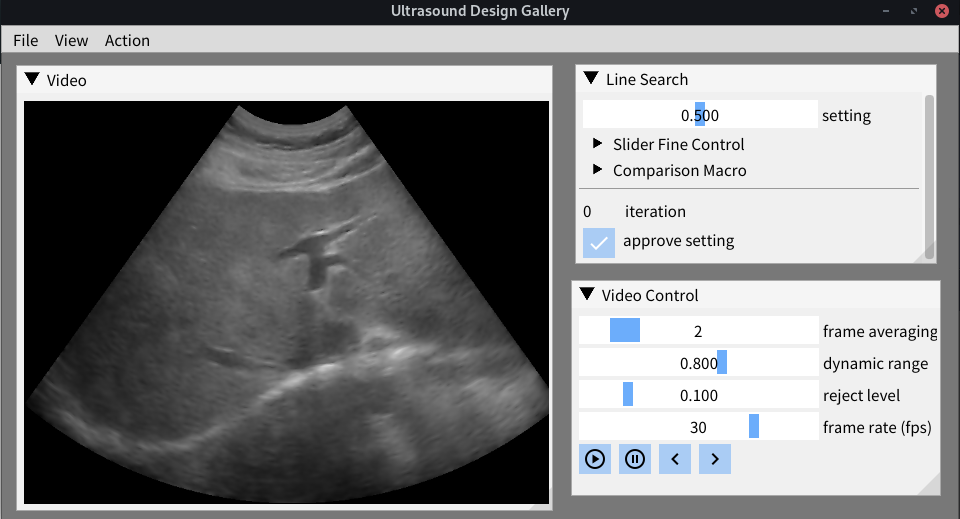
\includegraphics[scale=0.30]{figures/ui.png}
  \caption{User interface of the Ultrasound Design Gallery. We can see the \textbf{video (preview) window} (left), the \textbf{line search window} (top right), and the \textbf{video control window} (bottom right) }\label{fig:ui}
\end{figure}
%
The user interface of the Ultrasound Design Gallery is shown in~\cref{fig:ui}.
It comprises of three basic components:
    \vspace{0.05in}
\begin{enumerate}
  \item[\ding{228}] \textbf{Video (preview) window}: This window displays the image processed using the currently chosen image processing parameter setting.
    \vspace{0.05in}
  \item[\ding{228}] \textbf{Line search window}: This window contains the slider which is the 1D space where the image processing parameters are embedded.
    \vspace{0.05in}
  \item[\ding{228}] \textbf{Video control window}: This window provides basic controls of the image presentation such as dynamic range, frame rate, and the likes.
\end{enumerate}
The user is supposed to interact with the slider in~\textbf{video control window}, each slider position signifies a certain image processing parameter setting embedded on the 1D line.
The \textbf{video window} presents the image sequence processed with this setting in real time.
This process is illustrasted in~\cref{fig:interaction}
Note that the image processed and displayed through the \textbf{video window} is a pre-recorded sequence of ultrasound images.

\subsubsection{Interacting with the Ultrasound Design Gallery}
%
\begin{figure}[h]
  \centering
  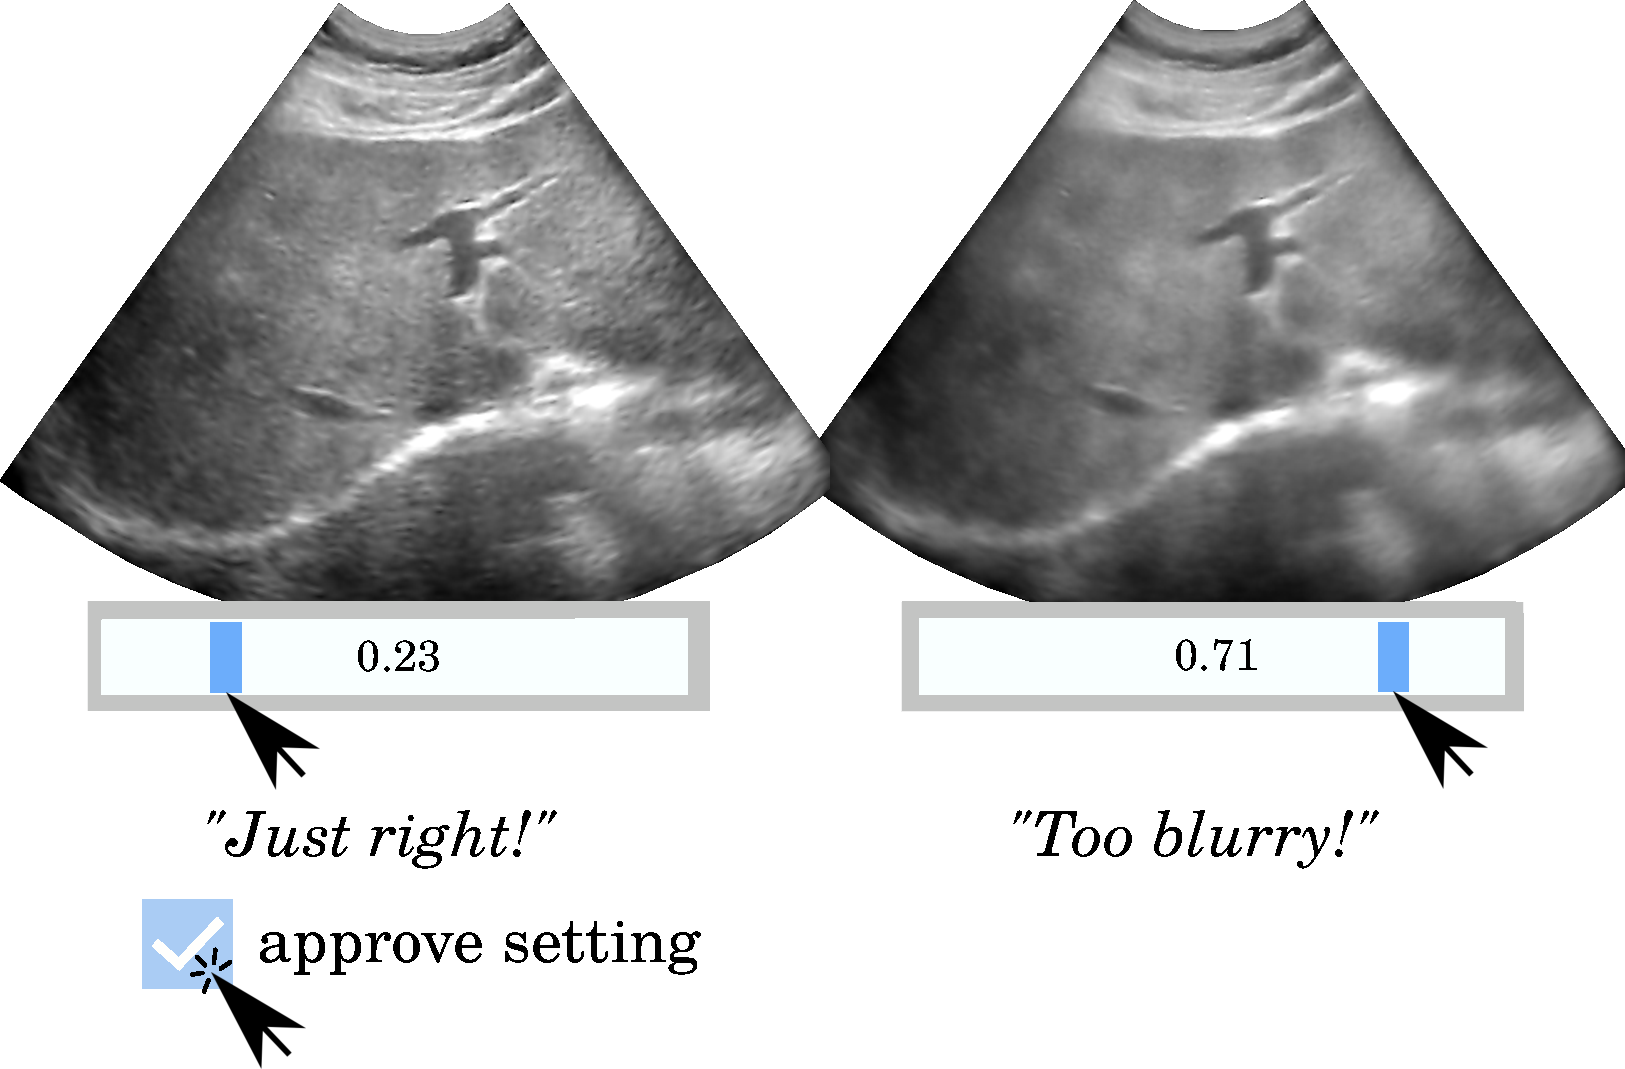
\includegraphics[scale=0.3]{figures/ui_interaction.pdf}
  \caption{Visualization of the interaction with the Ultrasound Design Gallery}\label{fig:interaction}
\end{figure}
%
The basic workflow of using the \usdg~is as follows:
\begin{enumerate}
\item[\ding{182}] The user is first presented with images processed using randomly sampled parameter settings.
\item[\ding{183}] The user compares the random settings embedded on the 1D line by interacting with the slider in the line search and approves the most preferred setting. This process is illustrated in~\cref{fig:interaction}.
\item[\ding{184}] The \usdg~records the choice and infers the visual preference function \(f\) of the user (\textbf{\cref{section:gp}}).
\item[\ding{185}] Based on the inferred probabilistic model, it recommends a new set of parameter settings using Bayesian optimization, which is also embedded on a 1D line (\textbf{\cref{section:bo}}).
\item[\ding{186}] The user compares the recommeded settings by interacting with the slider as in step~\ding{183}.
\item[\ding{187}] Go back to step~\ding{184} until convergence.
\end{enumerate}

\begin{figure}[h]
  \centering
  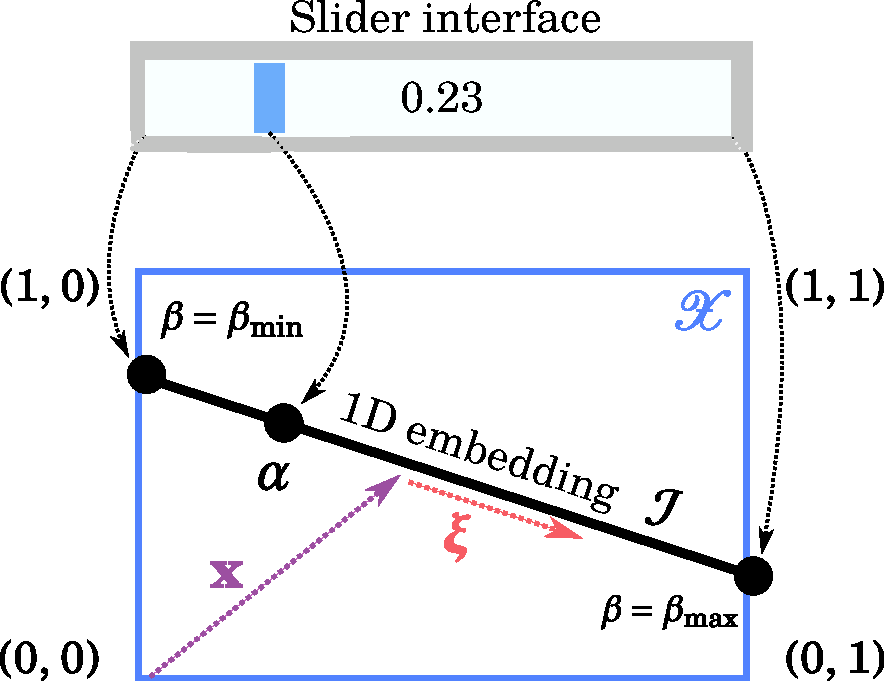
\includegraphics[scale=0.35]{figures/linesearch.pdf}
  \caption{Visualization of the relationship between the slider interface and the parameter space \(\mathcal{X}\).
    We show a two-dimensional parameter space \(\mathcal{X} = {[0, 1]}^2\) for illustration.
    The one dimensional projection is performed using the basis vector \(\vx\) and the direction vector \(\vxi\).
  }\label{fig:linesearch}
\end{figure}
%
Formally, the user solves the line seach problem
\begin{align}
 \alpha_t = &\argmax_{ \beta }\; f\,(\beta\,\vxi_t + \vx_t) \label{eq:line_search}\\
 &\text{subject to}\;\; \beta \in \mathcal{I}\left(\vx_t, \vxi_t\right) 
\end{align}
{\noindent}where \(f\) is the preference function of the user, \(\beta\) is a position on the 1D line, \(\vx_t\) and \(\vxi_t\) are respectively the basis and direction of the 1D line, \(\mathcal{X}\) is the domain of all the parameter settings, and \(\mathcal{I}\left(\vx_t, \vxi_t\right)\) is the inverval \([\beta_{\mathrm{min}}, \beta_{\mathrm{max}}]\) that ensures that \(\beta\,\vxi + \vx  \in \mathcal{X}\).
The user choice maximizing \(f\) is denoted as \(\alpha_t\).
A geometric illustration of the correspondance between the graphical interface and our mathematical notations is provided in~\cref{fig:linesearch}.

Our goal is to find the best parameter setting \(\vx^{*}\) that maximizes the user preference \(f\) given that the user successively solves this line search problem.

\subsection{Learning the Preference of Sonographers with Gaussian Processes}\label{section:gp}
\subsubsection{Probabilistic Model}
%\paragraph{Gaussian Process Formulation}
Once the user has provided his feedback, we analyze it and suggest a new 1D embedding that potentially contains the optimal parameter setting \(\vx^{*}\).
At the \(t\)th iteration, the user feedback is represented by \(\vx_t\), \(\vxi_t\) which are the sufficient information about the 1D line, and the optimal position on the line \(\alpha_t\).
Analyzing this information is posed as a machine learning problem where we reconstruct \(f\) given the history of the user choices from 1 to \(t\), \[\mathcal{D}_T = \{\,(\vx_1, \vxi_1, \alpha_1),\, \ldots\,, (\vx_t, \vxi_t, \alpha_t),\,\ldots\,, (\vx_T, \vxi_T, \alpha_T), \,\}\].

For a datapoint \( (\vx_t, \vxi_t, \alpha_t) \), each point \(\beta\,\vx_t + \vxi_t\) on the line sastisfies
\begin{align}
f(\alpha_t\,\vx_t + \vxi_t ) > f(\beta^{(i)}\,\vx_t + \vxi_t) \;\;\text{for all}\;\; \beta^{(i)} \in \mathcal{I}\left(\vx, \vxi\right) \setminus \alpha_t. \label{eq:likelihood}
\end{align}
This relationship will form our likelihood.
We will call a single instance of such comparison a ``duel'' following the preferential BO terminology~\cite{pmlr-v70-gonzalez17a}.
Each datapoint form an infinite number of duels as \(\mathcal{I}\left(\vx, \vxi\right)\) contains an infinite number of \(\beta\)s.

We perform Bayesian inference of the latent preference function \(f\) by setting a Gaussian process prior~\cite{rasmussen_gaussian_2006} on it.
Then, the overall probabilistic model is stated as 
\begin{align}
\ell          &\sim p\,(\ell) \nonumber\\
\epsilon_{\vf} &\sim p\,(\epsilon_{\vf}) \nonumber\\
\sigma        &\sim p\,(\sigma) \nonumber\\
\vf           &\sim \mathcal{GP}(0, \mK_{\ell} + \epsilon_{\vf}^2\mI) \nonumber\\
 f(\alpha_t\,\vxi + \vx_t) &> f(\beta\,\vxi_t + \vx_t),\; \forall\beta \in \mathcal{I}\left(\vx_t,\vxi_t\right) \setminus \alpha \nonumber\\
%
&\sim p\left(\alpha_t \succ \beta,\; \forall \beta \in \mathcal{I}\left(\vx_t, \vxi_t\right) \mid\, \vf,\, \sigma,\, \alpha_t,\, \vx_t,\, \vxi_t\,\right).\nonumber
\end{align}
%
    {\noindent}where \((\alpha, \vxi, \vx)\) form a single datapoint, \(\epsilon_{\vf}\) is the noise included in the preference evaluations, \(\sigma\) is the variance of the noise of the comparisons (more details in the next section), \(\vf\) is the function represented as a vector in the Gaussian process \(\mathcal{\mK}\) is the Gram matrix.

Each element of the Gram matrix is defined as
\(
  {[\mK_{\ell}]}_{i,j} = k\left(\vx^\prime_i, \vx^\prime_j; \ell \right)
\)
where \(k\left(\cdot, \cdot; \ell \right)\) is an isotropic Matern 5/2 covariance kernel with a line scale of \(\ell\), and \({\vx^\prime}_i, {\vx^\prime}_j\) are the positions formed by all the combinations of the different \(\alpha, \beta^{(i)}, \vxi, \vx\) in \(\mathcal{D}_t\).
For more details about Gaussian processes, see~\cite{rasmussen_gaussian_2006}.

\subsubsection{Likelihood}
%The most important component in our model is the likelihood function \(p\left(\alpha \, \vxi + \vx \succ \beta^{(i)} \, \vxi + \vx \mid \sigma, \vf \right)\).
Since our 1D line \(\mathcal{I}\left(\vx, \vxi\right)\) contains an \textit{infinite} number of duels between each \(\beta\) and \(\alpha\), it is difficult to formulate a proper likelihood function.
The original sequential line search design galleriy discretized the 1D line and proposed a likelihood function based on the Bradley-Terry-Luce model~\cite{10.1145/3072959.3073598}.
Since this model assumes a discrete number of comparisons, it is unclear how this discretization relates to the continuous limit.

Recently, Mikkola \textit{et al.}~\cite{pmlr-v119-mikkola20a} proposed a more principled approach that does not rely on the BTL model.
They first chose the likelihood of a single comparison to be 
\begin{align}
  &p\left(\alpha \, \vxi + \vx \succ \beta^{(i)} \, \vxi + \vx \mid \sigma, \vf \right) \\
  &= 1 - \left(\Phi * \phi \right)\left( \frac{ f\left(\beta^{(i)} \, \vxi + \vx \right) - f\left(\alpha \, \vxi + \vx \right) }{\sigma} \right)
\end{align}
{\noindent}where ``\(\succ\)'' denotes the preferential ordering between two parameter settings, \(\left(\Phi*\phi\right)\left(\cdot\right)\) is the convolution between the cummulative and probability density functions of the standard Gaussian distribution. 

At the limit of infinitely many \(\beta\)s, the likelihood of the discrete comparisons converges to the continuous ideal by the type-I Volterra integral such as
{\small
\begin{align}
  &p\left(\alpha \succ \beta,\; \forall \beta \in \mathcal{I}\left(\vx, \vxi\right) \mid\, \vf,\, \sigma,\, \alpha,\, \vx,\, \vxi\,\right) \\
  &= \lim_{N \rightarrow \infty} \prod^{N}_{i=1} p\left(\alpha \, \vxi + \vx \succ \beta^{(i)} \, \vxi + \vx \mid \sigma,\, \vf \right) \\
  &= \lim_{N \rightarrow \infty} \prod^{N}_{i=1} \left(  1 - \left(\Phi * \phi \right)\left( \frac{ f\left(\beta^{(i)} \, \vxi + \vx \right) - f\left(\alpha \, \vxi + \vx \right) }{\sigma} \right) \right) \\
  &\rightarrow \exp\left(  - \int_{\mathcal{I}\left(\vx, \vxi\right)} \left(\Phi * \phi \right) \left( \frac{ f\left(\beta \, \vxi + \vx \right) - f\left(\alpha \, \vxi + \vx \right) }{\sigma} \right) d\beta \right)
\end{align}
}%
%
{\noindent}where \(\beta^{(1)}, \ldots, \beta^{(N)}\) is taken to be an increasing sequence partitioning \(\mathcal{I\left(\vx, \vxi\right)}\).

Now, the log-likelihood of the dataset is given as
{\small
\begin{align}
  &\log p\left(\mathcal{D}_T \mid \sigma,\, \vf \right) \\
  &= \sum_{t=1}^{T} p\left(\alpha_t \succ \beta,\; \forall \beta \in \mathcal{I}\left(\vx_t, \vxi_t\right) \mid \vf,\, \sigma,\, \alpha_t,\, \vx_t,\, \vxi_t\right) \\
  &= -\sum_{t=1}^{T} \int_{\mathcal{I}\left(\vx_{t}, \vxi_{t}\right)} \left(\Phi * \phi \right) \left( \frac{ f\left(\beta \, \vxi_{t} + \vx_{t} \right) - f\left(\alpha_{t} \, \vxi_{t} + \vx_{t} \right) }{\sigma} \right) d\beta \\
  &\approx -\frac{1}{N}  \sum_{t=1}^{T} \sum_{i=1}^N \left(\Phi * \phi \right) \left( \frac{ f\left(\beta^{(i)} \, \vxi_{t} + \vx_{t} \right) - f\left(\alpha_{t} \, \vxi_{t} + \vx_{t} \right) }{\sigma} \right) d\beta
\end{align}
}%
{\noindent}where the convolution \(*\) can be accurately approximated using quadrature methods.
In our case, we use the 16-point Gauss-Hermite quadrature.
Finally, for the outer integral, Mikkola \textit{et al.} perform Monte Carlo integration by sampling \(\beta^{(1)}, \ldots, \beta^{(N)} \) from a truncated generalized normal distribution depending on \(\vx, \vxi\) and \(t\).
This choice is simply heuristic, and they adaptively concentrate \(\beta_i\) towards \(\alpha\) as \(t\) increases.
For the number of Monte Carlo samples, we set \(N=20\).

\subsubsection{Computational Costs}
Considering the likelihood approximation, the dataset is actually represented as \(\mathcal{D}_{T} = {\{\,(\,\vx_{t},\, \vxi_{t},\, \alpha_{t},\, \beta^{(1)}_{t},\, \ldots\, \beta^{(N)}_{t})\,\}}_{t=1}^{T}\).
The maximum memory requirement for storing the dataset is \(\mathcal{O}\left( T^2 \, N^2  \right)\) where evaluating the likelihood involves a Cholesky decomposition resulting in a time complexity of \(\mathcal{O}\left( T^3 \, N^3 \, M^3  \right)\) where \(T\) is the maximum number of BO iterations, \(N\) is the number of Monte Carlo samples of \(\beta\), and \(M\) is the number of quadrature points for the convolution integral.
While the computational complexity might seem unreasonable, our C++ implementation is efficient enough to maintain real-time inference on a laptop.

\begin{figure}[t]
  \removelatexerror
  \begin{algorithm2e}[H]
    \DontPrintSemicolon
    \SetAlgoLined
    \KwIn{Precomputed Cholesky decomposition of \(\mK\),
      convergence criterion, 
      gradient function of the likelihood \(\nabla_{\vf}\, p(\mathcal{D}\mid\vf)\),
      Hessian function of the joint \(\nabla^2_{\vf}\, p(\mathcal{D},\, \vf)\).
    }
    \KwOut{
      \(\vf_{t}\), \(\mW_t\).
    }
    \( \vf_1 \leftarrow \mathbf{0} \)\;
    \Repeat{ until convergence } {
      \(\valpha        \leftarrow \mK\backslash\vf_{t} \)\;
      \(\vg            \leftarrow \nabla_{\vf}\, p(\mathcal{D}\mid\vf)|_{\vf = \vf_t} - \valpha \)\;
      \(\mW_t          \leftarrow -  \nabla^2_{\vf}\, p(\mathcal{D},\, \vf) \)\;
      \(\mB           \leftarrow \mI + \mK \mW \)\;
      \(\mL_{\mB}, \mU_{\mB} \leftarrow \mathrm{lu}\,(\mB) \)\;
      \(\vp           \leftarrow \mL_{\mB} \backslash \mU_{\mB} \backslash \mK \vg \)\;
      \(\vf_{t+1}      \leftarrow \vf_t + \eta \, \vp \)\;
      \(t \leftarrow t + 1\)\;
    }
    \caption{Newton's Method for Laplace's Approximation}\label{alg:newton}
  \end{algorithm2e}
\end{figure}
%
\subsubsection{Inference with Laplace's Approximation}
We approximate the posterior \(p\,(\vf\,|\,\vtheta,\, \mathcal{D})\) with Laplace's approximation~\cite{williams_bayesian_1998}.
Laplace's approximation performs a second order Taylor expansion around the maximum of the posterior such that
\begin{align}
q\,(\vf) = \mathcal{N}\left(\vf;\, \vf^*,\, {(\mK^{-1} + \mW)}^{-1}\right) \approx p\,(\vf \mid \vtheta,\, \mathcal{D})
\end{align}
where \(\vf^*\) is the maximum a-posteriori estimate such that \(\nabla_{\vf}\, p\,(\mathcal{D},\, \vf)|_{\vf = \vf^*} = 0\), \(\mW = -\nabla^2_{\vf}\, p\,(\mathcal{D},\,\vf)|_{\vf=\vf^*} \) is the negative Hessian of the likelihood at \(\vf^*\), and \(\mK\) is the covariance matrix.
In general, \(\mH\), the Hessian of \(p\,(\mathcal{D},\vf)\) turns out structured.
This allows efficient implementations of Newton's method for finding \(\vf^*\).
For example,~\cite{rasmussen_gaussian_2006} discusses cases where \(\mH\) is diagonal or block-diagonal.
Unfortunately, in our case, the structure of \(\mH\) is neither.
We thus provide a different implementation of Newton's iteration that uses the identities
\begin{align}
  {\big(\mK^{-1} + \mW\big)}^{-1}
  &= {\Big(\mK^{-1} \big(\mI + \mK \mW \big)\Big)}^{-1} \\
  &= {{\big(\mI + \mK \mW \big)}^{-1} \mK} \\
  &= \mB^{-1} \mK \\
  &= \mU_{\mB}^{-1} \, \mL_{\mB}^{-1} \, \mK \label{eq:BinvK}
\;.
\end{align}
where \cref{eq:BinvK} is computed using the LU decomposition of \(\mB\) and back-substitution.
A detailed illustration is provided in~\cref{alg:newton} where \(\vp\) is the Newton direction, the stepsize \(\eta\) is found using backtracking line search with Armijo's condition~\cite{nocedal_numerical_2006}.

\subsubsection{Predictive Distribution}
For prediction, we use a formulation of \({\big(\mK^{-1} + \mW\big)}^{-1}\) different from~\cref{eq:BinvK}.
This is because the variance prediction \(\sigma^2(\vx)\) which requires to compute a inverse quadratic term \(\mK^{\top}(\vx) {\big(\mK^{-1} + \mW\big)}^{-1} \vk(\vx)\), which can be efficiently computed when a Cholesky decomposition of \(\mL_{\mathcal{L}} \, \mL^{-1}_{\mathcal{L}}  = {\big(\mK^{-1} + \mW\big)}\) is available.
The formulation of~\cref{eq:BinvK} does not directly provide a closed form expression for the Cholesky.
We thus use the indentities
\begin{align}
  {\big(\mK^{-1} + \mW\big)}^{-1}
  &= { \Big({\big(\mL\,\mL^{\top}\big)}^{-1} + \mW \Big) }^{-1} \label{eq:Kcholid}  \\
  &= { \big(\mL^{-\top}\,\mL^{-1} + \mW \big) }^{-1}  \\
  &= { \Big( \mL^{-\top}\,\big(\mI + \mL^{\top}\,\mW\,\mL \big)\,\mL^{-1} \Big) }^{-1}  \\
  &= \mL\,{\big(\mI + \mL^{\top}\,\mW\,\mL \big)}^{-1}\,\mL^{\top}  \\
  &= \mL\, \mC^{-1} \,\mL^{\top}  \\
  &= \big( \mL\, \mL_{\mC}^{-1} \big)\, {\big( \mL\, \mL_{\mC}^{-1} \big)}^{\top} \label{eq:Ccholid} \\
  &= \mL_{\mathcal{L}} \, { \mL_{\mathcal{L}} }^{\top}
\end{align}
where~\cref{eq:Kcholid} uses the precomputed Cholesky decomposition of \(\mK\) and~\cref{eq:Ccholid} requires the Cholesky decomposition of \(\mC = \mI + \mL^{\top}\,\mW\,\mL\).

The GP prediction using \(q\,(\vf)\) are computed as
\begin{align}
  \mu\,(\vx)
  &= {\vk(\vx)}^{\top} \mK^{-1} \, \vf^*  \\
  \sigma^2\,(\vx)
  &= k(\vx, \vx) - \vk^{\top}(\vx) \, {(\mK^{-1} + \mW)}^{-1} \, \vk(\vx) \\
  &= k(\vx, \vx) - {\big( \mL_{\mathcal{L}} \vk(\vx) \big)}^2
\end{align}

\subsubsection{Hyperparameter Treatment}
Our model has 3 hyperparameters: the covariance scale \(\ell\), the likelihood noise scale \(\sigma\), and the GP noise scale \(\sigma_\epsilon\).
We set log-normal hyperpriors such that \(\log \ell \sim \mathcal{N}\left(\text{-}1, 1\right)\), \(\log \sigma \sim \mathcal{N}\left(0, 1\right)\), and \(\log \sigma_{\epsilon} \sim \mathcal{N}\left(0, 1\right)\).
Inference is performed with type-II maximum a-posteriori (MAP-II) with the Nelder-Mead simplex method~\cite{nelder_simplex_1965}.
Although MAP-II for GP hyperparameters is often done with gradient descent, it significantly complicates the handling of Cholesky failures.

While previous works observed that the full Bayesian approach improves performance~\cite{henrandez-lobato_predictive_2014, snoek_practical_2012}, recent experimental results suggest that such performance improvement may not be significant~\cite{ath_bayesian_2021}.
In our case, the exact marginal likelihood is not available.
Thus, full Bayesian inference requires pseudo-marginal MCMC~\cite{filippone_pseudomarginal_2014, pmlr-v51-murray16} methods, which suffer in high-dimensions.
Also, the real-time nature of our application makes the use of pseudo-marignal MCMC very delicate in terms of computational efficiency and robustness.
Nonetheless, we experimented with full Bayesian inference using pseudo-marginal slice-sampling~\cite{pmlr-v51-murray16} and concluded that it is not worth the computational cost.

%Some theoretical~\cite{berkenkamp_noregret_2019} and practical~\cite{wang_adaptive_2013} works have suggested that expert tuned hyperparameters achieve better performance than full Bayesian treatments.

%% \paragraph{Pseudo-Marginal MCMC}
%% Using our approximation \(q\,(\vf)\), we use  for sampling both \(\vf\) and \(\vtheta\) from the posterior.
%% The marignal likelihood is approximated using importance sampling such that
%% \begin{align}
%%   \tilde{p}\,(\mathcal{D}\mid\theta)
%%   &= \int p\,(\mathcal{D}\mid\vf)\,p\,(\vf\mid\vtheta) d\vf \\
%%   &\approx \frac{1}{N_{\mathrm{pm}}} \sum^{N_{\mathrm{pm}}}_{i=1} \frac{p\,(\mathcal{D}\mid\vf_i)\,p\,(\vf_i\mid\vtheta)}{q\,(\vf_i)}
%% \end{align}
%% where \(\vf_i\) are samples from \(q\,(\vf)\) and \(N_{\mathrm{pm}}\) is the number of samples.
%% For simplicity, we use the maximum a-posteriori estimate \(\vf^*\).

%% For sampling \(\theta\) and \(\sigma\), we use elliptical slice sampling~\cite{murray_elliptical_2010}.
%% To resolve this problem, Murray \& Graham propose pseudo-marginal slice sampling~\cite{}.

%% Using the ARD hyperparameters alone for sensitivity analysis results is not very effective~\cite{pmlr-v89-paananen19a}.
%% Also, the non-identifiability of ARD hyperparameters complicates their statistical analysis~\cite{zhang_inconsistent_2004a}.
%% ARD is severely affected by dimensionality.
%% This manifests as low acceptance rates in MCMC procedures~\cite{filippone_pseudomarginal_2014}.

\subsection{Optimizing Preference with Bayesian Optimization}\label{section:bo}
Now that we have inferred the preference function \(f\) of the sonographer, we use Bayesian Optimization (BO) to find its optimum.
The key step of BO is the \textit{inner optimization problem} where the next 1D line formed by \(\vx_{t+1}, \vxi_{t+1}\) is determined.
Given the 1D line the user will solve the line search problem in~\cref{eq:line_search}.
The inner optimization problem is described as
%
\begin{align}
 &\maximize_{\vx,\, \vxi}\;\; a\,(\vx, \vxi \mid \mathcal{D}_t) \\
 &\text{subject to}\;\; \vx \in \mathcal{X},\; \norm{\vxi}_{\infty} = 1.
\end{align}
where \(a\,(\vx, \vxi \mid \mathcal{D}_t)\) is known as the acquisition function.
Given a GP trained on \(\mathcal{D}_t\), the acquisition function quantifies the utility of choosing \(\vx, \vxi\) next.
Naturally, choosing the right acquisition function is crucial to the convergence of BO.

\subsubsection{Approximate Expected Improvement}
Mikkola \textit{et al.}~\cite{10.1145/3072959.3073598} proposed to reformulate the popular expected improvement (EI,~\cite{jones_efficient_1998}) acquisition as
\begin{align}
  a\,(\vx, \vxi)
  = \mathbb{E}\,\Big[\, \max\big(\, \max\,\big\{\; f\,(\,\beta \xi + \vx\,) \mid \beta \in \mathcal{I} \;\big\}, 0 \,\big)\,\Big],
\end{align}
which they approximated using discrete thompson sampling (DTS) such as
\begin{align}
  &a_{\mathrm{AEI}}\,(\vx, \vxi) 
  = \frac{1}{N_{\mathrm{mc}}} \sum_{j=1}^{N_{\mathrm{mc}}} \max\,(\, \max\,\big\{\; y_i, \ldots, y_{N_\beta} \;\big\}, 0 \,) \label{eq:aei} \\
  &\text{where} \;\;  \beta_i \sim p\,(\beta), \nonumber\\
  &\quad\qquad y_i \sim \mathcal{N}\big( \mu\,(\,\beta_i \vxi + \vx \,),\, \sigma^2\,(\, \beta_i \vxi + \vx \,) \big).\nonumber
\end{align}
The outer expectation is approximated using a Monte Carlo average and \(y_i\) are the DTS samples generated from the GP predictive distribution.

Since computing gradients of~\cref{eq:aei} (whether stochastic or not) is tricky, the original implementation of~\cite{pmlr-v119-mikkola20a} uses the finite-difference approximation.
To reduce variance, they averaged a large number of stochastic gradient samples, which is less effective with higher dimensions, and significantly impacts the computational performance.
Therefore, we use an alternative acquisition function.

\subsubsection{Expected Improvement with Koyama's Scheme}
In~\cite{10.1145/3072959.3073598}, Koyama \textit{et al.} proposed a similar slider based preferential BO interface.
Here, they proposed a heuristic acquisition strategy where the slider \(\mathcal{I}\) is determined using
\begin{align}
  \vx_{\mathrm{EI}}   &= \argmax_{\vx} a_{\mathrm{EI}}(\vx) \label{eq:koyama_ei} \\
  \vx^*   &= \argmax_{\vx} \mu\,(\vx) \label{eq:koyama_opt}
\end{align}
such that \(\mathcal{I}\) interpolates \(\vx_{\mathrm{EI}}\) and \(\vx^*\).
In our case, we choose the 1D line \(\mathcal{I}\) formed by \((\vx_{t+1}, \vxi_{t+1})\) to extend across the whole space \(\mathcal{X}\).
We adapt Koyama's scheme to our setup by finding the 1D line that contains both \(\vx_{\mathrm{EI}}\) and \(\vx^*\) such that
\begin{align}
  \vx_{t+1}   = \vx_{\mathrm{EI}}\;\; \text{and} \;\;
  \vxi_{t+1} = \frac{\vx_{\mathrm{EI}} - \vx^*}{\norm{ \vx_{\mathrm{EI}} - \vx^* }_{\infty}}.\label{eq:xi_proj}
\end{align}

Koyama's scheme is neat in that both~\cref{eq:koyama_ei} and~\cref{eq:koyama_opt} have closed form deterministic gradients, enabling the use of the popular L-BFGS~\cite{liu_limited_1989} optimizer.
Also, the 1D slider chosen by the Koyama scheme contains the duel \(\vx^*\) v.s. \(\vx_{\mathrm{EI}}\), which naturally draws connections with preferential BO methods with binary discrete comparisons~\cite{NIPS2007_b6a1085a}.


\section{Cascaded Laplacian Pyramid Diffusion}\label{section:filter}

We will now discuss the image enhancement algorithm used for evaluating the Ultrasound Design Gallery.
Instead of using a previously proposed approach, we contribute our own ultrasound image enhancement algorithm, which is primarily based on Laplacian pyramids~\cite{zhang_multiscale_2006, zhang_nonlinear_2007, kang_new_2016} and anisotropic diffusion~\cite{perona_scalespace_1990, weickert_anisotropic_1998}.

\subsection{Background}
We first briefly discuss Laplacian pyramids and anisotropic diffusion before describing our cascaded Laplacian pyramid diffusion.

\subsubsection{Anisotropic Diffusion}\label{section:diffusion}
%
Diffusion partial differential equations (PDE) are popular for enhancing the quality of medical ultrasound images~\cite{perona_scalespace_1990, weickert_anisotropic_1998, contrerasortiz_ultrasound_2012}.
Especially, anisotropic diffusions have shown to reduce speckle noise~\cite{yongjianyu_speckle_2002}, strenghten image edges~\cite{zhang_multiscale_2006}, and enhance image structures~\cite{abd-elmoniem_realtime_2002, kang_new_2016} with low computational cost (see~\cite{finn_echocardiographic_2011} for a comparative evaluation of some classic anisotropic diffusions).
However, anisotropic diffusion methods are also known to be highly sensitive to their parameters~\cite{duarte-salazar_speckle_2020}, making them a perfect candidates for this study.

A generic form of anisotropic diffusion is
\begin{align}
  \frac{\partial I\,(x, y, t)}{\partial t} = \nabla \cdot [ \mD\,(x, y, t) \, \nabla I\,(x, y, t) ] \label{eq:generic_diffusion}
\end{align}
where \(I\,(x, y, t)\) is the image intensity at position \((x, y)\) and time point \(t\), \(\nabla I\) is the image gradient, and \(\mD\) is the \textit{diffusion matrix}.
Solving~\cref{eq:generic_diffusion} for a certain time period \([0, T]\) results in the enhanced image.
Different choices for determining the diffusion matrix result in completely different algorithms.

%% The diffusion matrix is most often position and time dependent but we omit the dependence on \(x, y, t\).
%% Different choices for determining the diffusion matrix result in completely different algorithms.
%% In general, the diffusion matrix is decomposed in diagonal form such as
%% \begin{align}
%%   \mD = 
%%   \left(
%%   \begin{array}{cc}
%%     \vv_1 \\
%%     \midrule
%%     \vv_2
%%   \end{array}
%%   \right)
%%   \begin{pmatrix}
%%     \lambda_1 & 0 \\
%%     0 & \lambda_2
%%   \end{pmatrix}
%%   \left(
%%   \begin{array}{c|c}
%%        \vv_1 & \vv_2
%%   \end{array}
%%   \right)
%% \end{align}
%% with respect to the eigenvectors \(\vv_1, \vv_2\) and eigenvalues \(\lambda_1, \lambda_2\).
%% The eigenvalues and eigenvectors determine how much diffusion occurs towards which direction.
%Since \(\mD\) determines how much diffusion occurs towards which direction, different diffusion matrices result in completely different behavior.

\subsubsection{Laplacian Pyramids}\label{section:pyramid}
%
Compared to other image modalities, medical ultrasound images suffer from noise artifacts, and damaged image structures.
These types of problems are difficult to detect in low pixel scales.
Therefore, multiscale approaches based on the Wavelet~\cite{xulizong_speckle_1998, xiaohuihao_novel_1999, pizurica_versatile_2003, yongyue_nonlinear_2006} and Laplacian pyramid~\cite{sattar_image_1997, zhang_multiscale_2006, zhang_nonlinear_2007, kang_new_2016} decompositions have shown great success in ultrasound images.

An \(L\)-level Laplacian pyramid~\cite{burt_laplacian_1983} is first defined using a Gaussian pyramid \(\{\vg_0,\, \ldots\, \vg_L \}\) where each level \(\vg_{i}\) is defined as
%
\begin{equation}
\begin{tikzpicture}[baseline=(current  bounding  box.center)]
	% Place nodes using a matrix
  \node[dspnodeopen, dsp/label=left]                (c0) {\(\vg_{i-1}\)};
  \node[dspsquare,   right= of c0]                  (c1) {\(G_{\sigma}\)};
  \node[dspsquare,   right= of c1]                  (c2) {\(\downarrow 2\)};
  \node[dspnodeopen, right= of c2, dsp/label=right] (c3) {\(\vg_{i}\)};
%
  \foreach \i [evaluate = \i as \j using int(\i+1)] in {0,1,2}
  \draw[dspconn] (c\i) -- (c\j);
\end{tikzpicture}
\end{equation}
%
where \(\vg_0\) is the original image, \(G_{\sigma}\) is a Gaussian low-pass filter with standard deviation \(\sigma\).
From this, the Laplacian pyramid \(\{{\boldsymbol\ell}_0,\, \ldots\, {\boldsymbol\ell}_L \}\) is defined such that each level \({\boldsymbol\ell}_i\) is defined as
%
\begin{equation}
\begin{tikzpicture}[baseline=(current  bounding  box.center)]
  \matrix (m1) [row sep=2.5mm, column sep=5mm]
  {
    \node[dspnodeopen, dsp/label=left] (g0) {\(\vg_{i+1}\)};   &
    \node[dspsquare]                   (g1) {\(2 \uparrow\)}; &
    \node[coordinate]                  (g2) {}; \\
%
    \node[dspnodeopen, dsp/label=left]  (g3) {\(\vg_{i}\)}; &
    \node[coordinate]                   (g4) {};           &
    \node[dspadder, label=94:\(-\)]     (g5) {};           &
    \node[coordinate]                   (g6) {};           &
    \node[dspnodeopen, dsp/label=right] (g7) {\({\boldsymbol\ell}_{i}\)}; \\
  };
%
  \draw[dspconn] (g0) -- (g1);
  \draw[dspline] (g1) -- (g2);
  \draw[dspconn] (g2) -- (g5);
%
  \draw[dspline] (g3) -- (g4);
  \draw[dspconn] (g4) -- (g5);
  \draw[dspline] (g5) -- (g6);
  \draw[dspconn] (g6) -- (g7);
%
\end{tikzpicture}
\end{equation}
%
where the last level is defined as \({\boldsymbol\ell}_{L} = \vg_{L}\).
Each level of the Laplacian pyramid contains an overlapping band-bass representation of the image, which can be used to detect different features in the scale space.
Higher levels (close to \({\boldsymbol\ell_{L}}\)) contain lower frequency components such as image structures while the lower levels (close to \({\boldsymbol\ell_{0}}\)) contain higher frequency components such as edges.
The original image \(I\) can be reconstructed by reducing all the levels such that \(I = \sum_{i=0}^L {\boldsymbol\ell}_{i} \).
An illustration of a 4-level conventional Laplacian pyramid based filter is shown in~\cref{fig:lpnd}.

\begin{figure*}
  \centering
  \begin{minipage}[c]{0.43\textwidth}
    \centering
    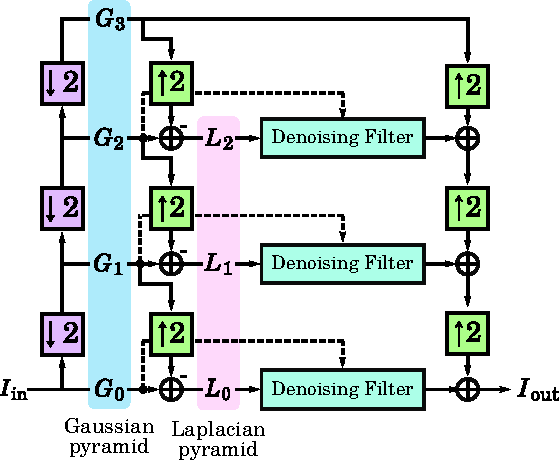
\includegraphics[scale=0.75]{figures/conventional_laplacian_pyramid.pdf}
    \subcaption{Laplacian Pyramid in Parallel Form \\ (conventional)}\label{fig:lpnd}
  \end{minipage}
  \begin{minipage}[c]{0.53\textwidth}
    \centering
    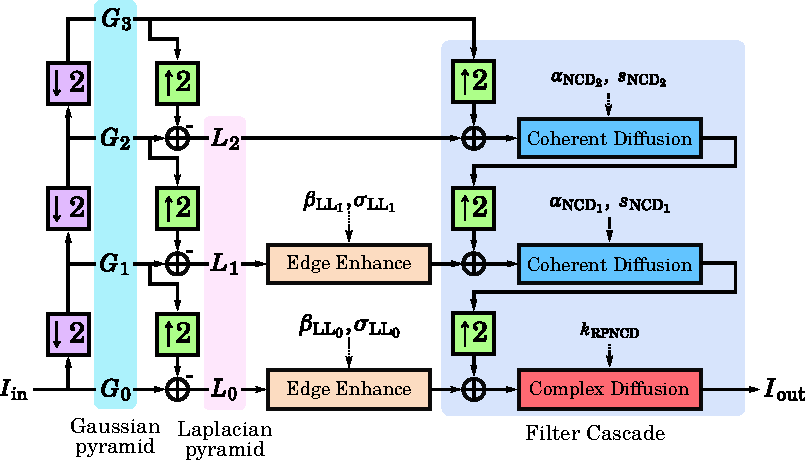
\includegraphics[scale=0.75]{figures/multiscale_filter.pdf}
    \subcaption{Laplacian Pyramid in Cascaded Form \\ (proposed)}\label{fig:clpd}
  \end{minipage}
  \caption{Block diagrams of Laplacian pyramids in parallel and cascaded form.
    Coherent diffusion denotes the NCD while complex diffusion denotes the RPNCD.
  }\label{fig:filters}
\end{figure*}
%
\subsection{Limitations of Conventional Laplacian Pyramids}\label{section:limitations}
\subsubsection{Conventional Laplacian Pyramids Filters}
As illustrated in~\cref{section:pyramid}, Laplacian pyramids are based on a band-pass decomposition of the image.
Previous Laplacian pyramid approaches modified the intermediate Laplacian image \({\boldsymbol\ell_i}\) so that the reconstructed image is enhanced.
For example, Zhang \textit{et al.} applied anisotropic diffusion~\cite{perona_scalespace_1990} and shock filters~\cite{zhang_multiscale_2006} to each Laplacian image.
More recently, Kang \textit{et al.}~\cite{kang_new_2016} applied different types of anisotropic diffusion filters to each level so that their corresponding features are enhanced appropriately.
However, these previous approaches have been ignoring some issues that should be raised when combining conventional filters with Laplacian pyramids.

\subsubsection{Limitations of Conventional Laplacian Pyramids}
Conventional image enhancement algorithms, especially anisotropic diffusion methods, are designed to work on low-pass or full-bandwidth images.
Therefore, it is questionable whether applying these algorithms to the Laplacian band-pass images is appropriate.
For example, most anisotropic diffusion methods perform some sort of edge-detection, which is not straightforward to perform on band-pass images.
Indeed, Zhang \textit{et al.} circumvented this issue by first performing diffusion on \(\vg_{i}\)
performing edge-detection on the low-pass image \(\vg_{i}\) and then perform diffusion on \({\boldsymbol\ell}_{i}\)~\cite{zhang_multiscale_2006}.
Still, it is unknown whether diffusing on the band-pass image results in ideal behavior.

Previous Laplacian pyramid approaches only applied filters in parallel to each \({\boldsymbol\ell}_i\).
That is, no information is propagated across different levels.
This is wasteful since each level in the pyramid contain different feature information that could reinforce filtering at other levels.
Espacially, higher level Laplacian images contain structural information that are less affected by noise.

\subsection{Cascaded Filters in Laplacian Pyramids}
\subsubsection{Laplacian Pyramids in Cascaded Mode}
We will now present our new Laplacian pyramid based schema: the \textsc{Cascaded Laplacian Pyramid Filter}.
We utilize the Laplacian pyramid in \textit{cascaded form}, which does not have the limitations of the conventional \textit{parallel form} discussed in~\cref{section:limitations}.
Filtering is performed top level first to bottom level last, so that lower levels can fully utilize the ifnromation acquired from the higher levels.
Also, each level of our filter form a low-pass image, which is fully compatible with conventional anisotropic diffusion filters.

First, at the top level, recall that \({\boldsymbol\ell}_L = \vg_L\).
By applying an arbitrary image enhancement filter \(F_L\left(\cdot\right)\), we obtain the filtered result \( \widehat{\vg}_L = F_L \left( \vg_L \right) \).
Now, at each level, filtering is performed as
%
\begin{equation}
\begin{tikzpicture}[baseline=(current  bounding  box.center)]
  \matrix (m1) [row sep=2.5mm, column sep=5mm]
  {
    \node[dspnodeopen, dsp/label=left] (g0) {\(\widehat{\vg}_{i+1}\)};   &
    \node[dspsquare]                   (g1) {\(2 \uparrow\)}; &
    \node[coordinate]                  (g2) {}; \\
%
    \node[dspnodeopen, dsp/label=left]  (g3) {\({\boldsymbol\ell}_{i}\)}; &
    \node[coordinate]                   (g4) {};        &
    \node[dspadder]                     (g5) {};        &
    \node[dspsquare]                    (g6) {\(F_i\)}; &
    \node[dspnodeopen, dsp/label=right] (g7) {\(\widehat{\vg}_{i}\)}; \\
  };
%
  \draw[dspconn] (g0) -- (g1);
  \draw[dspline] (g1) -- (g2);
  \draw[dspconn] (g2) -- (g5);
%
  \draw[dspline] (g3) -- (g4);
  \draw[dspconn] (g4) -- (g5);
  \draw[dspline] (g5) -- (g6);
  \draw[dspconn] (g6) -- (g7);
%
\end{tikzpicture}
\end{equation}
%
where \(\widehat{\vg}_{0}\) is the reconstructed enhanced image and the summation of \(\widehat{\vg}_{i+1}\) and \({\boldsymbol\ell}_{i}\) results in a low-pass image, which is passed to \(F_i\).
\begin{enumerate}
  \item[\ding{232}] \(\widehat{\vg}_{i+1}\) contains the full low frequency information and the enhanced features.
  \item[\ding{232}] \({\boldsymbol\ell}_{i}\) contains both noise and high frequency features (higher compared to that of \(\widehat{\vg}_{i+1}\))
\end{enumerate}
From the sum of \(\widehat{\vg}_{i+1}\) and \({\boldsymbol\ell}_i\), \(F_i\) is now able to utilize information from the upper levels when suppressing the noise and ehancing the features.
Notice that the enhancement filters \(F_0,\, \ldots\, F_L\) are \textit{cascaded} over and over to the propagated signal \(\widehat{\vg}_{i}\), hence cascaded form.
A full illustration of a 4-level cascaded Laplacian pyramid is shown in~\cref{fig:clpd}.
Notice the difference with~\cref{fig:lpnd}. 

\subsubsection{Edge-Enhancement with Laplacian Pyramids}
%
While anisotropic diffusion alone is known to have edge-enhancing effects~\cite{weickert_anisotropic_1998}, employing additional edge-enhancement filters often improve the perceived quality of medical images.
However, apart from shock filters~\cite{zhang_multiscale_2006, kang_new_2016}, edge-enhancement have been overlooked in the context of medical ultrasound images.
Conventionly, Laplacian pyramids provide a convenient way to boost edges and contrast~\cite{vuylsteke_multiscale_1994, stahl_noiseresistant_1999, dippel_multiscale_2002}.

The image Laplacian operator is often used as an edge detector.
Obtaining the Laplacian image \({\boldsymbol\ell_i}\) is equivalent to a image Laplacian operation.
Therefore, the Laplacian pyramid already provides a multi-scale representation of the edges.
Indeed the MUSICA algorithm~\cite{vuylsteke_multiscale_1994} have shown great success in radiographies and mammographies by simply amplify the Laplacian images.
However, it tend to be sensitive to noise, as it amplifies small contrasts according to a power law.
While Stahl \textit{et al.} relaxed this by linearly amplfying contrasts below a threshold~\cite{stahl_noiseresistant_1999}, this is still insufficient for ultrasound images.
Therefore, we use an amplfyer function \(g\left(\cdot\right)\) inspired by~\cite{10.1145/2010324.1964963} that strongly penalizes weak contrast such as
\begin{align}
  g\left(x; \sigma, \beta \right) =
  \begin{cases}
    \;\mathrm{sign}\left( x \right) \, \sigma \, {\left( |x|/\sigma \right)}^2, & \text{if}\; |x| \leq \sigma \\
    \;\mathrm{sign}\left( x \right) \left( \beta \left(|x| - \sigma \right) + \sigma \right), & \text{otherwise}
  \end{cases}
\end{align}
where \(\sigma\) is the threshold for small contrast.
%
\begin{figure}[H]
  \centering
  \begin{tikzpicture}[
      declare function={
        func(\x) = and(\x <= 0.3, \x >= 0) * (0.3*(abs(\x) / 0.3)^(2)) + 
        and(\x >= -0.3, \x < 0) * (-1*0.3*(abs(\x) / 0.3)^2) +
        (\x > 0.3)  * (4*(abs(\x) - 0.3) + 0.3) +
        (\x < -0.3) * ((-1)*(4*(abs(\x) - 0.3) + 0.3));
     } 
    ]
    \begin{axis} [
        axis lines=center,
        ylabel=\(g\left(x\right)\),
        xlabel=\(x\),
        width=6cm,
        height=4cm
      ]
      \addplot [domain=-1:1, smooth, thick, blue] { func(x) };
    \end{axis}
  \end{tikzpicture}
  \caption{Plot of the amplifier function \(g\) with \(\sigma=0.3\), \(\beta=4\).}\label{fig:amp}
\end{figure}
%
An exmaple plot is shown in~\cref{fig:amp}.
We can see that the low contrast values close to \(x=0\) are suppressed and large contrast values are linearly amplified by \(\beta=4\).

In the context of the cascaded Laplacian pyramid, we amplify the Laplacian image \({\boldsymbol\ell}_i\) using \(\vg_i\) before adding \(\widehat{\vg}_i\).
Therefore, both the edges and noise are amplified when entering the enhancement filter \(F_i\), and the appropriate factor \(\beta\) will thus depend on the characteristics of \(F_i\).

\subsubsection{Cascading Anisotropic Diffusion Filters}
For the filters \(F_0,\,\ldots\,, F_L\) in the cascaded Laplacian diffusion, we follow the approach of~\cite{kang_new_2016} and use a different filter for each level.
In particular, we leverage the nonlinear coherent diffusion (NCD,~\cite{abd-elmoniem_realtime_2002}) and ramp-preserving nonlinear complex diffusion (RPNCD,~\cite{gilboa_image_2004}) filters.
Both NCD and RPNCD can be efficiently implemented on GPUs and show good performance for our purpose.
Recently introduced diffusion filters based on probabilistic tissue segmentation~\cite{hutchison_probabilisticdriven_2010, ramos-llorden_anisotropic_2015} require accurately estimating a probabilistic mixture model during execution, which is both computationally expensive and difficult to take advantage of GPUs.
The method proposed by Mishra et al.~\cite{mishra_edge_2018} involves computing histogram of oriented gradients in the superpixel domain, which also cannot take advantage of GPUs.
%
\begin{figure}[H]
  \centering
  \subfloat[Original]{
    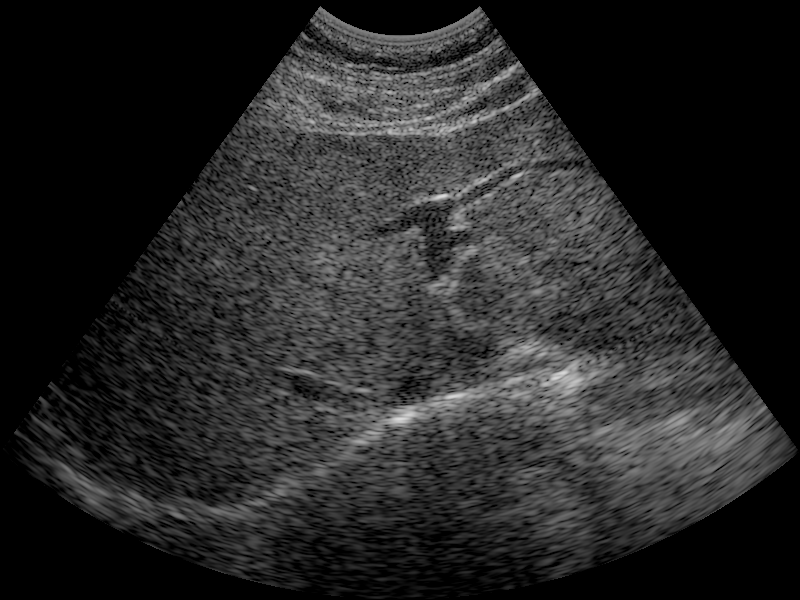
\includegraphics[trim={10cm, 10cm, 12cm, 5cm}, clip, scale=0.3]{figures/ncd_liver1.png}
  }
  \subfloat[NCD]{
    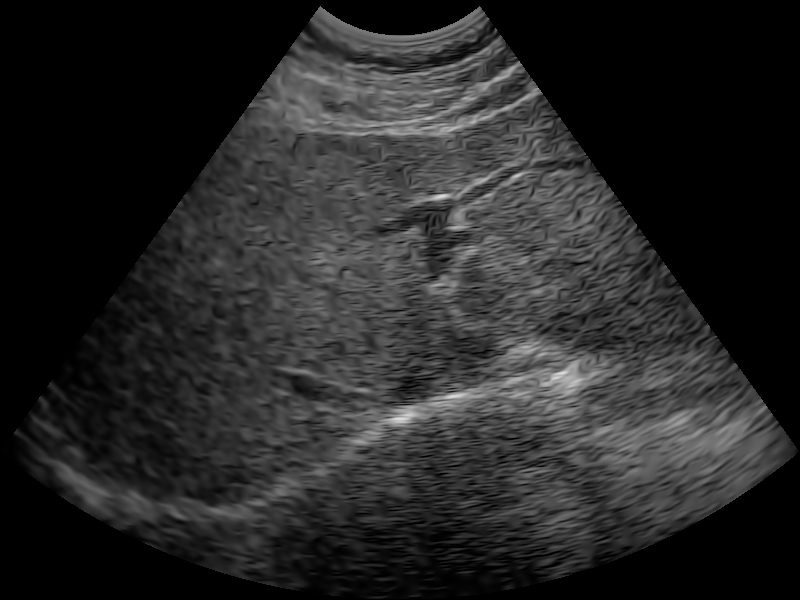
\includegraphics[trim={10cm, 10cm, 12cm, 5cm}, clip, scale=0.3]{figures/ncd_liver2.png}\label{fig:ncd}
  }
  \subfloat[RPNCD]{
    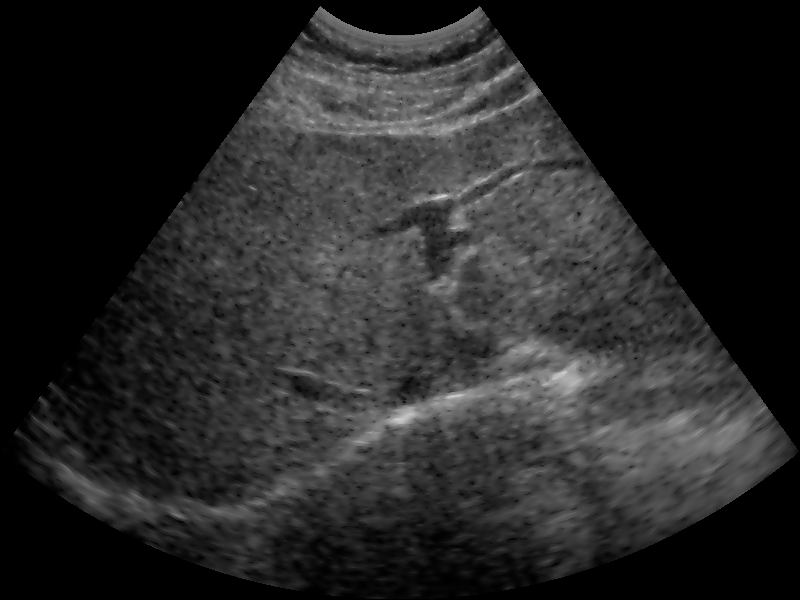
\includegraphics[trim={10cm, 10cm, 12cm, 5cm}, clip, scale=0.3]{figures/rpncd_liver.png}\label{fig:rpncd}
  }
  \caption{Liver image processed with NCD and RPNCD.}\label{fig:ncd_liver}
\end{figure}
%

Upper levels of the Laplacian pyramid contain macro structural features.
In these levels, it is important to enhance large structures such as the myocardium in echocardiographic images, or the portal veins in the liver.
Also, since upper levels contain the low frequency bands, they contain less noise, which allows aggressive filtering.
For this purpose we leverage NCD, which enhances spatial coherence.
When naively applied to ultrasound images, coherence enhancement tends to interact badly with speckle noise, resulting in artistic flow-like artifacts as shown in~\cref{fig:ncd}.
Therefore, at last, NCD will be able to display its true potential when used in the upper levels of the cascaded Laplacian pyramid.

On the other hand, lower levels contain lots of speckle noise, and less structural information.
Therefore, on the lower levels, a filter with good speckle reduction property and good edge preservation shall be used.
Ironically, most anisotropic diffusion filters perform some sort of edge-detection, which leaves us with a chicken-and-egg problem.
On the other hand, anisotropic diffusion filters based on Kuan and Lee's coefficients~\cite{yongjianyu_speckle_2002, aja-fernandez_estimation_2006, krissian_oriented_2007} tend to result in blurry images that are less desirable.
Instead, we propose to use RPNCD, which is based on a complex formulation of the anisotropic diffusion equation.
Gilboa \textit{et al.} showed that the phase evolution of the complex diffusion acts as a smoothed Laplacian edge-detector, which is highly robust to noise.
Although the RPNCD has not been used for ultrasound images, we found that it shows excellent speckle reduction properties, as shown in~\cref{fig:rpncd}.

The overall cascaded Laplacian pyramid with edge-enhancement and our filters of choice is shown in~\cref{fig:clpd}.
We use the NCD for the top two levels while the RPNCD is used only in the bottom level.
Edge enhancement is only performed on the bottom two levels.
The image pixels intensities are generally in \([0, 1]\), but we rescale the input of the NCD to \([0, 255]\) and 
For the NCD, we 

\subsubsection{Parameters of the Cascaded Laplacian Pyramid}
Our specific instance of the cascaded Laplacian pyramid has 4 levels (3 decimations).
For the pre-aliasing filter before decimation, we use a Gaussian low-pass filter with standard deviation 1.
We use a decimation rate of 2 for all levels.
The two edge-enhancement steps have two parameters each: the contrast threshold \(\sigma_{\mathrm{LL}}\) and the gain \(\beta_{\mathrm{LL}}\).
Each of the NCDs originally have 6 parameters: the smoothing rate of the structure tensor \(\rho\), the step size \(\Delta t\), the number of iterations \(N_{\text{iter.}}\), the diffusion threshold \(s\), the diffusion strength coefficient \(\alpha\).
We set \(\rho = 2\), \(\Delta t = 2\), and \(N_{\text{iter.}} = 10\).
The other parameters are tuned by the~\usdg.
The RPNCD has 4 parameters: the edge threshold \(k\), the phase angle \(\theta\), the step size \(\Delta t\), and the number of iterations \(N_{\text{iter.}}\).
We set \(\theta = 5^{\circ}\) as proposed in~\cite{gilboa_image_2004}, \(\Delta t = 0.3\), and \(N_{\text{iter.}} = 20\).
The edge threshold \(k\) is tuned by the~\usdg.

While ideally we would tune all the parameters using the~\usdg, BO takes longer to converge in high-dimensions.
Therefore, we reduced the number of parameters as possible.
Also, nonlinearity between parameters make the optimization problem fundamentally more challenging.
This happens when different parameters strongly depend on each other, or have a similar effect.
A typical example is the diffusion step size \(\Delta t\) and iteration number \(N_{\text{iter.}}\), where their effect is determined by the product (diffusion time) \(\Delta t \cdot N_{\text{iter.}}\).

\begin{table}
  \centering
  \caption{Parameters Tuned by the~\usdg}\label{table:params}
  \begin{threeparttable}
  \begin{tabular}{llrl}
    \toprule
    \multicolumn{1}{c}{\textbf{Parameter}}
    & \multicolumn{1}{c}{\textbf{Origin}}
    & \multicolumn{1}{c}{\textbf{Range}}
    & \multicolumn{1}{c}{\textbf{Scale}}
    \\ \midrule
    \(\sigma_{\mathrm{LL}_0}\), \(\sigma_{\mathrm{LL}_1}\)  & Edge-Enhance & [\(10^{\text{-}4}\), \(10^{\text{-}2}\)] & Exp.  \\
    \(\beta_{\mathrm{LL}_0}\), \(\sigma_{\mathrm{LL}_1}\)   & Edge-Enhance & [1, 5]                   & Lin. \\
    \(\alpha_{\mathrm{NCD}_1}\), \(\alpha_{\mathrm{NCD}_2}\) & NCD          & [\(0.03\), \(0.1\)]     & Lin.  \\
    \(s_{\mathrm{NCD}_1}\), \(s_{\mathrm{NCD}_2}\)           & NCD          & [\(1\), \(100\)]        & Lin. \\
    \(k_{\text{RPNCD}}\)                                & RPNCD        & [\(10^{\text{-}4}\), \(10^{\text{-}2}\)] & Exp. \\\bottomrule
  \end{tabular}
  \end{threeparttable}
\end{table}
%
The ranges and scales of the parameters to be tuned by the~\usdg~are organized in~\cref{table:params}.
A total of 9 parameters are used, resulting in a 9-dimensional optimization problem.
The number in the subscript denote the level they are used within the pyramid (also refer to~\cref{fig:clpd}).
The range \([0, 1]\) used by the~\usdg~is transformed either linearly (Lin.) or exponentially (Exp.) to the range of each parameter.

%% \begin{align}
%%   \mT = K_{\rho} * \left( \nabla_{\sigma} I \; {\nabla_{\sigma} I}^{\top} \right) 
%% \end{align}
%% where \(K_{\rho}\) is a Gaussian smoothing filter with standard deviation \(\rho\), \(\nabla_{\sigma}I\) is the gradient of \(I\) smoothed with a Gaussian filter with standard deviation \(\sigma\).
%% NCD is known to 

%% Smoothing the outer product of the gradient with \(K_{\rho}\) improves the spatial coherence of the diffusion directions.
%% For the diffusion strengths \(\lambda_1\) and \(\lambda_2\), NCD uses the eigenvalues of the structure tensor \(\mu_1\) and \(\mu_2\) such that
%% \begin{align}
%%   \lambda_1 &= \begin{cases}
%%     \; \alpha \, \left(1 - \frac{\kappa}{s^2}\right) &  \text{if}\quad \kappa < s^2  \\
%%     \; 0 & \text{otherwise}\quad
%%     \end{cases} \\
%%   \lambda_2 &= \alpha
%% \end{align}
%% where \(\kappa = {(\mu_1 - \mu_2)}^2\), \(s\) is a threshold determining the amount smoothing towards \(\vv_1\), and \(\alpha\) determines the overall amount of smoothing.
%% While the original NCD algorithm uses a regularization term \(\beta\), we ommited it as we did not find it useful.

%% Meanwhile, Gilboa et al.~\cite{gilboa_image_2004} proposed a novel diffusion scheme that circumvents the need for explicit edge detection.
%% They proposed the \textit{ramp-preserving nonlinear complex diffusion} (RPNCD) which is described as
%% \begin{align}
%%   \frac{\partial  I\,(x, y, t)}{\partial t} &= \nabla \cdot \big(\, c\,(x, y, t) \, \nabla I(x, y, t) \big) \\
%%   c\left(x, y, t\right) &= \frac{e^{j \theta}}{ 1 + {\left( \frac{\mathrm{Im}\left(I(x, y, t)\right)}{ k \, \theta } \right)}^2}
%% \end{align}
%% where \(k\) is an edge threshold, \(\mathrm{Im}\left(I(x, y, t)\right)\) is the imaginary part of \(I(x,y,t)\), \(\theta\) is a phase angle parameter.
%% Here, \(\mathrm{Im}\left(I(x, y, t)\right)\) acts as an edge detector which behaves similarly as the smoothed image laplacian.


%% While many speckle reduction algorithms have been designed to be used on a single scale, many of these algorithms can be improved by considering \textit{multiple image scales}.
%% The two most popular approaches are based on the wavelet decomposition and the Laplacian pyramid decomposition.

%% Multiscale analysis 

%% \cite{10.1145/2010324.1964963}


%% \subsubsection{Overview}


%% \paragraph{Diffusion Strength and Edge Detection}
%% While various alternative choices for determining \(\lambda_1, \lambda_2\), have been proposed over the years, most of them require some form of edge detection.
%% Therefore, accurate edge-detection must be performed \textit{before} we perform speckle reduction, which is particularly challenging.
%% In the case of NCD, \(\kappa = {(\mu_1 - \mu_2)}^2\) acts as an edge detector which provides a good cost-performance tradeoff when used as a primary edge-detector for speckle reduction.

%% While some alternatives have been introduced over the years, they either provided a poor cost-performance benefit, or turned out to be system dependent.
%% For example, Yu et al.~\cite{yu_ultrasound_2010} proposed to use the smallest univalue segment assimilating nucleus (SUSAN,~\cite{smith_susan_1997}) edge detector while Mei et al.~\cite{mei_phase_2020} proposed to use phase assymetry (PAS,~\cite{kovesi_image_1999}).
%% While SUSAN is very robust, it requires large computation windows which harms its cost-performance benefits.
%% On the other hand, the PAS detector showed excellent results on the data used by Mei et al., but performed poorly on the data that we used for this study.
%% This suggests that PAS is highly dependent on the properties of the ultrasound system it is applied.

%%% Local Variables:
%%% TeX-master: "master"
%%% End:



\begin{table*}
  %\vspace{-0.2in}
  \centering
\begin{threeparttable}
  \caption{Implementations and Parameter Settings of the Considered Baselines}\label{table:baselines}
\begin{tabular}{llclc}\toprule
  \multicolumn{1}{c}{\textbf{Algorithm}}          &
  \multicolumn{1}{c}{\textbf{Classification}}     &
  \multicolumn{1}{c}{\textbf{Implementation}}     &
  \multicolumn{1}{c}{\textbf{Parameter Settings}} &
  \multicolumn{1}{c}{\textbf{Reference}} \\\midrule
  OSRAD  & Diffusion       & Custom            & \(W_{\text{kuan}}= 5 \times 5\), \(c_{\text{tang}} = 0.1\), \(N_{\text{iteration}}=30\), \(\Delta t = 1\) & \cite{krissian_oriented_2007}  \\
  ADMSS  & Diffusion       & Official\tnote{1} & \(N_{\text{class}} = 4\), \(N_{\text{memory}}=5\), \(N_{\text{iteration}} = 20\), \(\sigma = 0.1\), \(\rho = 0.1\)  & \cite{ramos-llorden_anisotropic_2015} \\
  LPNDSF & Diffusion       & Custom            & \(r = [0.1, 1.0, 0.1]\), \(k = [0.3, 0.1, 0.1]\) & \cite{zhang_multiscale_2006} \\
  MNLM   & Non-local mean  & Custom            & \(M = 19 \times 19\), \(K = 3 \times 3\), \(I = 5\), \(h=0.1\) & \cite{breivik_realtime_2017} \\
  NLLR   & Non-local mean \& Low-rank recon.   & Official\tnote{2} & \(H = 10\), \(\beta = 10\) & \cite{zhu_nonlocal_2017} \\
  PFDTV  & Diffusion \& TV regularization    & Custom\tnote{3}   & \(N_{\text{iteration}} = 10\), \(s=15\) & \cite{mei_phase_2020} \\
  \bottomrule
\end{tabular}
\begin{tablenotes}
  \item[1] \url{https://www.mathworks.com/matlabcentral/fileexchange/52988-anisotropic-diffusion-with-memory-based-on-speckle-statistics-for-ultrasound-images}
  \item[2] \url{https://appsrv.cse.cuhk.edu.hk/~lzhu/webpage_despeckling_cvpr2017/index.html}
  \item[3] Based on the official implementation available at \url{https://github.com/Binjie-Qin/PFDTV}.
\end{tablenotes}
\end{threeparttable}
\vspace{-0.1in}
\end{table*}

%%% Local Variables:
%%% TeX-master: "master"
%%% End:

%

\section{Experiments}\label{section:eval}
\subsection{Experimental Setup}
\subsubsection{Experiment Design}
%\paragraph{Sonographer Subjects}
We recruited five sonographers and a cardiologist (also referred to as ``a sonographer'') from the Kangbuk Samsung Hospital Total Healthcare Center (Seoul, South Korea, Republic of).
All five sonographers are Registered Diagnostic Cardiac Sonographers (RDCS) certified by the American Registry for Diagnostic Medical Sonography (ARDMS) with at least three years of practicing experience.
The cardiologist has ten years of practicing clinical experience.
For convenience, the sonographers are alphabetically coded from A to F where A is the cardiologist.

\begin{table}
  \centering
  \caption{Hardware used for the Experiments}\label{table:specs}
  \begin{threeparttable}
  \begin{tabular}{ll}
    \toprule
    \multicolumn{1}{c}{\textbf{Type}}
    & \multicolumn{1}{c}{\textbf{Model and Specifications}}
    \\ \midrule
    Processor & Intel i7--7700HQ, 2.8 GHz (maximum 3.8 GHz) \\
    GPU       & Nvidia GeForce GTX 1050 Mobile \\
    Display   & Sharp LQ156D1, 15.6 inch, \(3840 \times 2160\), 282ppi  \\
    Memory    & 16GB DDR4--2400 \\ \bottomrule
  \end{tabular}
  \end{threeparttable}
\end{table}
%
%\paragraph{Experiment Protocol}
Each of the sonographers were given access to the~\usdg~through the same laptop (detailed speficiation shown in~\cref{table:specs}).
The sonographers are asked to interact with the~\usdg~until the iteration counter indicates 15.
The first 4 iterations use random settings such that \(\vx\) is a random uniform vector and \(\vxi\) is sampled from a unit \(L_{\infty}\) hypersphere.

The sonographers were instructed to freely interact with the video control panel at any time.
More importantly, they were informed to base their decisions only on the \textit{current} slider.
Without this, some sonographers were unable to make a decision becase they indiferently disliked all the positions on the slider.
Also, there were cases where all of the positions on the slider resulted in visually indistinguisable images.
In such case, we instructed the sonographers to choose a random position.

For evaluating the final results, we compute the setting maximizing the mean utility function of each sonographer such that \( \vx^* = \argmax_{\vx} \mu\left(\vx \mid \mathcal{D}_{15} \right) \).
The CLPD setting acquired from each sonographer is denoted as CLPD-A to CLPD-F where the trailing letter is the sonographer code.

\subsubsection{Ultrasound Image Data}
We use three \textit{in vivo} ultrasound image sequences.
One with a liver subcostal view, a echocardiographic 4-chamber view, and a echocardiographic parasternal long-axis view.
The liver subcostal and echocardiographic 4-chamber views were scanned at Sogang University, Seoul, South Korea from a volunteer under an IRB approvde protocol using Samsung a Accuvix V10 scanner with a Samsung C2--5EL convex probe, while the echococardiac parasternal long-axis sequence was acquired using a GE Vivid E90 scanner with a GE M5Sc-D phased probe.
The echocardiographic 4-chamber view data was extracted from the CAMUS challenge dataset~\cite{leclerc_deep_2019}, which used a GE Vivid E95 scanner with a GE M5S probe.

Since the Samsung Accuvix V10 scanner research package only returns beamformed radio-frequency (RF) data, we locally performed DC rejection, envelope detection, and scan conversion.
The RF data has 128 scanlines, which we lateral interpolate by a factor of 8.
A prealias filter was used before scan conversion.
For the GE Vivid E90 scanner, we extracted the quantized unprocessed images from the raw DICOM files, and performed scan conversion.

\subsubsection{Image Enhancement Baselines}
We evaluate the USDG-tuned CLPDs against a diverse range of speckle reduction algorithms.
Among diffusions, we compare against the oriented speckle reducing anisotropic diffusion (OSRAD,~\cite{krissian_oriented_2007}), the anisotropic diffusion filter with memory based on speckle statistics (ADMSS,~\cite{ramos-llorden_anisotropic_2015}), and the multiscale nonlinear diffusion and shock filter (LPNDSF,~\cite{zhang_multiscale_2006}).
Among non-local means based methods, we compare against the multiscale non-local means (MNLM,~\cite{breivik_realtime_2017}), and the non-local low-rank patch recovery (NLLR,~\cite{zhu_nonlocal_2017}).
Lastly, we compare against the phase asymmetry ultrasound despeckling with fractional anisotropic diffusion and total variation (PFDTV,~\cite{mei_phase_2020}).

\subsubsection{Implementations and Tuning of the Baselines}
To ensure a fair comparison, we use the official implementations whenever available.
The implementations and parameter settings of the considered baselines are organized in~\cref{table:baselines}.
For the case of OSRAD, MNLM, LPNDSF, and PFDTV, we reimplemented them according to the descriptions in the original papers.
While the official implementation of PFDTV is publically available online, we had to reimplement it due to numerical issues.

%\paragraph{Issues with Pixel Spacing}
For the NLLR and PFDTV, the pixel spacing of the data used in the original works (\(300 \times 225\)) differed significantly with ours (our images are \(800 \times 600\)).
Because of this, when applied to our data, the results were qualitatively different from those reported in the original papers.
Thus, for PFDTV and NLLR, we downscaled the images by \(40\%\), applied the respective methods, and then upscaled them back.

%\paragraph{Input Transformations}
While often not clearly stated, ultrasound image algorithms tend to use various input formats.
OSRAD requires the input to be in natural scale rather than logarithmic scale.
Therefore, for OSRAD, we decompress the log-compressed images as recommended by~\cite{yongjianyu_generalized_2004} and then recompress the output.
Other than OSRAD, use log-compressed images with pixel intensities in the range of \([0, 255]\).

\subsubsection{Metrics}
For objective quality assessment, we apply the following quality metrics to the image \textit{without} dynamic range adjustment.
All results are presented up to three significant digits.

\paragraph{(Speckle) Signal-to-Noise Ratio (SNR)}
The SNR measures the amount of speckle noise relative to the mean response of a region-of-interest.
It is given as
\begin{align}
  \mathrm{SNR} \texttt{[dB]} = 10 \log_{10} \frac{\mu}{\sigma}
\end{align}
where \(\mu\) is the mean response and \(\sigma\) is the standard deiviation of the region-of-interest.
When computed against a fully-formed speckle region, the SNR is called the \textit{speckle} SNR (SSNR).
In this case, \(\sigma\) corresponds to the noise standard deiviation.
We present the SNR in decibel scale.


\begin{figure*}
  \centering
  \begin{subfigure}[b]{0.15\textwidth}
    \begin{tikzpicture}[
        spy using outlines={%
          rectangle,magnification=3,size=\textwidth,
          every spy on node/.append style={transparentwindow}
        }
      ]
      \node (figA) at (0.0,0.0) {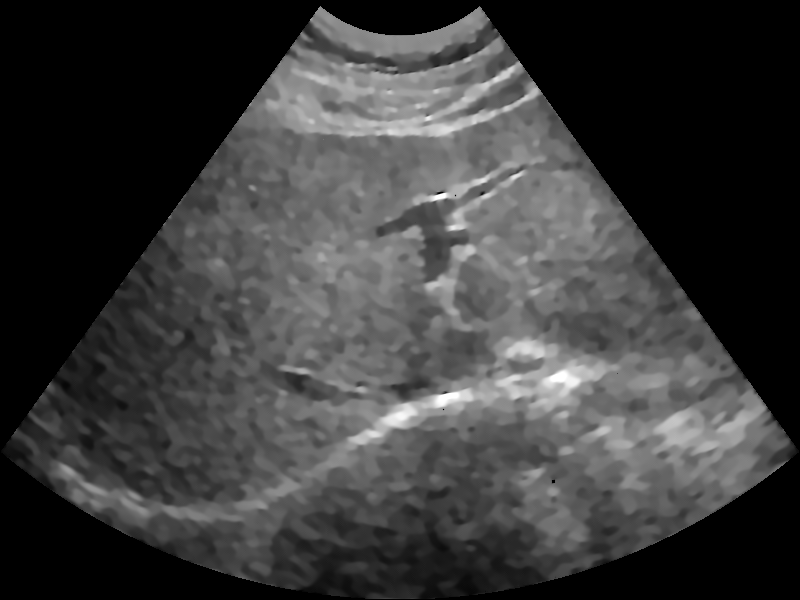
\includegraphics[width=\textwidth, trim={4cm 4cm 4cm 0cm}, clip]{figures/liver1_osrad.png}};
      \spy on (0.15, 0.0) in node [redwindow, anchor=north] at ($(figA.south)$);
    \end{tikzpicture}
    \caption{OSRAD}\label{fig:liver1_osrad}
  \end{subfigure}%
  \begin{subfigure}[b]{0.15\textwidth}
    \begin{tikzpicture}[
        spy using outlines={%
          rectangle, magnification=3,size=\textwidth,
          every spy on node/.append style={transparentwindow}
        }
      ]
      \node (figA) at (0.0,0.0) {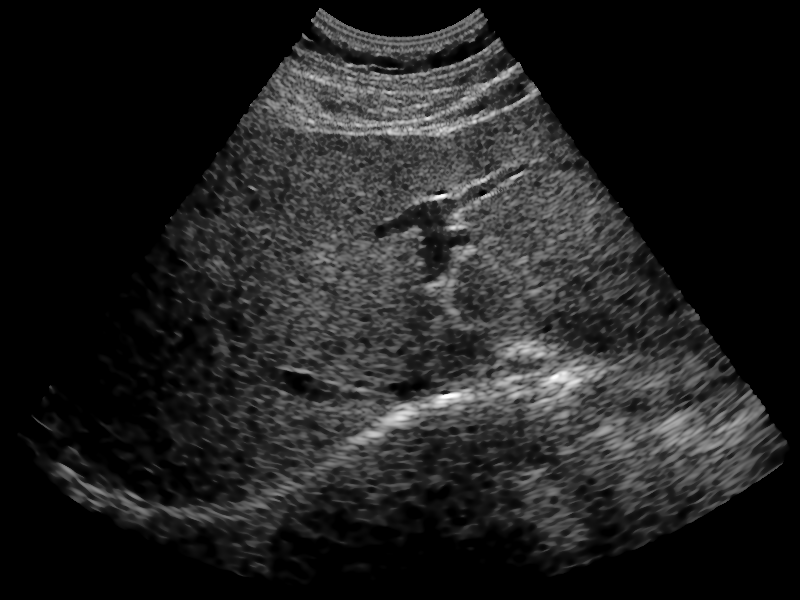
\includegraphics[width=\textwidth, trim={4cm 4cm 4cm 0cm}, clip]{figures/liver1_admss.png}};
      \spy on (0.15, 0.0) in node [redwindow, anchor=north] at ($(figA.south)$);
    \end{tikzpicture}
    \caption{ADMSS}\label{fig:liver1_admss}
  \end{subfigure}%
  \begin{subfigure}[b]{0.15\textwidth}
    \begin{tikzpicture}[
        spy using outlines={%
          rectangle, magnification=3,size=\textwidth,
          every spy on node/.append style={transparentwindow}
        }
      ]
      \node (figA) at (0.0,0.0) {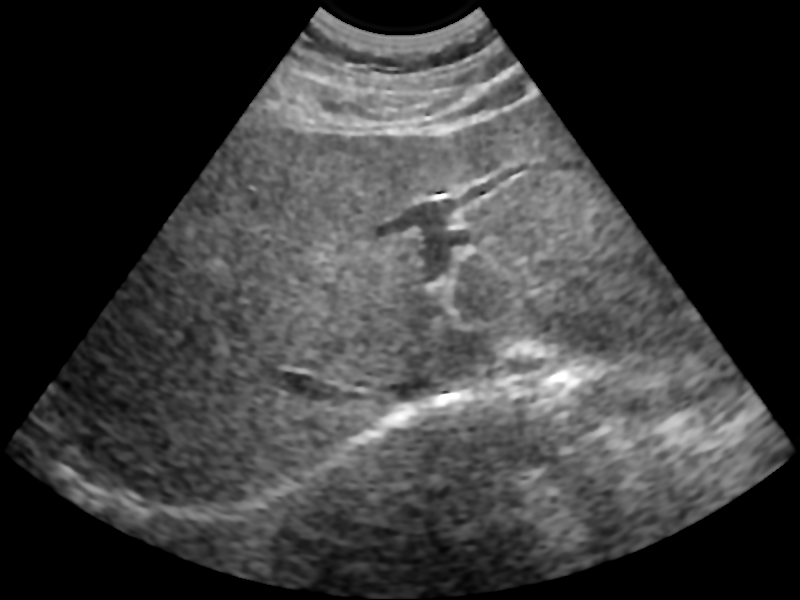
\includegraphics[width=\textwidth, trim={4cm 4cm 4cm 0cm}, clip]{figures/liver1_lpndsf.png}};
      \spy on (0.15, 0.0) in node [redwindow, anchor=north] at ($(figA.south)$);
    \end{tikzpicture}
    \caption{LPNDSF}\label{fig:liver1_lpndsf}
  \end{subfigure}%
  \begin{subfigure}[b]{0.15\textwidth}
    \begin{tikzpicture}[
        spy using outlines={%
          rectangle,magnification=3,size=\textwidth,
          every spy on node/.append style={transparentwindow}
        }
      ]
      \node (figA) at (0.0,0.0) {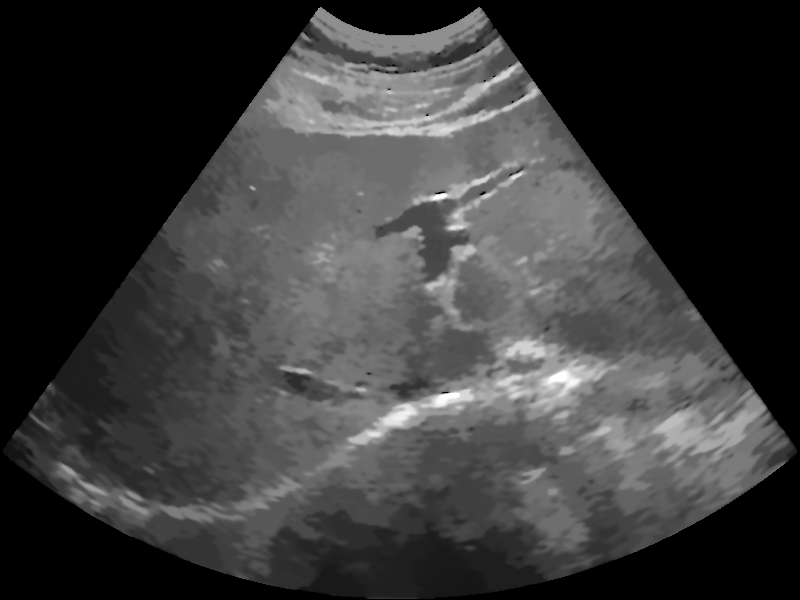
\includegraphics[width=\textwidth, trim={4cm 4cm 4cm 0cm}, clip]{figures/liver1_mnlm.png}};
      \spy on (0.15, 0.0) in node [redwindow, anchor=north] at ($(figA.south)$);
    \end{tikzpicture}
    \caption{MNLM}\label{fig:liver1_mnlm}
  \end{subfigure}%
  \begin{subfigure}[b]{0.15\textwidth}
    \begin{tikzpicture}[
        spy using outlines={%
          rectangle,magnification=3,size=\textwidth,
          every spy on node/.append style={transparentwindow}
        }
      ]
      \node (figA) at (0.0,0.0) {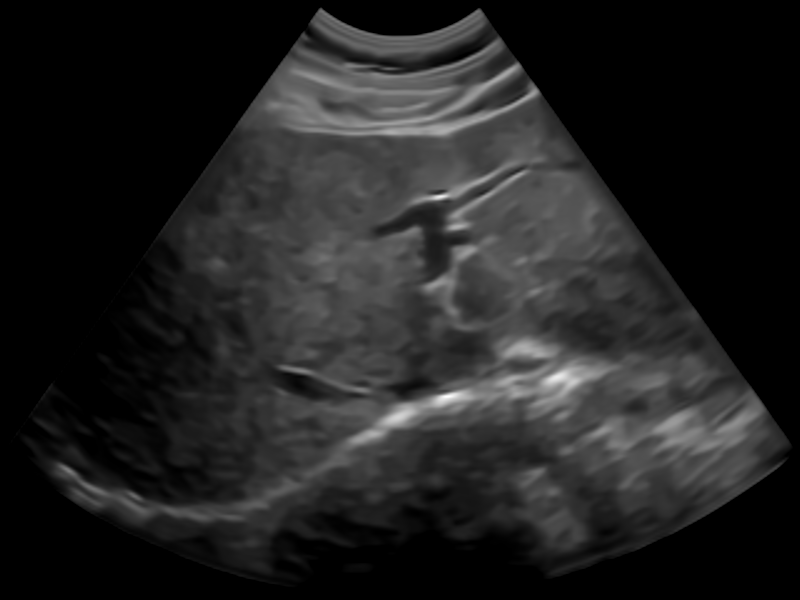
\includegraphics[width=\textwidth, trim={4cm 4cm 4cm 0cm}, clip]{figures/liver1_nllr.png}};
      \spy on (0.15, 0.0) in node [redwindow, anchor=north] at ($(figA.south)$);
    \end{tikzpicture}
    \caption{NLLR}\label{fig:liver1_nllr}
  \end{subfigure}%
  \begin{subfigure}[b]{0.15\textwidth}
    \begin{tikzpicture}[
        spy using outlines={%
          rectangle,magnification=3,size=\textwidth,
          every spy on node/.append style={transparentwindow}
        }
      ]
      \node (figA) at (0.0,0.0) {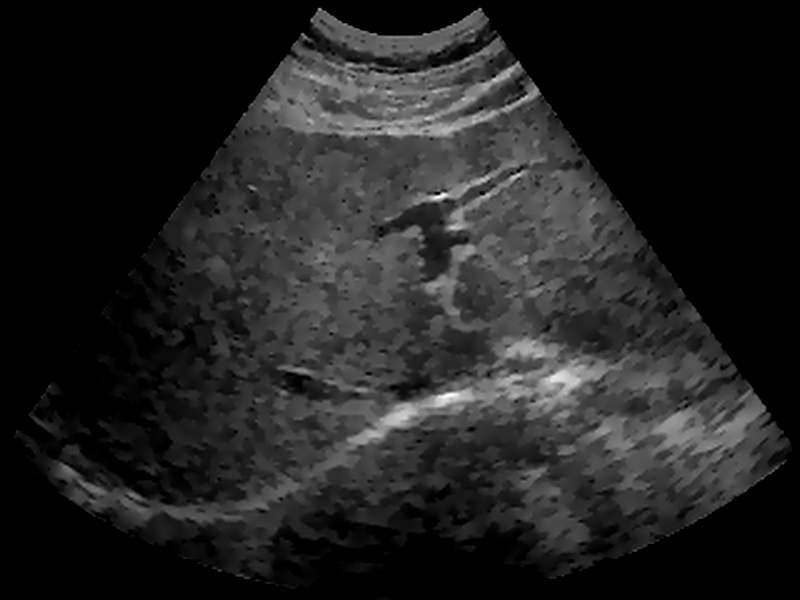
\includegraphics[width=\textwidth, trim={4cm 4cm 4cm 0cm}, clip]{figures/liver1_pfdtv.png}};
      \spy on (0.15, 0.0) in node [redwindow, anchor=north] at ($(figA.south)$);
    \end{tikzpicture}
    \caption{PFDTV}\label{fig:liver1_pfdtv}
  \end{subfigure}\\
  \begin{subfigure}[b]{0.15\textwidth}
    \begin{tikzpicture}[
        spy using outlines={%
          rectangle,magnification=3,size=\textwidth,
          every spy on node/.append style={transparentwindow}
        }
      ]
      \node (figA) at (0.0,0.0) {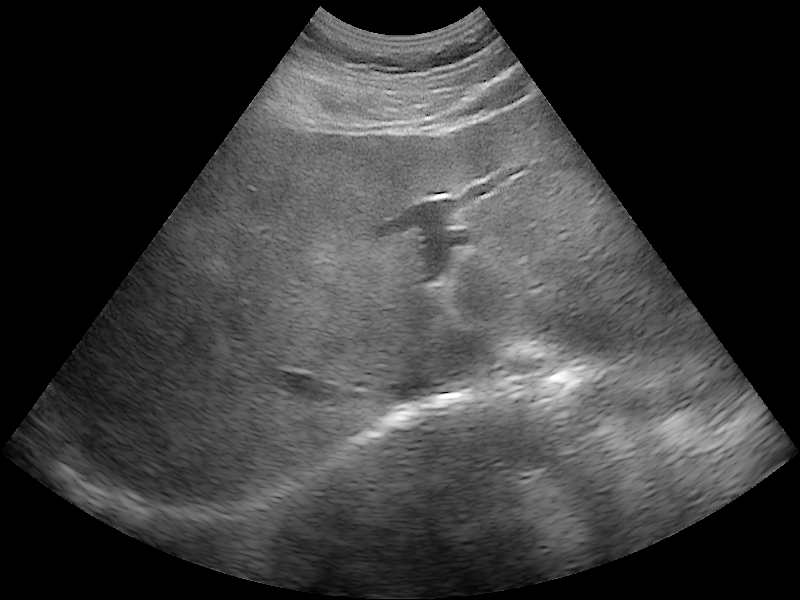
\includegraphics[width=\textwidth, trim={4cm 4cm 4cm 0cm}, clip]{figures/liver1_clpdQ.png}};
      \spy on (0.15, 0.0) in node [redwindow, anchor=north] at ($(figA.south)$);
    \end{tikzpicture}
    \caption{CLPD-SSNR}\label{fig:liver1_clpdssnr}
  \end{subfigure}%
  \begin{subfigure}[b]{0.15\textwidth}
    \begin{tikzpicture}[
        spy using outlines={%
          rectangle,magnification=3,size=\textwidth,
          every spy on node/.append style={transparentwindow}
        }
      ]
      \node (figA) at (0.0,0.0) {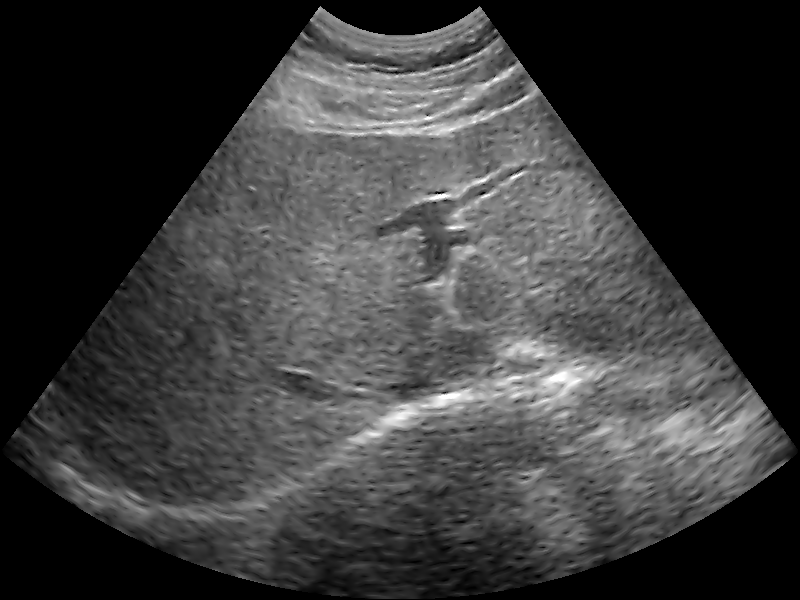
\includegraphics[width=\textwidth, trim={4cm 4cm 4cm 0cm}, clip]{figures/liver1_clpda.png}};
      \spy on (0.15, 0.0) in node [redwindow, anchor=north] at ($(figA.south)$);
    \end{tikzpicture}
    \caption{CLPD-A}\label{fig:liver1_clpda}
  \end{subfigure}%
  \begin{subfigure}[b]{0.15\textwidth}
    \begin{tikzpicture}[
        spy using outlines={%
          rectangle,magnification=3,size=\textwidth,
          every spy on node/.append style={transparentwindow}
        }
      ]
      \node (figA) at (0.0,0.0) {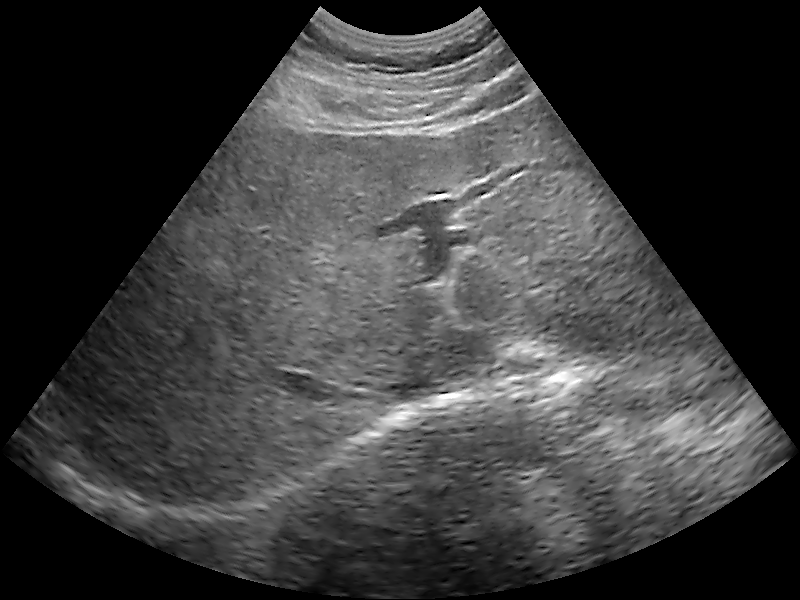
\includegraphics[width=\textwidth, trim={4cm 4cm 4cm 0cm}, clip]{figures/liver1_clpdb.png}};
      \spy on (0.15, 0.0) in node [redwindow, anchor=north] at ($(figA.south)$);
    \end{tikzpicture}
    \caption{CLPD-B}\label{fig:liver1_clpdb}
  \end{subfigure}%
  \begin{subfigure}[b]{0.15\textwidth}
    \begin{tikzpicture}[
        spy using outlines={%
          rectangle,magnification=3,size=\textwidth,
          every spy on node/.append style={transparentwindow}
        }
      ]
      \node (figA) at (0.0,0.0) {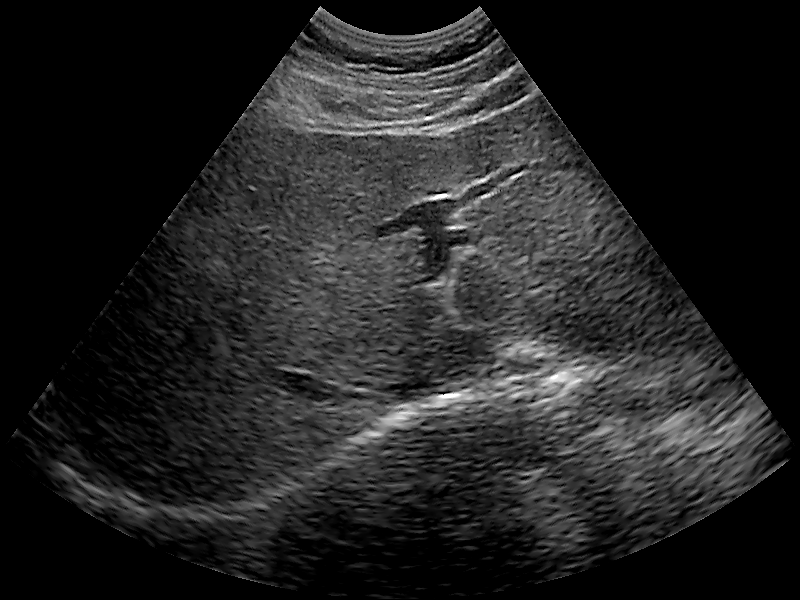
\includegraphics[width=\textwidth, trim={4cm 4cm 4cm 0cm}, clip]{figures/liver1_clpdc.png}};
      \spy on (0.15, 0.0) in node [redwindow, anchor=north] at ($(figA.south)$);
    \end{tikzpicture}
    \caption{CLPD-C}\label{fig:liver1_clpdc}
  \end{subfigure}%
  \begin{subfigure}[b]{0.15\textwidth}
    \begin{tikzpicture}[
        spy using outlines={%
          rectangle,magnification=3,size=\textwidth,
          every spy on node/.append style={transparentwindow}
        }
      ]
      \node (figA) at (0.0,0.0) {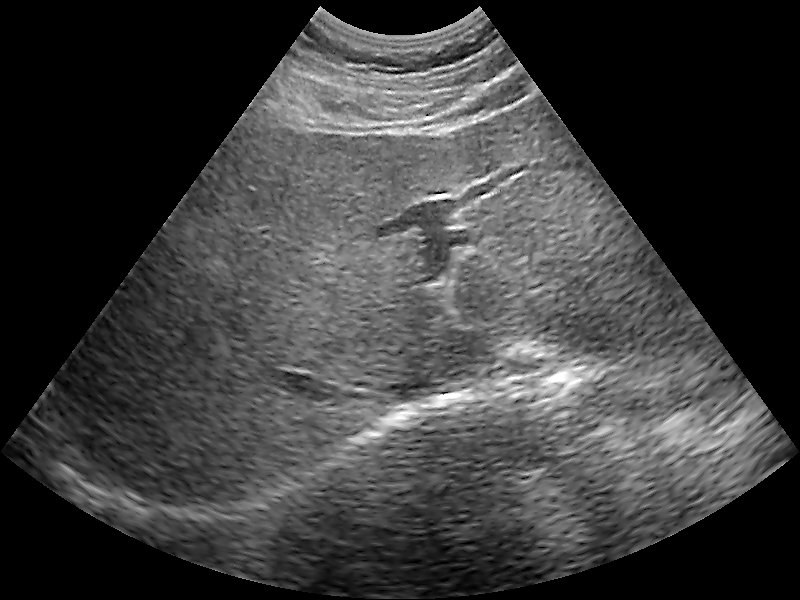
\includegraphics[width=\textwidth, trim={4cm 4cm 4cm 0cm}, clip]{figures/liver1_clpdd.png}};
      \spy on (0.15, 0.0) in node [redwindow, anchor=north] at ($(figA.south)$);
    \end{tikzpicture}
    \caption{CLPD-D}\label{fig:liver1_clpdd}
  \end{subfigure}%
  \begin{subfigure}[b]{0.15\textwidth}
    \begin{tikzpicture}[
        spy using outlines={%
          rectangle,magnification=3,size=\textwidth,
          every spy on node/.append style={redwindow}
        }
      ]
      \node (figA) at (0.0,0.0) {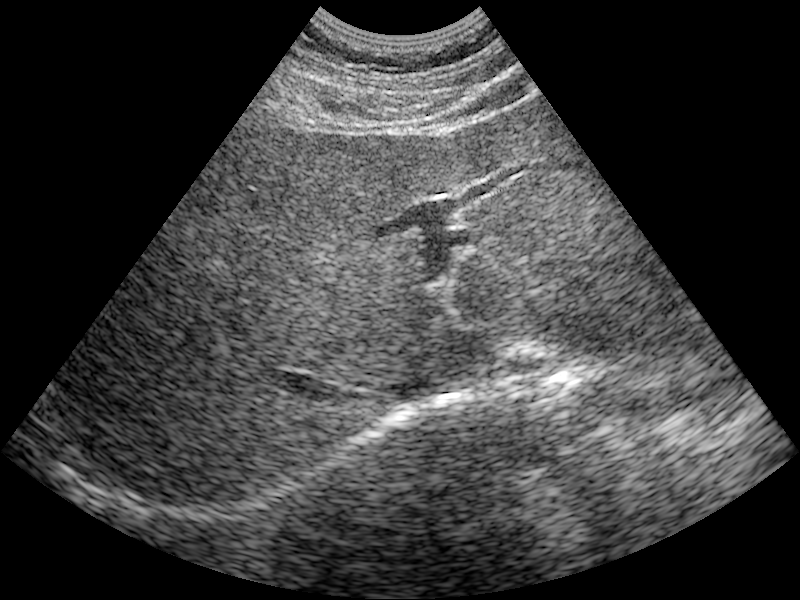
\includegraphics[width=\textwidth, trim={4cm 4cm 4cm 0cm}, clip]{figures/liver1.png}};
      \spy on (0.15, 0.0) in node [redwindow, anchor=north] at ($(figA.south)$);
    \end{tikzpicture}
    \caption{Original}\label{fig:liver_original}
  \end{subfigure}
  \caption{Results on a liver subcostal-view image.}\label{fig:liver1}
\end{figure*}

%%% Local Variables:
%%% TeX-master: "master"
%%% End:

%
\paragraph{Contrast-to-Noise Ratio (CNR)}
The CNR first introduced by Patterson and Foster~\cite{patterson_improvement_1983} measures the mean response difference of two regions-of-interests relative to their standard deviations such as
\begin{align}
  \mathrm{CNR} \texttt{[dB]} = 10 \log_{10} \left(\,| \mu_{1} - \mu_{2} | \,/\, \sqrt{\sigma^2_1 + \sigma^2_2}\, \right)
\end{align}
where \(\mu_1, \mu_2\) are the mean responses of the regions-of-interests, and \(\sigma_1, \sigma_2\) are their standard deviations, respectively.
While the CNR is loosely related to the lesions detectibility~\cite{smith_ultrasound_1984}, Rindal \textit{et al.} has shown that it is less reliable when the dynamic range is altered~\cite{rindal_effect_2019}.
We present the CNR in decibel scale.

%% Nonetheless, the CNR still provides a measure of relative contrast.

\paragraph{Generalized CNR (gCNR)}
As a remedy to the limitations of the CNR, Rodriguez-Molares \textit{et al.}~\cite{rodriguez-molares_generalized_2020} proposed the gCNR metric.
They showed that it is less affected by dynamic range alternations, making it a better general performance metric.
The gCNR is defined as
\begin{align}
  \text{gCNR} = 1 - \int_{-\infty}^{\infty} \min\big(p_1\left(x\right), p_2\left(x\right)\big) \, dx
\end{align}
where \(p_1\left(x\right)\) and \(p_2\left(x\right)\) are the probability densities of \(x\) subject to the pixel intensity distributions of the regions-of-interests 1 and 2.

\paragraph{Structural Similarity Index (SSIM)}
The SSIM is a metric for measuring the \textit{structural} similarity of images, which is derived as a product of the differences in lumiance, structure, and contrast~\cite{wang_image_2004a}.
Wang \textit{et al.} has shown that the SSIM is aligned with the perception of humans, and is sensitive to distortions such as blur and blockiness.
Mathematically, the SSIM between image 1 and 2 is computed such that
\begin{align}
  \mathrm{SSIM} = \frac{1}{N} \sum_k^N \frac{
    (2 \mu_{1,k} \, \mu_{2, k} + C_1)\,(2 \sigma_{12, k} + C_2)
  }{
    (\mu_{1,k}^2 + \mu_{2,k}^2 + C_1)\,( \sigma_{1,k}^2 + \sigma_{2,k}^2 + C_2)
  }
\end{align}
where \(\mu_{1,k}\), \(\mu_{2,k}\), are the mean of the \(k\)th patch on each images, \(\sigma_{1,k}^2\), \(\sigma_{2,k}^2\) are their respective variances, and \(\sigma_{12, k}\) is the covariance of the two.
The SSIM is taken as an average over all the patches, which are taken by a \(11 \times 11\) Gaussian window of standard deviation 1.5.
The coefficients are chosen as \(C_1 = 1 \times 10^{-4}, C_2 = 9 \times 10^{-4} \).
We use the implementation of the \texttt{ImageQualityIndexes.jl} library\footnote{\url{https://github.com/JuliaImages/ImageQualityIndexes.jl}}

\paragraph{\(S_3\) Index}
Finally, we use a metric for evaluating the blurriness of the images.
Blurriness metrics have not been traditionally used for evaluating the quality of medical ultrasound images.
But, we will later show that blurriness is an important quality factor for sonographers.
In this work, we use the \(S_3\) metric proposed in~\cite{vu_bf_2012}.
The \(S_3\) value of the \(k\)th patch is defined as a harmonic mean such that
\begin{align}
  S_3\left(k\right) = \sqrt{S_1\left(k\right)} \sqrt{S_2\left(k\right)}
\end{align}
where \(S_1\left(k\right)\) and \(S_2\left(k\right)\) are its spatial and spectral measures of sharpness.
The final \(S_3\) index of an image is given as the average of the top 1\% \(S_3\) values.
We use the official implementation\footnote{\url{https://sites.google.com/site/cuongvt101/research/Sharpness-measure}}.

%
\begin{figure}[h]
  \centering
  \subfloat[Liver image]{
    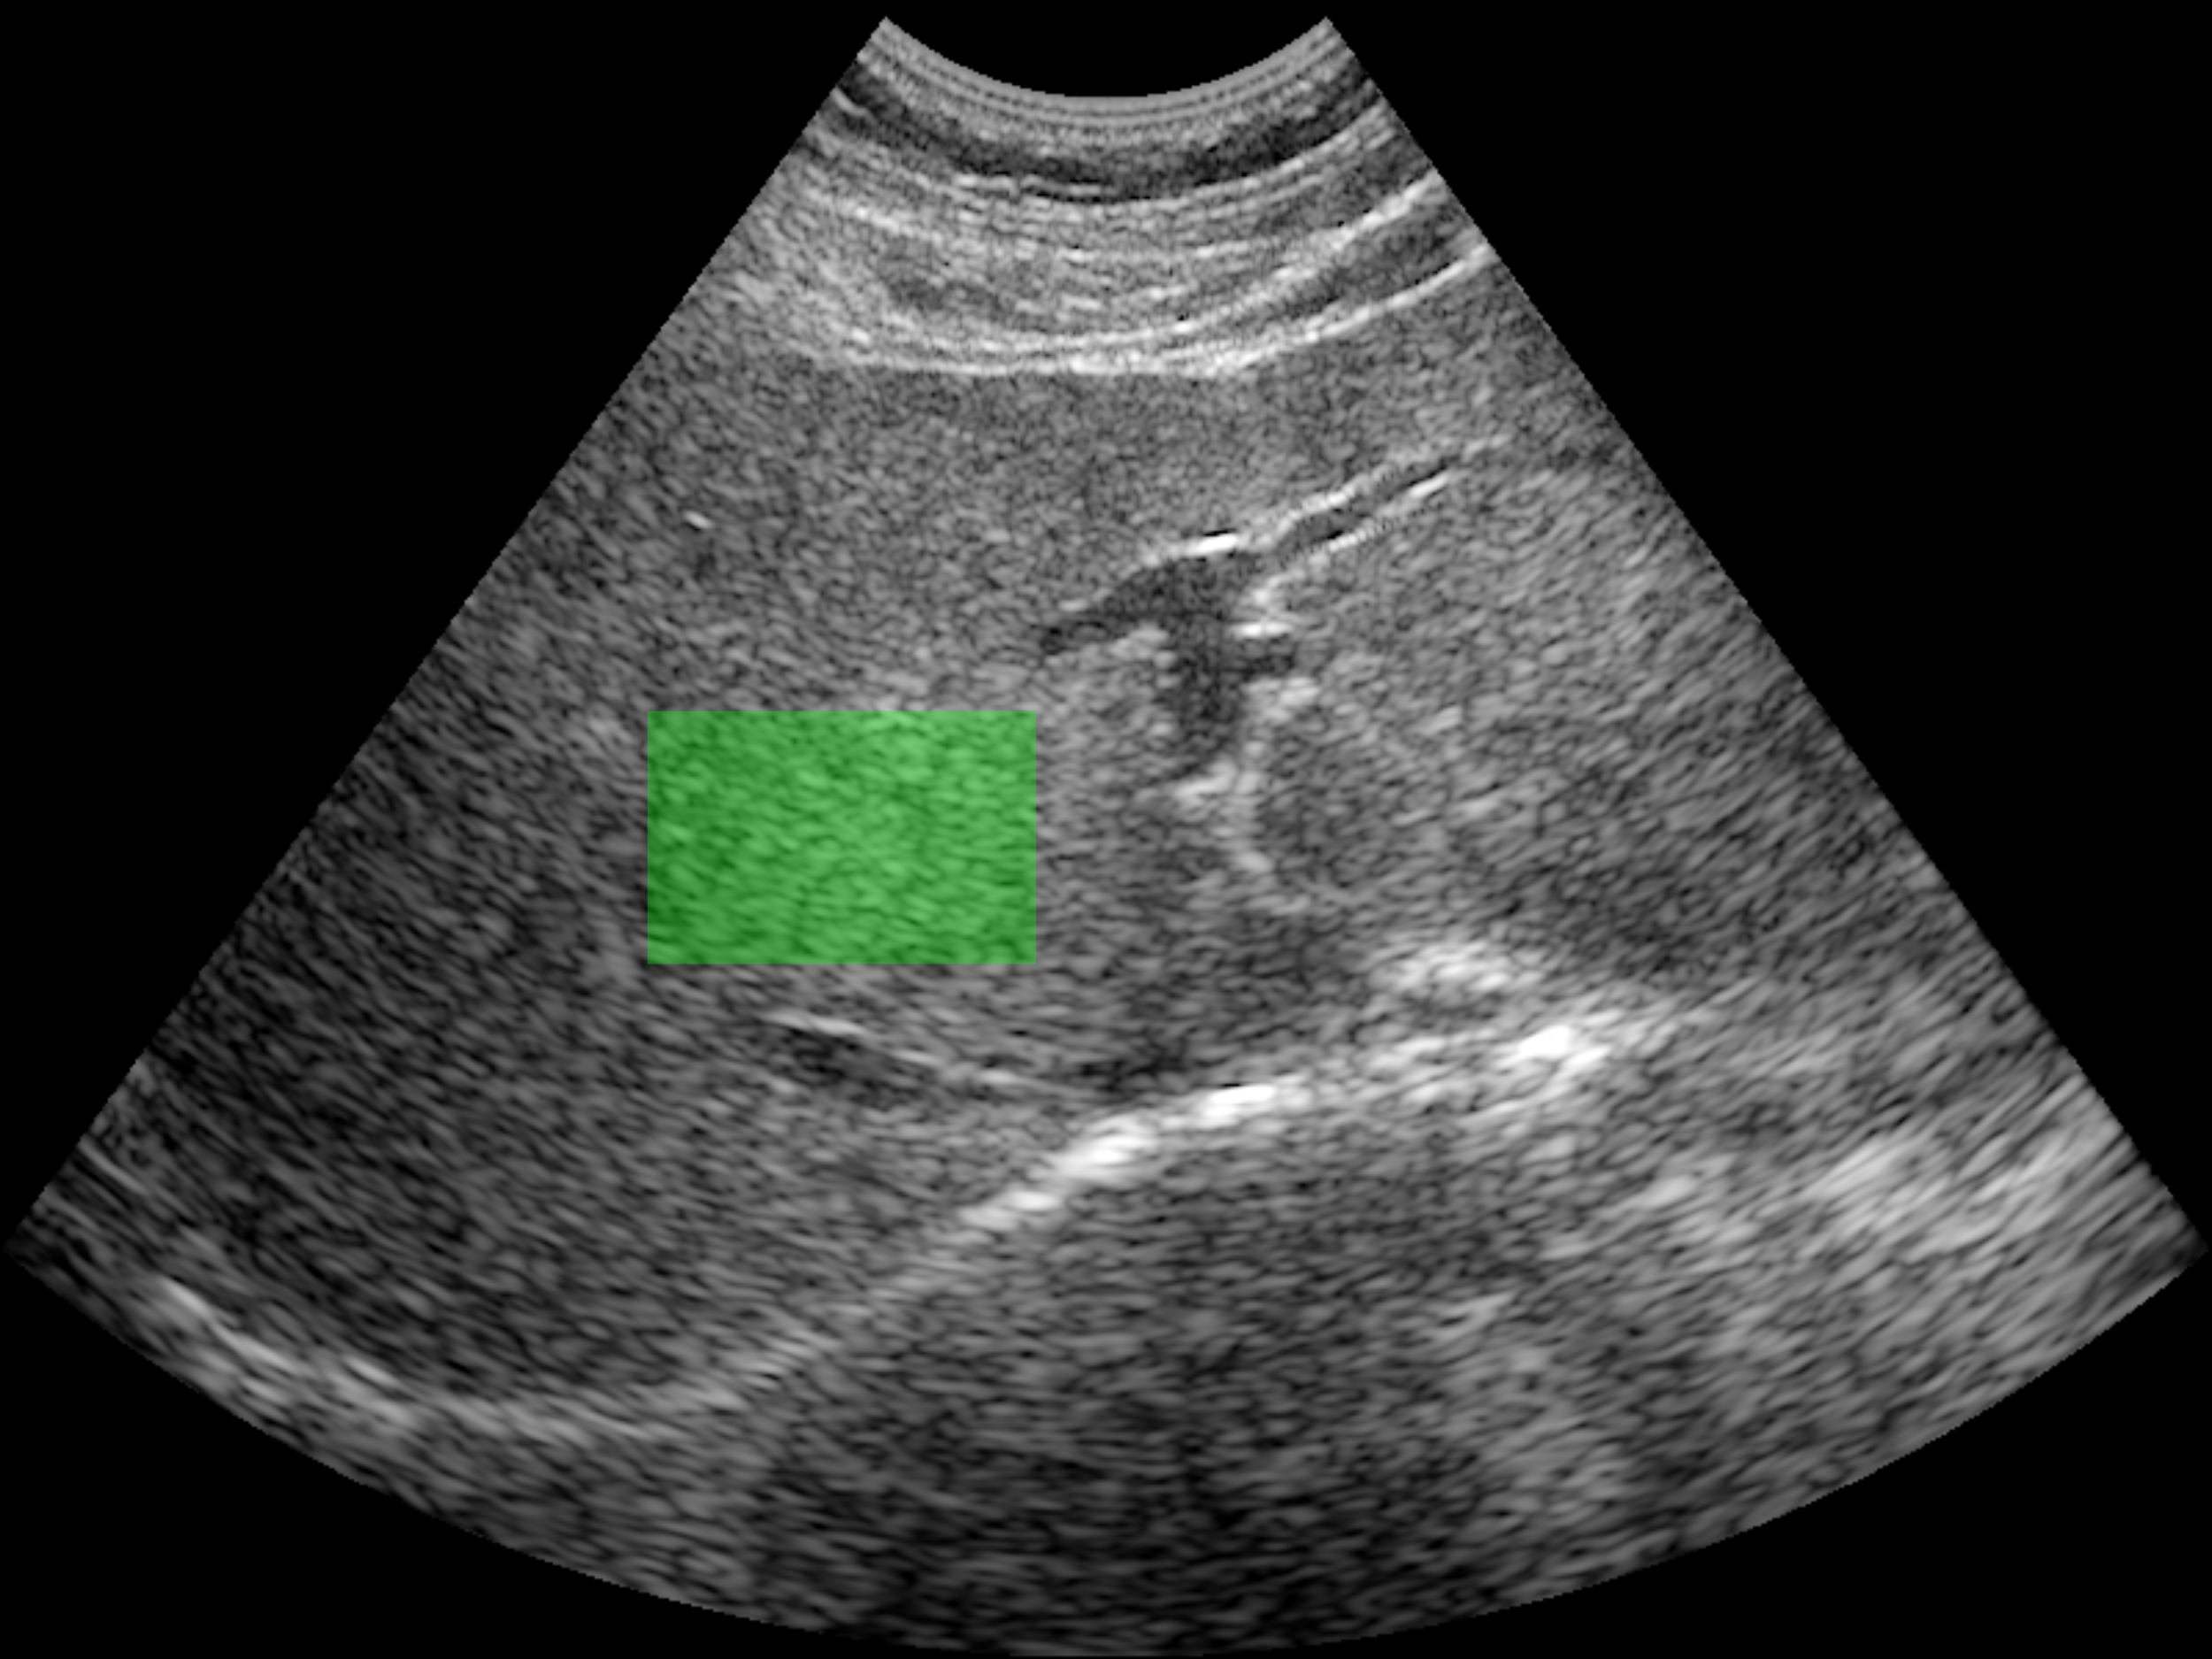
\includegraphics[height=2.5cm]{figures/liver_roi.png}\label{fig:liver_roi}
  }
  \subfloat[Cardiac image]{
    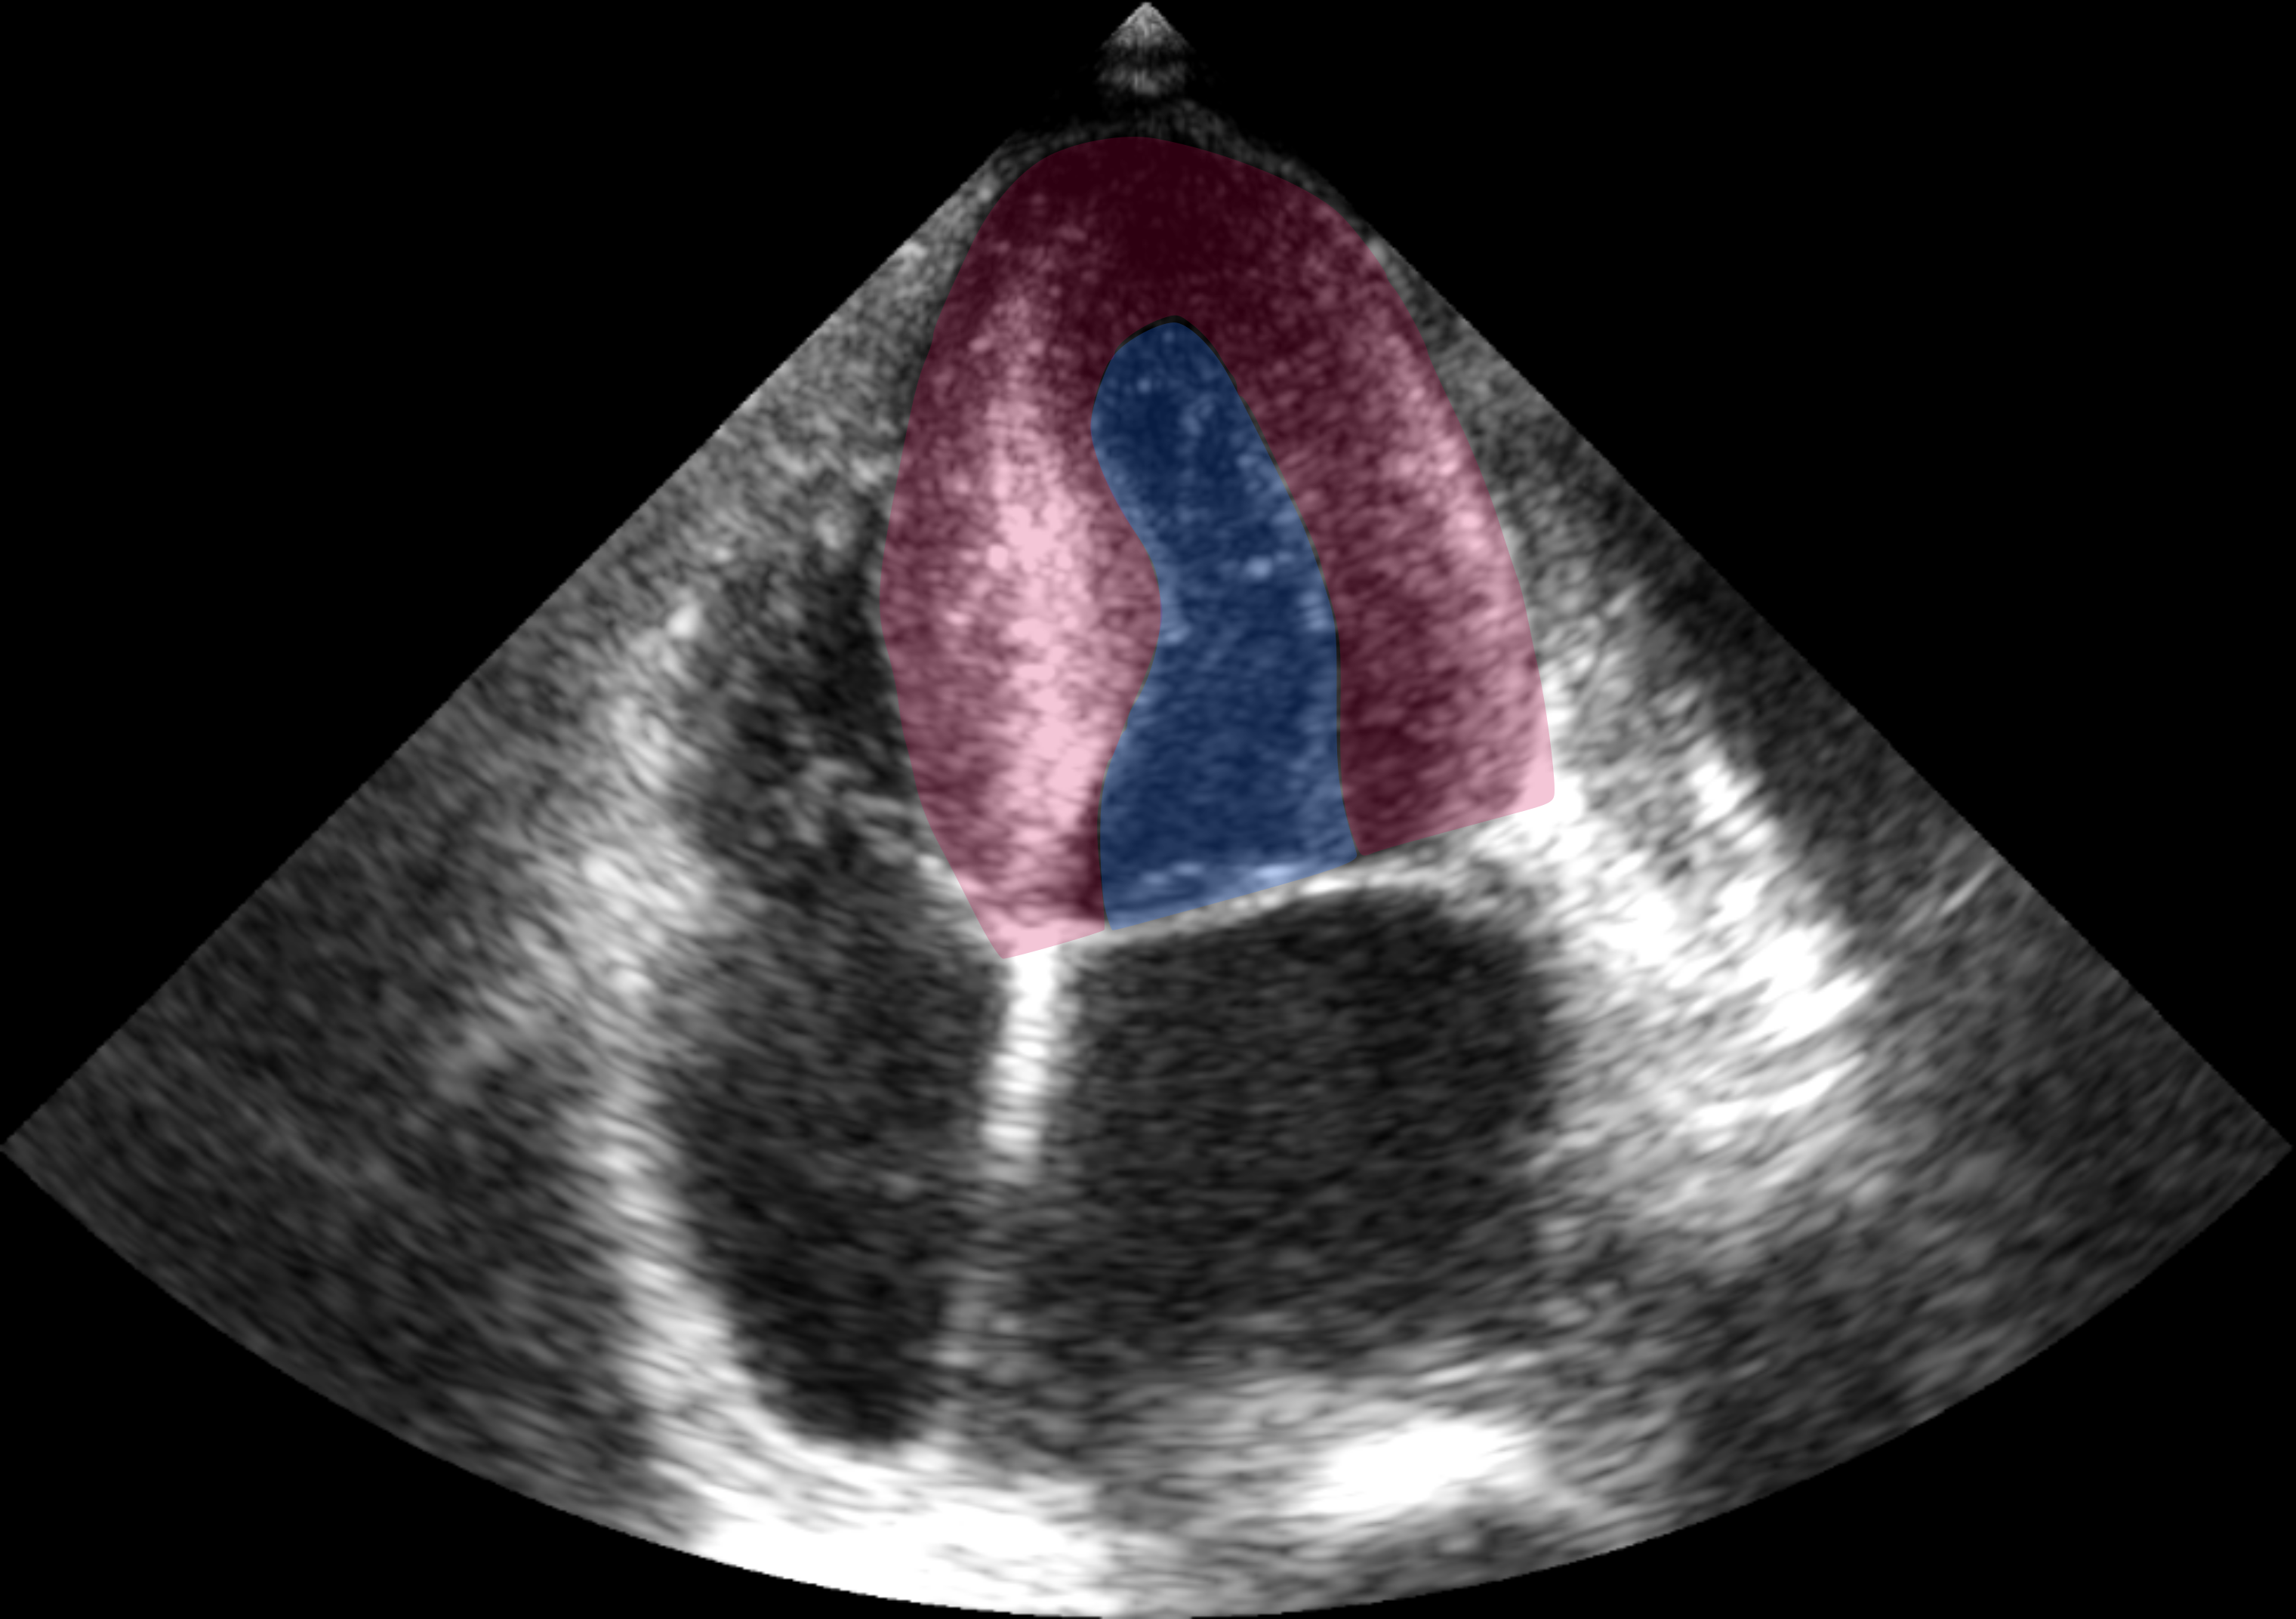
\includegraphics[height=2.5cm]{figures/cardiac_roi.png}\label{fig:cardiac_roi}
  }
  \caption{Regions-of-interests used for using the objective performance metrics.
    (a) The \textcolor{orange}{orange} region is used for computing the SSNR.
    (b) The \textcolor{red}{red} region (endocardium of the left ventricle) and \textcolor{blue}{blue} region (blood of the left ventricle) are used for computing the gCNR and CNR.
    The red region is also used for computing the SNR.
  }\label{fig:roi}
\end{figure}
% 
%\paragraph{Regions-of-Interests}
The regions-of-interests used for computing the performance metrics are shown in~\cref{fig:roi}.
For the liver image, we compute the metrics over multiple frames, while for the echocardiographic image, we compute the metrics only using the presented frame.


\begin{figure*}
  \vspace{-0.2in}
  \centering
  \begin{subfigure}[b]{0.15\textwidth}
    \begin{tikzpicture}[
        spy using outlines={%
          rectangle,magnification=3,size=\textwidth,
          every spy on node/.append style={transparentwindow}
        }
      ]
      \node (figA) at (0.0,0.0) {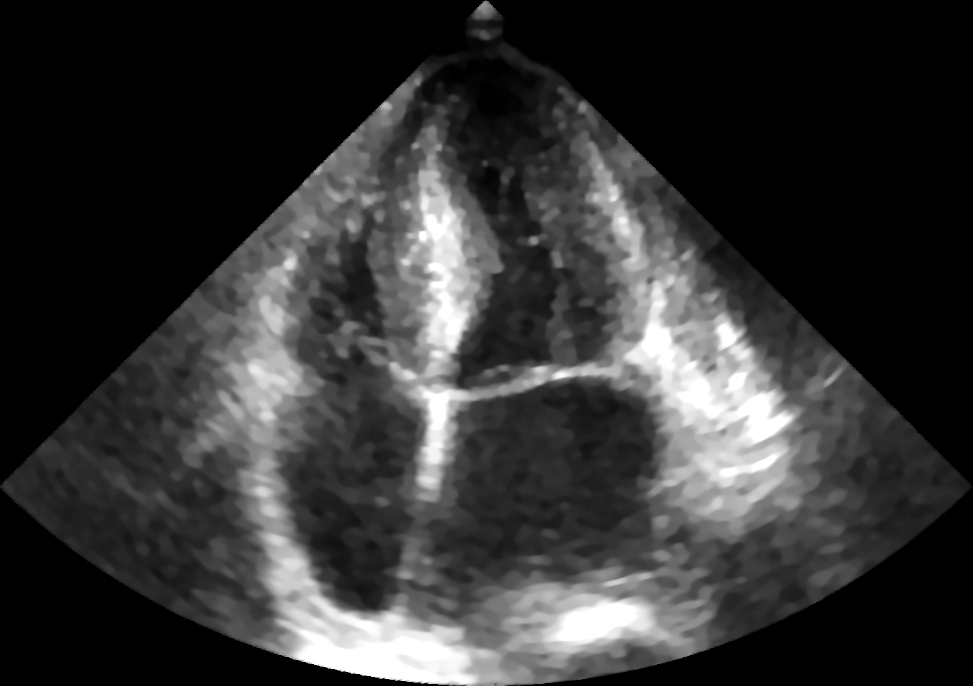
\includegraphics[width=\textwidth]{figures/cardiac3_osrad.png}};
      \spy on (0.1, 0.2) in node [redwindow, anchor=north] at ($(figA.south)$);
    \end{tikzpicture}
    \caption{OSRAD}
  \end{subfigure}%
  \begin{subfigure}[b]{0.15\textwidth}
    \begin{tikzpicture}[
        spy using outlines={%
          rectangle, magnification=3,size=\textwidth,
          every spy on node/.append style={transparentwindow}
        }
      ]
      \node (figA) at (0.0,0.0) {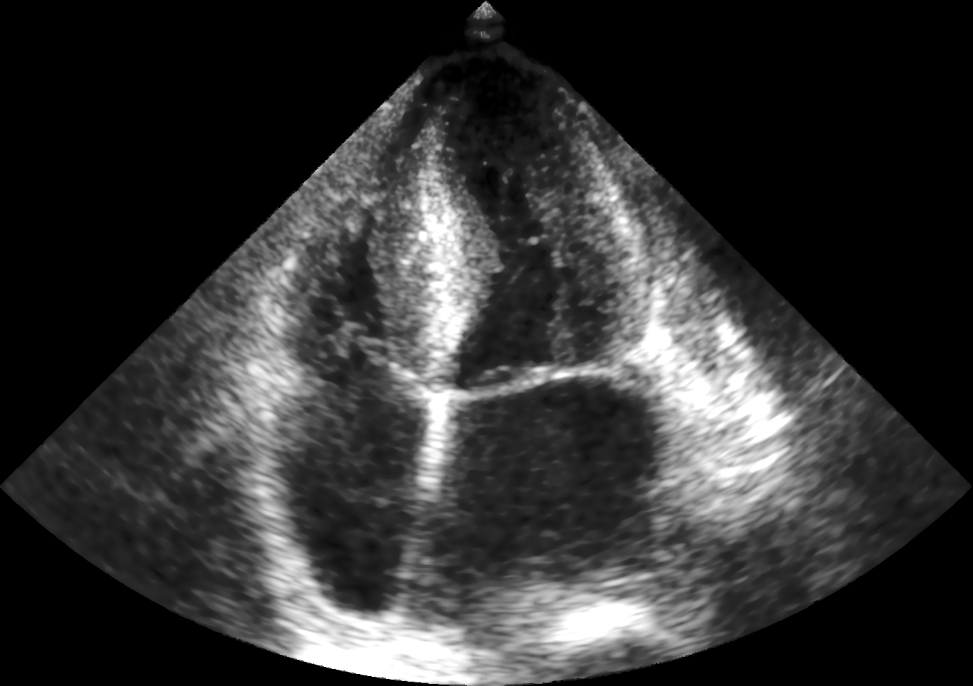
\includegraphics[width=\textwidth]{figures/cardiac3_admss.png}};
      \spy on (0.1, 0.2) in node [redwindow, anchor=north] at ($(figA.south)$);
    \end{tikzpicture}
    \caption{ADMSS}
  \end{subfigure}%
  \begin{subfigure}[b]{0.15\textwidth}
    \begin{tikzpicture}[
        spy using outlines={%
          rectangle, magnification=3,size=\textwidth,
          every spy on node/.append style={transparentwindow}
        }
      ]
      \node (figA) at (0.0,0.0) {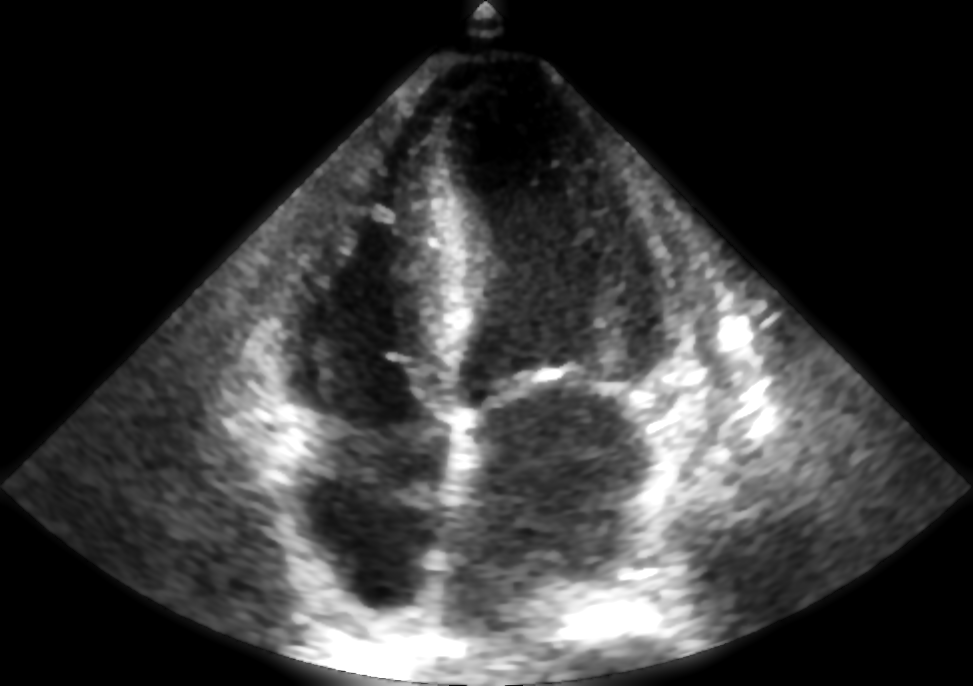
\includegraphics[width=\textwidth]{figures/cardiac3_lpndsf.png}};
      \spy on (0.1, 0.2) in node [redwindow, anchor=north] at ($(figA.south)$);
    \end{tikzpicture}
    \caption{LPNDSF}
  \end{subfigure}%
  \begin{subfigure}[b]{0.15\textwidth}
    \begin{tikzpicture}[
        spy using outlines={%
          rectangle,magnification=3,size=\textwidth,
          every spy on node/.append style={transparentwindow}
        }
      ]
      \node (figA) at (0.0,0.0) {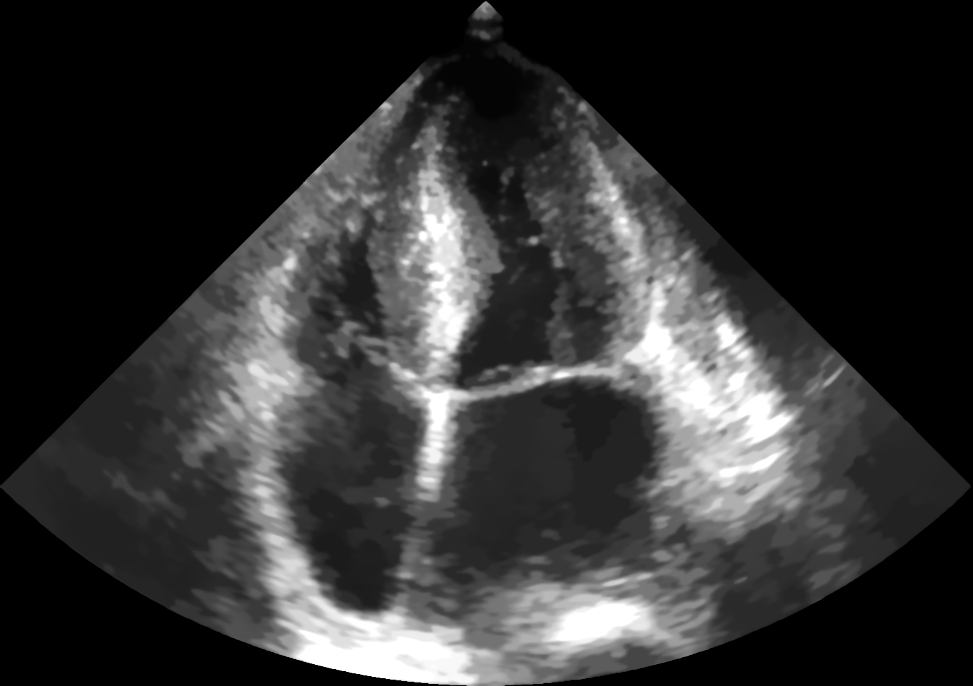
\includegraphics[width=\textwidth]{figures/cardiac3_mnlm.png}};
      \spy on (0.1, 0.2) in node [redwindow, anchor=north] at ($(figA.south)$);
    \end{tikzpicture}
    \caption{MNLM}
  \end{subfigure}%
  \begin{subfigure}[b]{0.15\textwidth}
    \begin{tikzpicture}[
        spy using outlines={%
          rectangle,magnification=3,size=\textwidth,
          every spy on node/.append style={transparentwindow}
        }
      ]
      \node (figA) at (0.0,0.0) {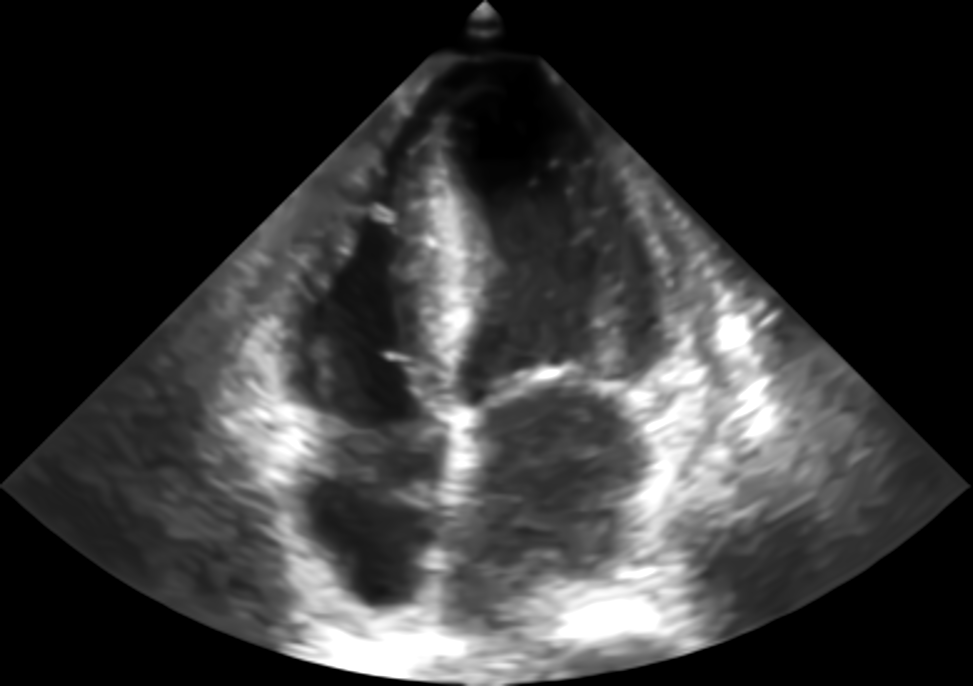
\includegraphics[width=\textwidth]{figures/cardiac3_nllr.png}};
      \spy on (0.1, 0.2) in node [redwindow, anchor=north] at ($(figA.south)$);
    \end{tikzpicture}
    \caption{NLLR}
  \end{subfigure}%
  \begin{subfigure}[b]{0.15\textwidth}
    \begin{tikzpicture}[
        spy using outlines={%
          rectangle,magnification=3,size=\textwidth,
          every spy on node/.append style={transparentwindow}
        }
      ]
      \node (figA) at (0.0,0.0) {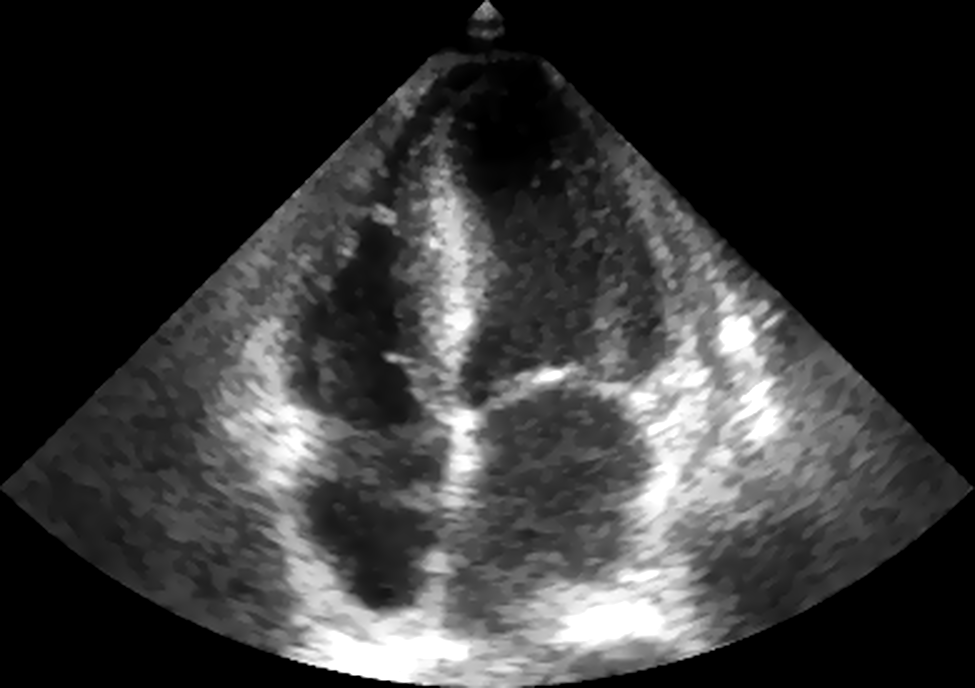
\includegraphics[width=\textwidth]{figures/cardiac3_pfdtv.png}};
      \spy on (0.1, 0.2) in node [redwindow, anchor=north] at ($(figA.south)$);
    \end{tikzpicture}
    \caption{PFDTV}
  \end{subfigure}\\
  %% \begin{subfigure}[b]{0.15\textwidth}
  %%   \begin{tikzpicture}[
  %%       spy using outlines={%
  %%         rectangle,magnification=3,size=\textwidth,
  %%         every spy on node/.append style={transparentwindow}
  %%       }
  %%     ]
  %%     \node (figA) at (0.0,0.0) {\includegraphics[width=\textwidth, trim={4cm 4cm 4cm 0cm}, clip]{figures/cardiac3_clpdQ.png}};
  %%     \spy on (0.1, 0.2) in node [redwindow, anchor=north] at ($(figA.south)$);
  %%   \end{tikzpicture}
  %%   \caption{CLPD-SSNR}
  %% \end{subfigure}%
  \begin{subfigure}[b]{0.15\textwidth}
    \begin{tikzpicture}[
        spy using outlines={%
          rectangle,magnification=3,size=\textwidth,
          every spy on node/.append style={transparentwindow}
        }
      ]
      \node (figA) at (0.0,0.0) {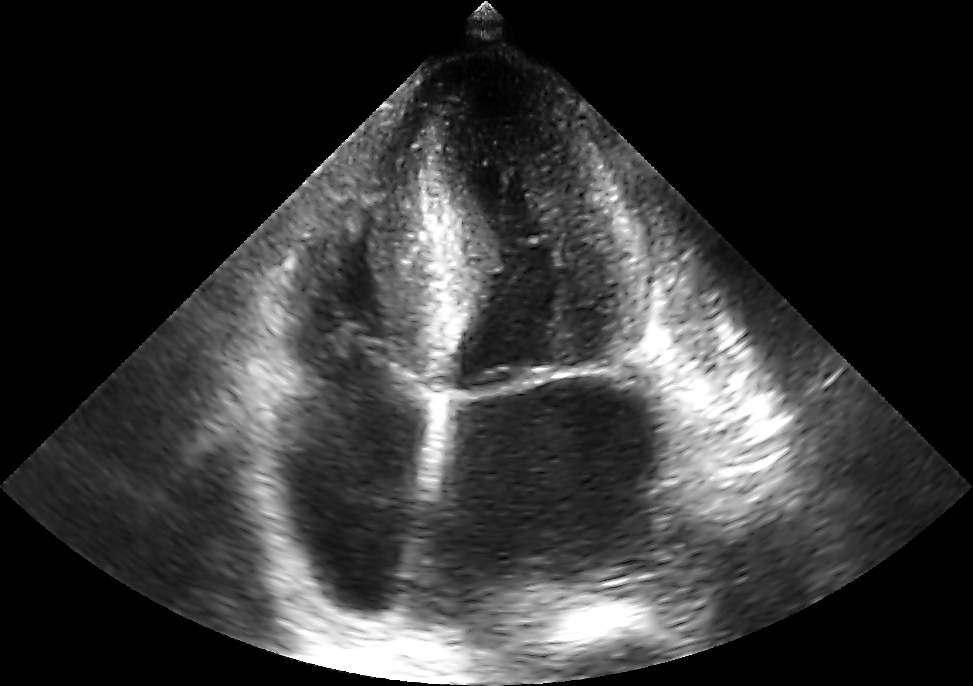
\includegraphics[width=\textwidth]{figures/cardiac3_clpda.png}};
      \spy on (0.1, 0.2) in node [redwindow, anchor=north] at ($(figA.south)$);
    \end{tikzpicture}
    \caption{CLPD-A}
  \end{subfigure}%
  \begin{subfigure}[b]{0.15\textwidth}
    \begin{tikzpicture}[
        spy using outlines={%
          rectangle,magnification=3,size=\textwidth,
          every spy on node/.append style={transparentwindow}
        }
      ]
      \node (figA) at (0.0,0.0) {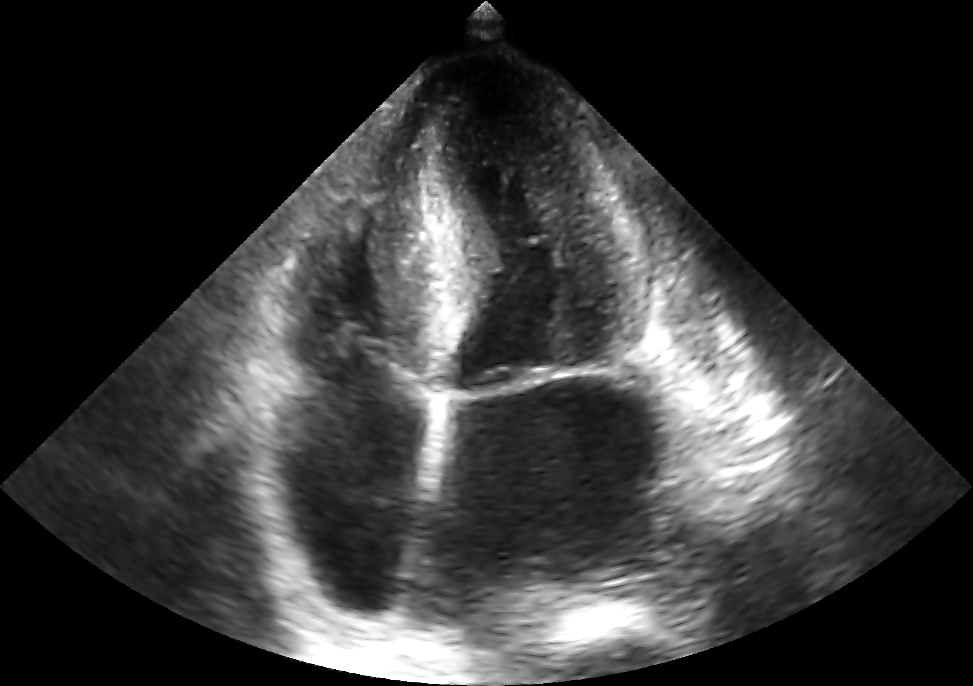
\includegraphics[width=\textwidth]{figures/cardiac3_clpdb.png}};
      \spy on (0.1, 0.2) in node [redwindow, anchor=north] at ($(figA.south)$);
    \end{tikzpicture}
    \caption{CLPD-B}
  \end{subfigure}%
  \begin{subfigure}[b]{0.15\textwidth}
    \begin{tikzpicture}[
        spy using outlines={%
          rectangle,magnification=3,size=\textwidth,
          every spy on node/.append style={transparentwindow}
        }
      ]
      \node (figA) at (0.0,0.0) {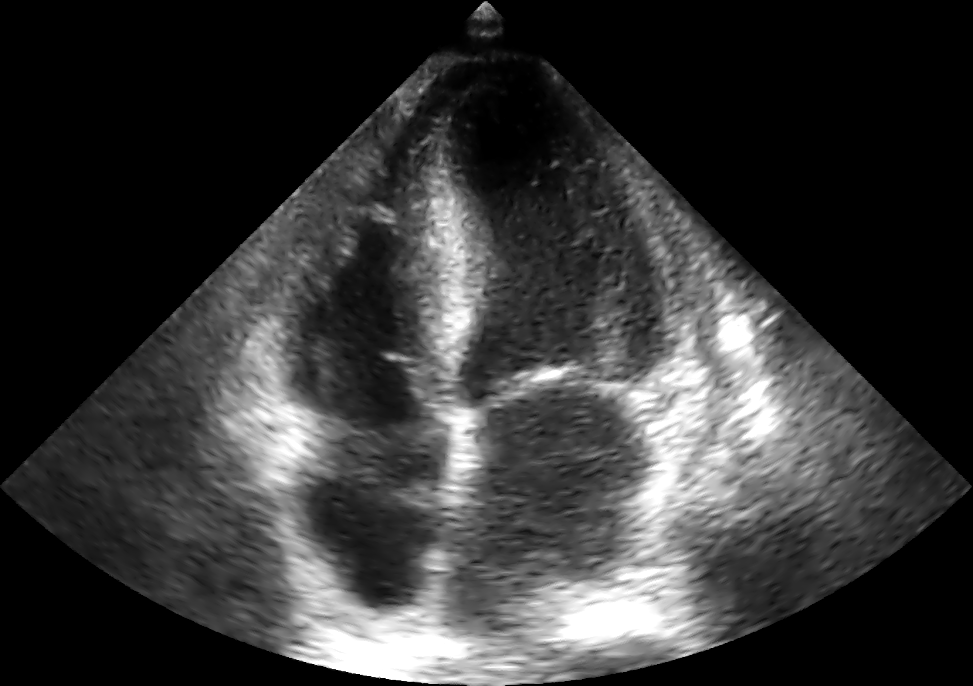
\includegraphics[width=\textwidth]{figures/cardiac3_clpde.png}};
      \spy on (0.1, 0.2) in node [redwindow, anchor=north] at ($(figA.south)$);
    \end{tikzpicture}
    \caption{CLPD-E}
  \end{subfigure}%
  \begin{subfigure}[b]{0.15\textwidth}
    \begin{tikzpicture}[
        spy using outlines={%
          rectangle,magnification=3,size=\textwidth,
          every spy on node/.append style={transparentwindow}
        }
      ]
      \node (figA) at (0.0,0.0) {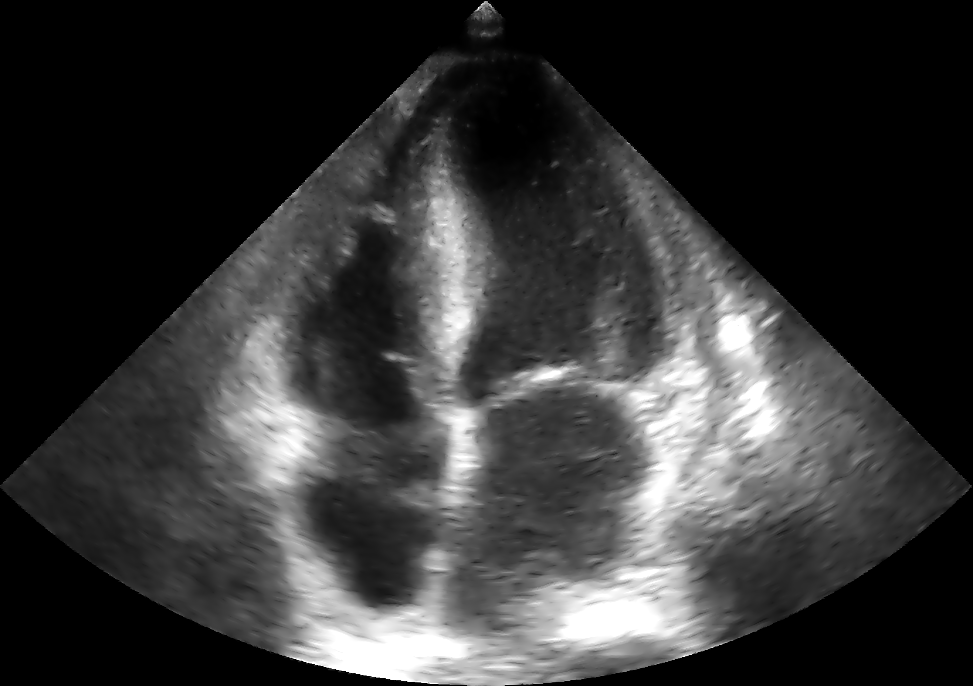
\includegraphics[width=\textwidth]{figures/cardiac3_clpdf.png}};
      \spy on (0.1, 0.2) in node [redwindow, anchor=north] at ($(figA.south)$);
    \end{tikzpicture}
    \caption{CLPD-F}
  \end{subfigure}%
  \begin{subfigure}[b]{0.15\textwidth}
    \begin{tikzpicture}[
        spy using outlines={%
          rectangle,magnification=3,size=\textwidth,
          every spy on node/.append style={redwindow}
        }
      ]
      \node (figA) at (0.0,0.0) {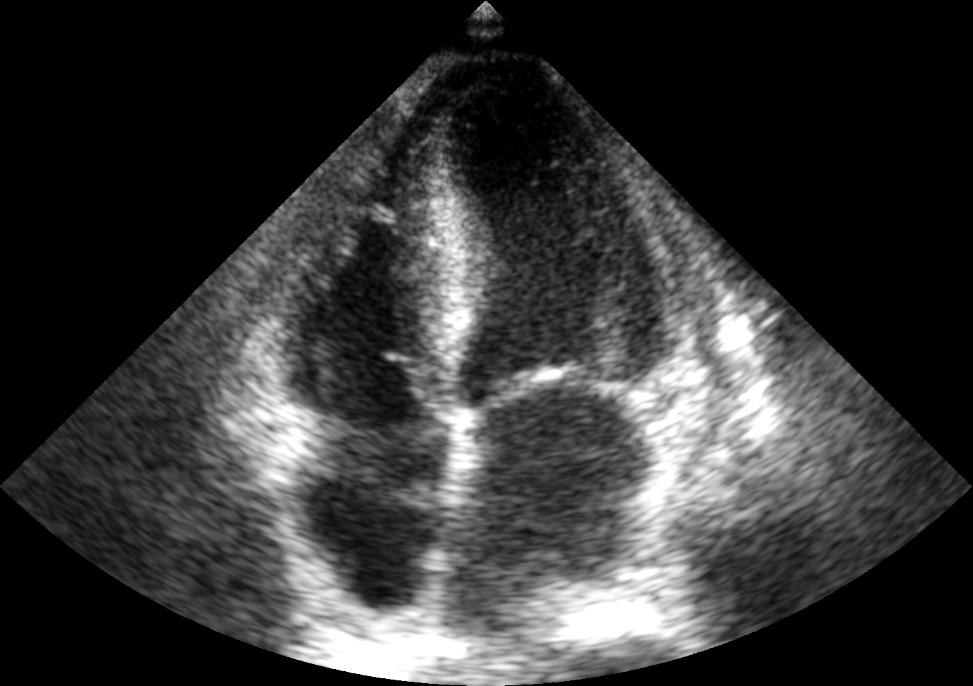
\includegraphics[width=\textwidth]{figures/cardiac3.png}};
      \spy on (0.1, 0.2) in node [redwindow, anchor=north] at ($(figA.south)$);
    \end{tikzpicture}
    \caption{Original}\label{fig:cardiac3_original}
  \end{subfigure}
  \caption{
    Results on echocardiographic 4-chamber view.
    The red squares are zooming on the left-ventricle.
  }\label{fig:cardiac3}
  \vspace{-0.15in}
\end{figure*}

%
\begin{table}
  \centering
  \caption{Quantatitive Results on a Liver Subcostal View}\label{table:liver1}
  \begin{threeparttable}
  \setlength{\tabcolsep}{3.5pt}
  \begin{tabular}{llrrr}
    \toprule
    & \multicolumn{1}{c}{\textbf{Algorithm}}
    & \multicolumn{1}{c}{\textbf{SSNR} \texttt{[dB]}}
    & \multicolumn{1}{c}{\textbf{SSIM}}
    & \multicolumn{1}{c}{\(\mathbf{S_{3}}\)} \\\midrule
    \multirow{6}{*}{\footnotesize{Baselines}} & OSRAD & \textbf{20.8 {\tiny(20.3, 21.2)}} & 0.792 {\tiny(0.791, 0.794)} & 0.476 {\tiny(0.473, 0.481)}\\
    & ADMSS & 16.9 {\tiny(16.5, 17.4)} & \textbf{0.927 {\tiny(0.893, 0.963)}} & 0.350 {\tiny(0.347, 0.353)} \\
    & LPNDSF & 19.7 {\tiny(19.4, 20.0)} & 0.763 {\tiny(0.762, 0.764)}         & 0.343 {\tiny(0.340, 0.346)} \\
    & MNLM & \textbf{22.1 {\tiny(21.6, 22.7)}} & 0.811 {\tiny(0.809, 0.812)}  & 0.033 {\tiny(0.329, 0.342)} \\
    & NLLR & \textbf{22.0 {\tiny(21.6, 22.5)}} & 0.764 {\tiny(0.762, 0.765)}  & 0.141 {\tiny(0.140, 0.142)} \\
    & PFDTV & \textbf{20.0 {\tiny(19.6, 20.4)}} & 0.822 {\tiny(0.820, 0.823)} & 0.461 {\tiny(0.456, 0.465)} \\
    \midrule
    \multirow{5}{*}{\footnotesize{This work}} & CLPD-{\scriptsize{SSNR}}  & \textbf{21.0 {\tiny(20.7, 21.4)}} & \textbf{0.914 {\tiny(0.913, 0.914)}} & \textbf{0.509 {\tiny(0.507, 0.511)}} \\
    & CLPD-A  & 19.9 {\tiny(19.6, 20.2)} & 0.883 {\tiny(0.882, 0.884)} & \textbf{0.490 {\tiny(0.486, 0.494)}} \\
    & CLPD-B  & 19.8 {\tiny(19.6, 20.2)} & \textbf{0.913 {\tiny(0.913, 0.914)}} & \textbf{0.507 {\tiny(0.503, 0.511)}} \\
    & CLPD-C  & 18.2 {\tiny(18.0, 18.5)} & \textbf{0.954 {\tiny(0.953, 0.954)}} & \textbf{0.587 {\tiny(0.581, 0.592)}} \\
    & CLPD-D & 19.0 {\tiny(18.7, 19.3)} & \textbf{0.933 {\tiny(0.932, 0.933)}} &  \textbf{0.565 {\tiny(0.562, 0.569)}} \\\bottomrule
  \end{tabular}
  \begin{tablenotes}
    \item[*] We report the average, 10\%, and \%90 percentiles of the metrics taken over 16 frames.
    \item[*] The performance of the top 5 algorithms for each metric are shown in bold face.
  \end{tablenotes}
  \end{threeparttable}
  \vspace{-0.1in}
\end{table}
%
\subsection{Results on Liver Subcostal View}
%We first present experimental results with a liver subcostal view image sequence.
For this experiment, we also include a CLPD setting tuned to maximize both the SSNR and SSIM metric using vanilla BO, denoted as CLPD-SSNR.

\subsubsection{Qualitative Results}
A single frame processed by each method is shown in~\cref{fig:liver1}.

%\paragraph{Speckle reduction}
The CLPDs tuned by sonographers (CLPD-A to CLPD-D) did not show significant speckle reduction.
Notice the contrast with CLPD-SSNR, which has been tuned to obtain the least speckle.
This shows that, for sonographers, speckle reduction is less relevant to the clinical quality of liver images.
Among the CLDPs tuned by sonographers, CLPD-B shows the least speckle, reflecting the preferential difference among sonographers.
On the other hand, MNLM, NLLR showed the least speckle, but NLLR results in very blurry images.

When focusing on blurriness and clarity, the expert tuned CLPDs showed the best results.
The edges of the left portal vein are noticibly sharper on CLPD-C and CLPD-D.
In contrast, most of the considered baselines except for ADMSS and MNLM are notibly blurry.
Meanwhile, OSRAD, LPNDSF, and PFDTV resulted in ``blocky'' patterns, possibly because of the strong presence of pepper noise. 
Especially, ADMSS showed \textit{increased} speckle due to peppers.
The probabilstic model of ADMSS missspecified peppers as background, resulting in their enlargation.


\begin{figure*}
  \vspace{-0.1in}
  \centering
  \begin{subfigure}[b]{0.15\textwidth}
    \begin{tikzpicture}[
        spy using outlines={%
          rectangle,magnification=3,size=\textwidth,
          every spy on node/.append style={transparentwindow}
        }
      ]
      \node (figA) at (0.0,0.0) {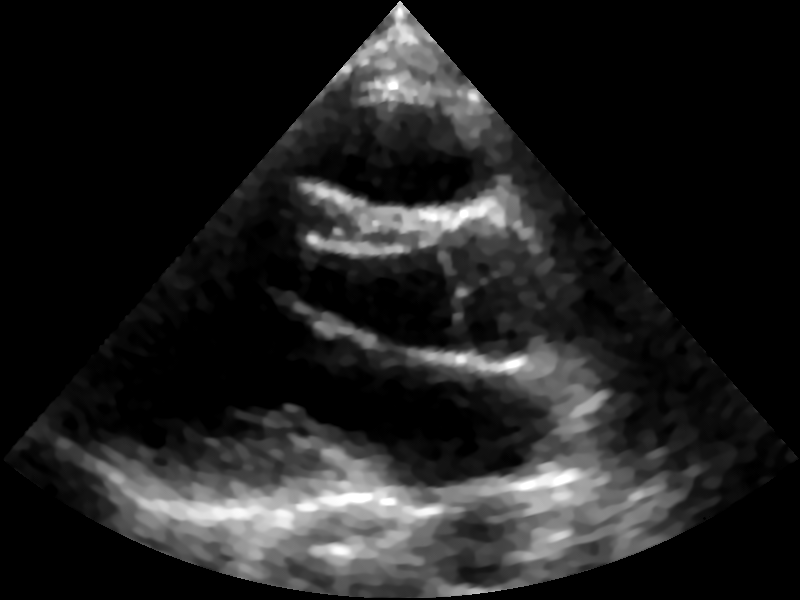
\includegraphics[width=\textwidth]{figures/cardiac1_osrad.png}};
      \spy on (0.05, 0.05) in node [redwindow, anchor=north] at ($(figA.south)$);
    \end{tikzpicture}
    \caption{OSRAD}
  \end{subfigure}%
  \begin{subfigure}[b]{0.15\textwidth}
    \begin{tikzpicture}[
        spy using outlines={%
          rectangle, magnification=3,size=\textwidth,
          every spy on node/.append style={transparentwindow}
        }
      ]
      \node (figA) at (0.0,0.0) {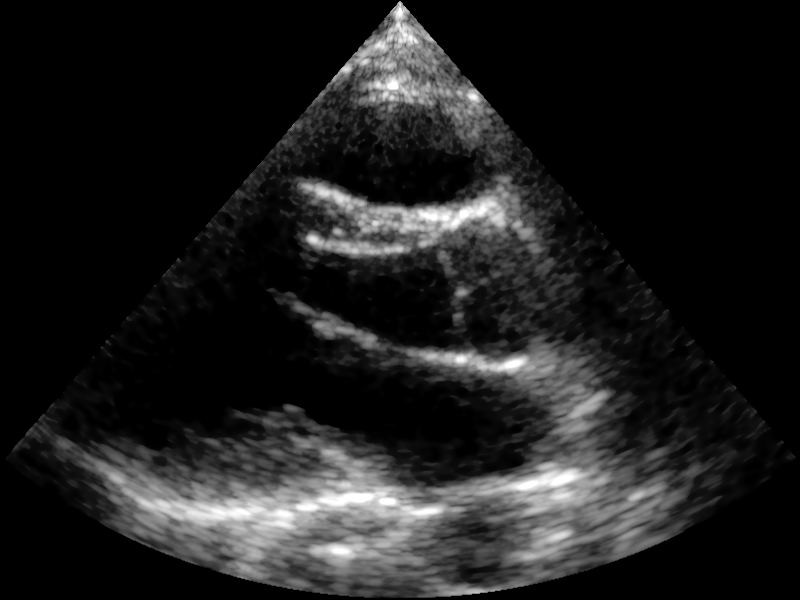
\includegraphics[width=\textwidth]{figures/cardiac1_admss.png}};
      \spy on (0.05, 0.05) in node [redwindow, anchor=north] at ($(figA.south)$);
    \end{tikzpicture}
    \caption{ADMSS}
  \end{subfigure}%
  \begin{subfigure}[b]{0.15\textwidth}
    \begin{tikzpicture}[
        spy using outlines={%
          rectangle, magnification=3,size=\textwidth,
          every spy on node/.append style={transparentwindow}
        }
      ]
      \node (figA) at (0.0,0.0) {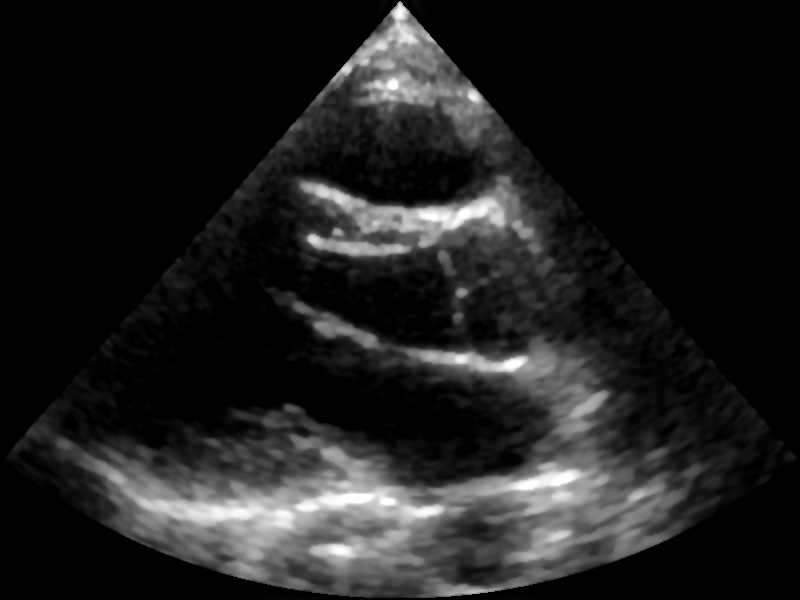
\includegraphics[width=\textwidth]{figures/cardiac1_lpndsf.png}};
      \spy on (0.05, 0.05) in node [redwindow, anchor=north] at ($(figA.south)$);
    \end{tikzpicture}
    \caption{LPNDSF}
  \end{subfigure}%
  \begin{subfigure}[b]{0.15\textwidth}
    \begin{tikzpicture}[
        spy using outlines={%
          rectangle,magnification=3,size=\textwidth,
          every spy on node/.append style={transparentwindow}
        }
      ]
      \node (figA) at (0.0,0.0) {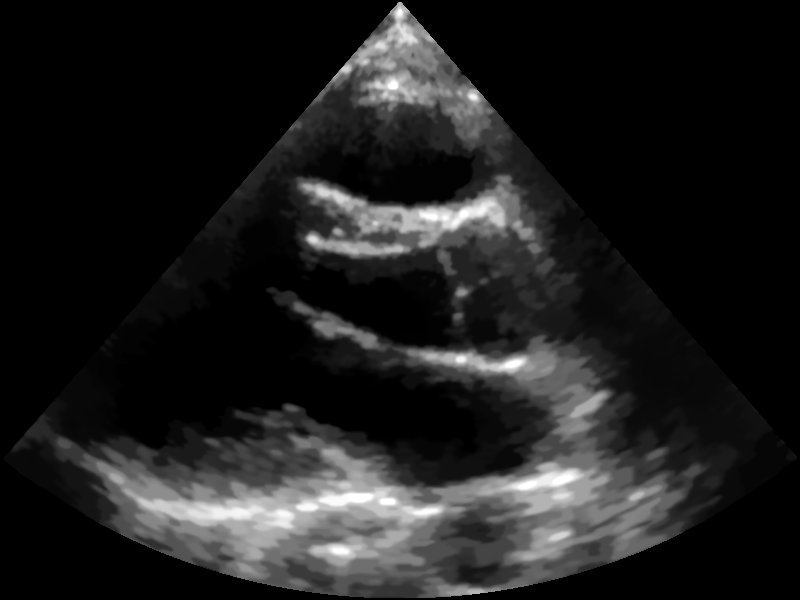
\includegraphics[width=\textwidth]{figures/cardiac1_mnlm.png}};
      \spy on (0.05, 0.05) in node [redwindow, anchor=north] at ($(figA.south)$);
    \end{tikzpicture}
    \caption{MNLM}
  \end{subfigure}%
  \begin{subfigure}[b]{0.15\textwidth}
    \begin{tikzpicture}[
        spy using outlines={%
          rectangle,magnification=3,size=\textwidth,
          every spy on node/.append style={transparentwindow}
        }
      ]
      \node (figA) at (0.0,0.0) {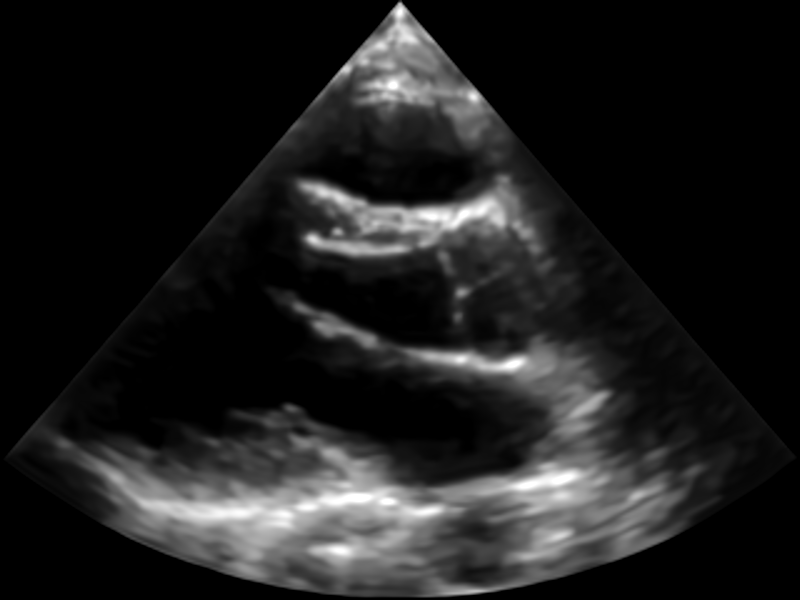
\includegraphics[width=\textwidth]{figures/cardiac1_nllr.png}};
      \spy on (0.05, 0.05) in node [redwindow, anchor=north] at ($(figA.south)$);
    \end{tikzpicture}
    \caption{NLLR}
  \end{subfigure}%
  \begin{subfigure}[b]{0.15\textwidth}
    \begin{tikzpicture}[
        spy using outlines={%
          rectangle,magnification=3,size=\textwidth,
          every spy on node/.append style={transparentwindow}
        }
      ]
      \node (figA) at (0.0,0.0) {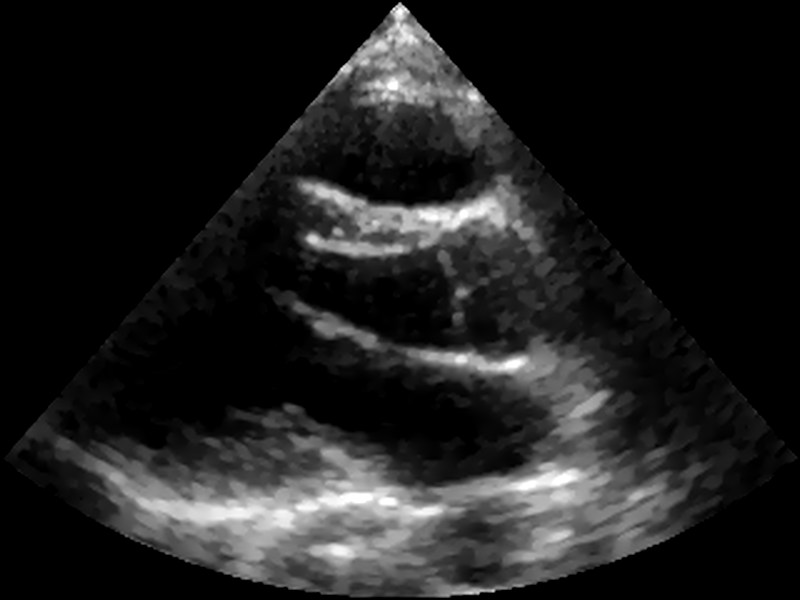
\includegraphics[width=\textwidth]{figures/cardiac1_pfdtv.png}};
      \spy on (0.05, 0.05) in node [redwindow, anchor=north] at ($(figA.south)$);
    \end{tikzpicture}
    \caption{PFDTV}
  \end{subfigure}\\
  %% \begin{subfigure}[b]{0.15\textwidth}
  %%   \begin{tikzpicture}[
  %%       spy using outlines={%
  %%         rectangle,magnification=3,size=\textwidth,
  %%         every spy on node/.append style={transparentwindow}
  %%       }
  %%     ]
  %%     \node (figA) at (0.0,0.0) {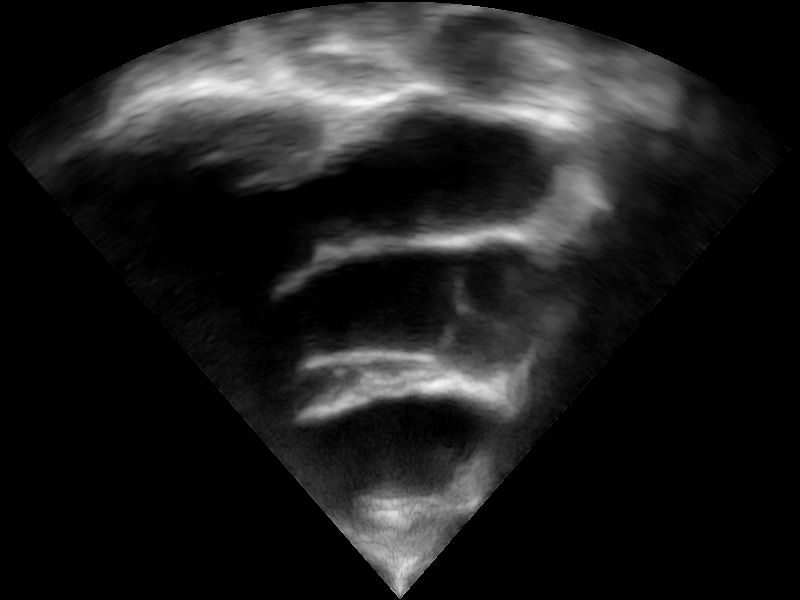
\includegraphics[width=\textwidth, trim={4cm 4cm 4cm 0cm}, clip]{figures/cardiac1_clpdQ.png}};
  %%     \spy on (0.05, 0.05) in node [redwindow, anchor=north] at ($(figA.south)$);
  %%   \end{tikzpicture}
  %%   \caption{CLPD-SSNR}
  %% \end{subfigure}%
  \begin{subfigure}[b]{0.15\textwidth}
    \begin{tikzpicture}[
        spy using outlines={%
          rectangle,magnification=3,size=\textwidth,
          every spy on node/.append style={transparentwindow}
        }
      ]
      \node (figA) at (0.0,0.0) {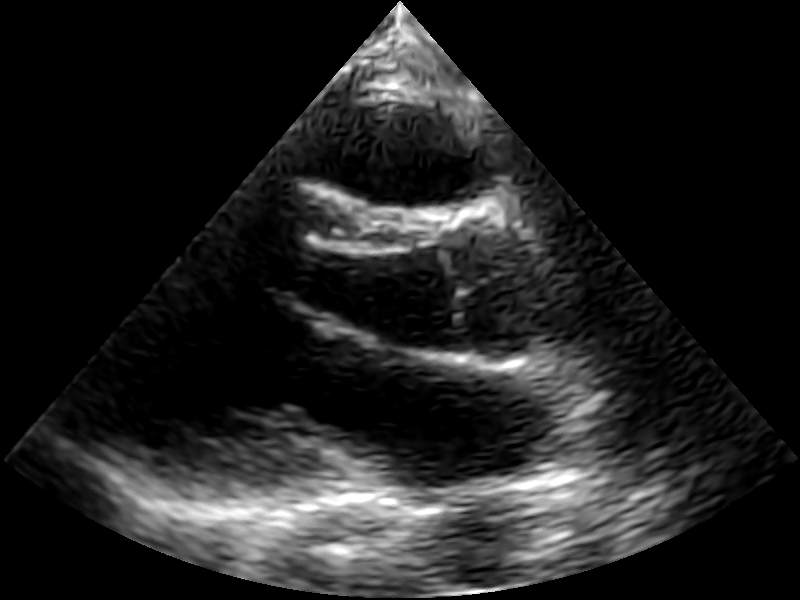
\includegraphics[width=\textwidth]{figures/cardiac1_clpda.png}};
      \spy on (0.05, 0.05) in node [redwindow, anchor=north] at ($(figA.south)$);
    \end{tikzpicture}
    \caption{CLPD-A}
  \end{subfigure}%
  \begin{subfigure}[b]{0.15\textwidth}
    \begin{tikzpicture}[
        spy using outlines={%
          rectangle,magnification=3,size=\textwidth,
          every spy on node/.append style={transparentwindow}
        }
      ]
      \node (figA) at (0.0,0.0) {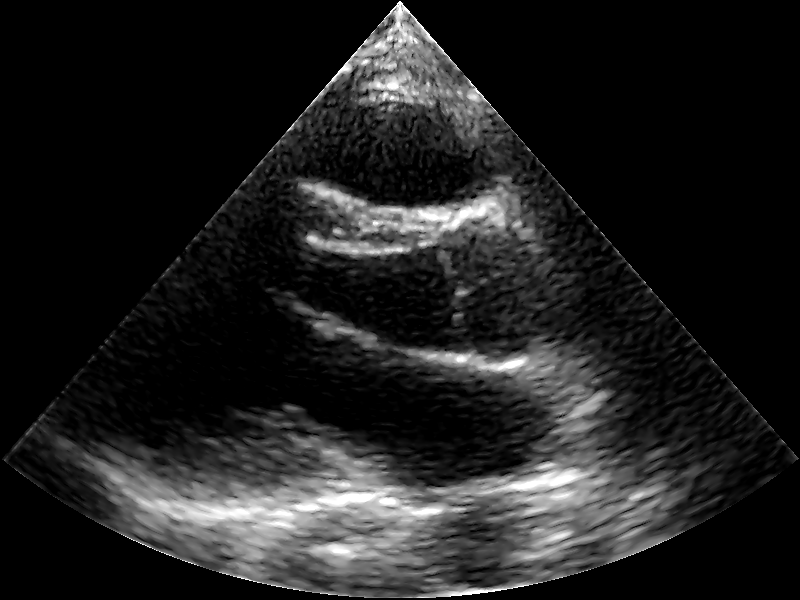
\includegraphics[width=\textwidth]{figures/cardiac1_clpdb.png}};
      \spy on (0.05, 0.05) in node [redwindow, anchor=north] at ($(figA.south)$);
    \end{tikzpicture}
    \caption{CLPD-B}
  \end{subfigure}%
  \begin{subfigure}[b]{0.15\textwidth}
    \begin{tikzpicture}[
        spy using outlines={%
          rectangle,magnification=3,size=\textwidth,
          every spy on node/.append style={transparentwindow}
        }
      ]
      \node (figA) at (0.0,0.0) {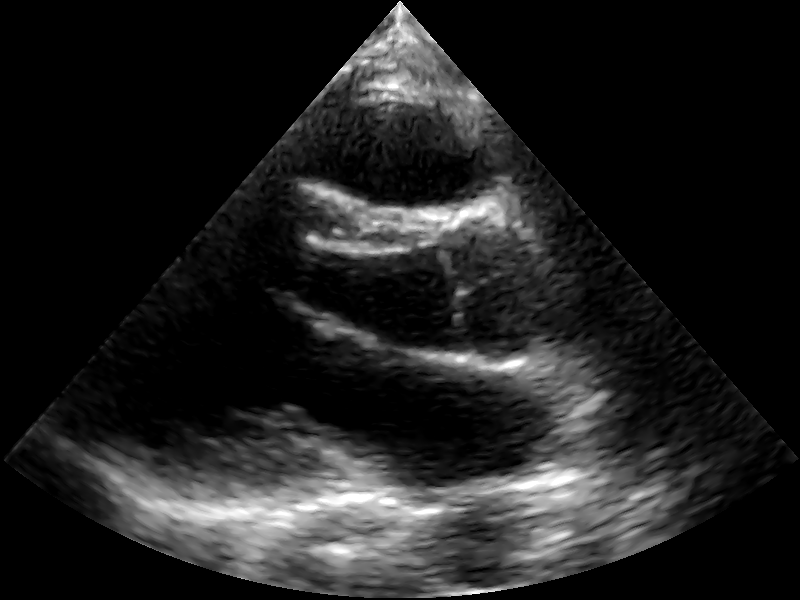
\includegraphics[width=\textwidth]{figures/cardiac1_clpdc.png}};
      \spy on (0.05, 0.05) in node [redwindow, anchor=north] at ($(figA.south)$);
    \end{tikzpicture}
    \caption{CLPD-C}
  \end{subfigure}%
  \begin{subfigure}[b]{0.15\textwidth}
    \begin{tikzpicture}[
        spy using outlines={%
          rectangle,magnification=3,size=\textwidth,
          every spy on node/.append style={transparentwindow}
        }
      ]
      \node (figA) at (0.0,0.0) {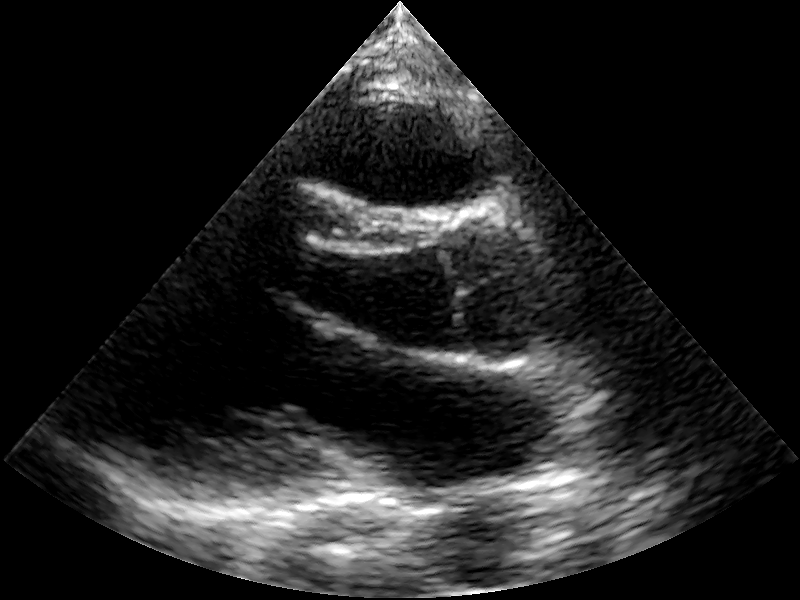
\includegraphics[width=\textwidth]{figures/cardiac1_clpdd.png}};
      \spy on (0.05, 0.05) in node [redwindow, anchor=north] at ($(figA.south)$);
    \end{tikzpicture}
    \caption{CLPD-D}
  \end{subfigure}%
  \begin{subfigure}[b]{0.15\textwidth}
    \begin{tikzpicture}[
        spy using outlines={%
          rectangle,magnification=3,size=\textwidth,
          every spy on node/.append style={redwindow}
        }
      ]
      \node (figA) at (0.0,0.0) {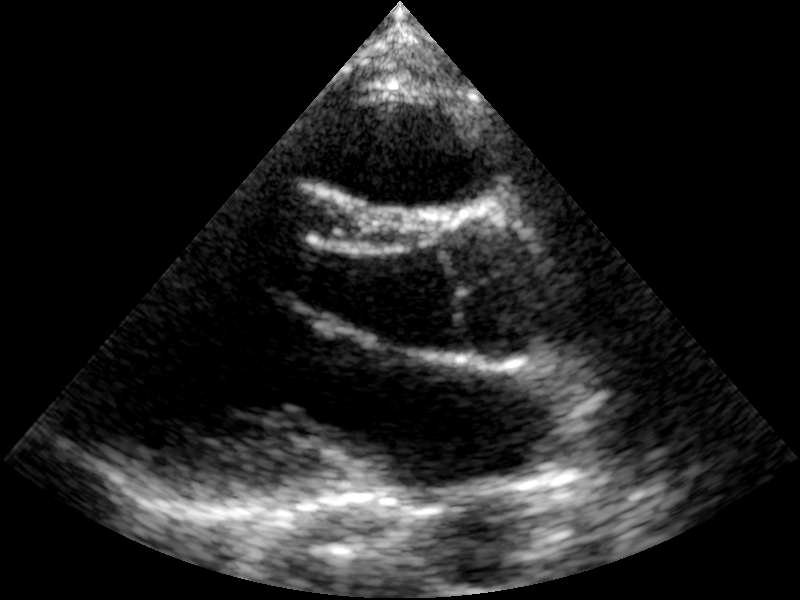
\includegraphics[width=\textwidth]{figures/cardiac1.png}};
      \spy on (0.05, 0.05) in node [redwindow, anchor=north] at ($(figA.south)$);
    \end{tikzpicture}
    \caption{Original}
  \end{subfigure}
  \caption{Results on echocardiography parasternal long-axis view.}\label{fig:cardiac1}
  \vspace{-0.1in}
\end{figure*}

%%% Local Variables:
%%% TeX-master: "master"
%%% End:

%
\subsubsection{Quantitative Results}
The quantatitive results using objective performance metrics are shown in~\cref{table:liver1}.
First, we can see that the SSNR values obtained using the CLPDs are worse compared to the baselines except for CLPD-obj., which is natural since it was explicitly tuned to obtain a high SSNR.
This shows that, while it is definitely possible to obtain a high SSNR with the CLPD, none of the sonographers preferred a high SSNR.
Instead, they preferred to preserve some level of speckle noise.
In contrast, all of the baselines except for ADMSS obtained higher SSNR.
In particular, the MNLM obtains the highest leverl of SSNR, which supports the statement that non-local means methods are excellent at removing speckle (which is unfortunately, not desirable).

Meanwhile, when looking at other metrics than the SSNR, the results look quite different.
The CLPDs obtained both high SSIM and high \(S_3\) overall.
Only ADMSS obtained a high SSIM, which is natural since it refrains diffusing tissues.
CLPDs on the other hand all resulted in high levels of SSIMs, which shows that sonographers strongly prefer images that do not look different from the original image.

Lastly, when looking at the \(S_3\) metric, we can see that all CLPDs obtained much higher values.
This shows that the CLPD is capable of conserving sharpness, and that sonographers strongly prefer sharp-looking images.
In fact, many of the participating sonographers explicitly stated that they ``do not want to trade sharpness for less speckle''.
Our results clearly reflect this sentiment.
For this reason, while the NLLR is very good at reinforcing strucutres and reducing speckle, it results in images that are significantly blurry both qualititatively and quantitatively (according to \(S_3\)), which limits its clinical value.

\begin{table}
  \centering
  \caption{Quantatitive Results on Echocardiographic 4-Chamber View}\label{table:cardiac3}
  \setlength{\tabcolsep}{3pt}
  \begin{threeparttable}
  \begin{tabular}{llrrrrr}
    \toprule
    & \multicolumn{1}{c}{\textbf{Algorithm}}
    & \multicolumn{1}{c}{\textbf{gCNR}}
    & \multicolumn{1}{c}{\textbf{CNR}}
    & \multicolumn{1}{c}{\textbf{SNR}}
    & \multicolumn{1}{c}{\textbf{SSIM}}
    & \multicolumn{1}{c}{\(\mathbf{S_{3}}\)}\\
    & \multicolumn{1}{c}{}
    & \multicolumn{1}{c}{}
    & \texttt{[dB]}
    & \texttt{[dB]}
    & \multicolumn{1}{c}{}
    & \multicolumn{1}{c}{} \\\midrule
    \multirow{6}{*}{Baselines}
    & OSRAD  & 0.490          & -1.62          & 4.51          & 0.891          & 0.500 \\
    & ADMSS  & 0.467          & -1.67          & 4.33          & \textbf{0.967} & 0.204 \\
    & LPNDSF & 0.473          & -1.67          & 4.39          & 0.868          & 0.458 \\
    & MNLM   & \textbf{0.534} & \textbf{-1.61} & 4.42          & 0.918          & 0.414 \\
    & NLLR   & \textbf{0.501} & \textbf{-1.60} & 4.61          & 0.857          & 0.042\\
    & PFDTV  & 0.480          & -1.65          & 4.49          & 0.865          & 0.155 \\\midrule
    \multirow{4}{*}{This work}
    & CLPD-A & 0.484          & -1.64          & \textbf{4.64} & \textbf{0.957} & \textbf{0.858} \\
    & CLPD-B & \textbf{0.496} & \textbf{-1.55} & \textbf{4.69} & \textbf{0.949} & \textbf{0.685} \\
    & CLPD-E & 0.476          & -1.63          & \textbf{4.61} & \textbf{0.961} & \textbf{0.507} \\
    & CLPD-F & \textbf{0.507} & \textbf{-1.50} & \textbf{4.79} & 0.920          & \textbf{0.705} \\\bottomrule
  \end{tabular}
  \begin{tablenotes}
    \item[*] The performance of the top 4 algorithms for each metric are shown in bold face.
  \end{tablenotes}
  \end{threeparttable}
  \vspace{-0.2in}
\end{table}
%
\subsection{Results on Echocardiographic 4-Chamber View}
%We now present results on a sequence of echocardiographic 4-chamber view images.

\subsubsection{Qualititative Results}
A single frame from each processed result is shown in~\cref{fig:cardiac3}.
Similarly with the liver image, CLPD-A to CLPD-F turned out to be the least blurry.
Unlike the liver image, however, some of the expert tuned CLPDs showed strong speckle reduction.
For example, CLPD-F shows the cleanest myocardium wall among all methods.
Despite the strong smoothing effect, it does not result in blurry images such as NLLR, which shows the effectiveness of the cascaded Laplacian pyramid approach.

In addition, CLPDs resulted in smooth myocardium edges, thanks to the multiscale analysis of the Laplacian pyramid.
In contrast, other methods result in jiggly myocardium edges due to structural dagmaes caused by speckle.
While NLLR results in the best structural enhancement, the resulting blurriness shadows its benefits.

Meanwhile, CLPD-A results in amplified fine details.
Indeed, the cardiologist (A) who tuned CLPD-A expressed his preference for fine details such as papillary muscles.
This shows the preferential difference between cardiologist and sonographers.
Overall, the results on the echocardiographic 4-chamber view show that image enhancement methods need to be tuned, not only to each individual, but also each clinical task.

\subsubsection{Quantitative Results}
%We now discuss the quantitative results on the echocardiographic 4-chamber image.

For the echocardiographic images, correctly recognizing different anatomical structures and thier borders is clinically important.
Therefore, unlike the liver image, speckle reduction and contrast enhancement is more relevant.
This is clearly reflected in~\cref{table:cardiac3}.
All CLPD settings showed the highest SNR on the myocardium wall.
In terms of contrast, sonographer B and F showed preference towards high gCNR and CNR.
However, CLPDs still achieved high SSIM and \(S_3\).

Among the considered baselines, MNLM and NLLR achieved the highers contrast.
Still, both methods are known to be good at removing speckle.
However, they both resulted in low sharpness, where NLLR resulted in an unbelievely low \(S_3\) value.
Meanwhile, except for NLLR, all methods did not achieve a high SNR.
Although this is expected with ADMSS since it deliberately avoids reducing speckle on structural regions, the low SNR of MNLM is counter-intuitive.
From visual inspection, this seems to be a result of MNLM and other methods not improving the homogeneity of similar anatomical regions.
NLLR and CLPDs, on ther other hand, improve the structural homogeneity.
This shows the importance of structural enhancement for echocardiographic images, which CLPDs achieve by coherence enhancement in higher scales.

\subsection{Results on Echocardocraphic Parasternal Long-Axis View}
Finally, we present qualitative results on an echocardocraphic parasternal long-axis view sequence.
The parasternal long-axis view has many clinically relevant fine details such as the mitral valve and the aortic valve.
These fine details, however, are difficult to differentiate from speckle and clutter.

The results are shown in~\cref{fig:cardiac3}.
Unlike the echocardiographic 4-chamber view, all CLPDs amplify fine-details regardless of speckle and clutter.
Flow-like artifacts resulting from aggressive coherence enhancement are clearly visible near the aortic valve.
As a result, the edges of the interventricular septum are enhanced.

%%% Local Variables:
%%% TeX-master: "master"
%%% End:


\section{Related Works}\label{section:relatedworks}
\subsubsection{Medical Ultrasound Image Enhancements}
\cite{hemmsen_ultrasound_2010} propose a software for comparing medical images using the double-stimulus continuous-quality scale.
%Evaluating automatic time-gain adjustment algorithms~\cite{axelsen_evaluation_2010, moshavegh_advanced_2015}.

An important issue is that speckle reduction filter tend to generate blurry results.
\cite{deng_speckle_2011, wong_monte_2012, hu_cluster_2016, singh_hybrid_2017, nagare_multi_2017} tend to generate blurry images regardless of the speckle reduction performance.
Especially, despite the superior performance of the hybrid filter~\cite{singh_hybrid_2017}.

\subsubsection{Design Galleries and Preferential Bayesian Optimization}

\subsubsection{Design Galleries and Preferential Bayesian Optimization}

%%% Local Variables:
%%% TeX-master: "master"
%%% End:



\section{Disscusions}\label{section:conclusion}
Understanding and optimizing the subjective quality metrics of sonographers is a crucial task for improving the clinical performance of medical ultrasound imaging systems.
In this work, we have presented the \textsc{Ultrasound Design Gallery}, a graphical tool for inferring and optimizing the subjective metrics of sonographers.
By leveraging machine learning and Bayesian optimization, our tool enables automatic, personalized, task-specific tuning of ultrasound imaging systems.
We have demonstrated the utility of our tool by letting sonographers tune the parameters of the \textsc{cascaded laplacian pyramid diffusion} (CLPD), which is a novel medical ultrasound image enhancement algorithm.
The CLPD enables sharing of information between different image scales and seamless integration of conventional image enhancement filters.

Our experimental results have shown that individual sonographers exhibit different visual preferences.
In addition, their preference changes greatly depending on the clinical task and scanning view.
Therefore, personalized and task-specific tuning of ultrasound image enhancement algorithms, possibly using the USDG, is crucial for optimal clinical performance.

While image sharpness/blurriness has not been a focus in medical ultrasound images, we have shown that sonographers prioritize natural and sharp-looking images.
Unfortunately, most conventional blurriness metrics are calibrated to natural images.
Therefore, we point out that quantifying the blurriness of medical ultrasound images is an interesting open problem.
In addition, for understanding and optimizing the preference of sonographers and radiologists, methods developed in psychology such as~\cite{NIPS2007_89d4402d} could be interesting to explore.

%%% Local Variables:
%%% TeX-master: "master"
%%% End:


% use section* for acknowledgment
\ifCLASSOPTIONcompsoc
  % The Computer Society usually uses the plural form
  \section*{Acknowledgments}
\else
  % regular IEEE prefers the singular form
  \section*{Acknowledgment}
\fi

This work was only made possible by the support and voluntary contribution of the sonographers at Kangbuk Samsung Hospital.
The authors are also grateful to Jeonggyu Kang and Yangmo Yoo for their feedback on our image enhancement algorithm, Heechul Yoon for detailed comments on our paper, Petrus Mikkola for discussions about projective preferential Bayesian optimization, and Aki Vehtari for discussions about Gaussian processes.

This work was supported by the Korea Medical Device Development Fund grant funded by the Korea government (the Ministry of Science and ICT, the Ministry of Trade, Industry and Energy, the Ministry of Health \& Welfare, the Ministry of Food and Drug Safety) (Project Number: 1711137879, KMDF\_PR\_20200901\_0009)

% Can use something like this to put references on a page
% by themselves when using endfloat and the captionsoff option.
\ifCLASSOPTIONcaptionsoff
  \newpage
\fi


% trigger a \newpage just before the given reference
% number - used to balance the columns on the last page
% adjust value as needed - may need to be readjusted if
% the document is modified later
%\IEEEtriggeratref{8}
% The "triggered" command can be changed if desired:
%\IEEEtriggercmd{\enlargethispage{-5in}}

% references section

% can use a bibliography generated by BibTeX as a .bbl file
% BibTeX documentation can be easily obtained at:
% http://mirror.ctan.org/biblio/bibtex/contrib/doc/
% The IEEEtran BibTeX style support page is at:
% http://www.michaelshell.org/tex/ieeetran/bibtex/
%\bibliographystyle{IEEEtran}
% argument is your BibTeX string definitions and bibliography database(s)
%\bibliography{IEEEabrv,../bib/paper}
%
% <OR> manually copy in the resultant .bbl file
% set second argument of \begin to the number of references
% (used to reserve space for the reference number labels box)
%\vspace{-0.15in}
\bibliographystyle{IEEEtran}
\bibliography{bstcontrol,references}

% biography section
% 
% If you have an EPS/PDF photo (graphicx package needed) extra braces are
% needed around the contents of the optional argument to biography to prevent
% the LaTeX parser from getting confused when it sees the complicated
% \includegraphics command within an optional argument. (You could create
% your own custom macro containing the \includegraphics command to make things
% simpler here.)
%\begin{IEEEbiography}[{\includegraphics[width=1in,height=1.25in,clip,keepaspectratio]{mshell}}]{Michael Shell}
% or if you just want to reserve a space for a photo:


\begin{IEEEbiography}[{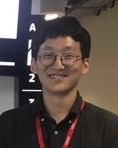
\includegraphics[width=1in,height=1.25in,clip,keepaspectratio]{figures/author_krk}}]{Kyurae~Kim} (Member, IEEE) received the B.S. degree in electronics engineering from Sogang University, Seoul, South Korea, in 2021.

  He worked as an undergraduate researcher at Samsung Seoul Hospital, Seoul, South Korea from 2017 to 2020.
  He currently works as a Research Associate at the Department of Electrical Engineering and Electronics, University of Liverpool, Liverpool, United Kingdom.
  His research interests include Bayesian inference methods, probabilistic machine learning, parallel computing, and image processing.

  Kim is a member of the Association for Computing Machinery (ACM).
\end{IEEEbiography}
\vspace{-0.3in}

\begin{IEEEbiography}[{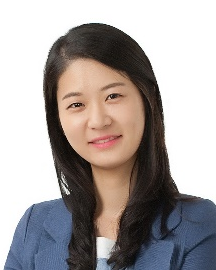
\includegraphics[width=1in,height=1.25in,clip,keepaspectratio]{figures/author_mrl}}]{Miran Lee} received the B.S. degree in Health Science from Korea University, Seoul, South Korea, in 2008, and the M.S. degree from the Department of Biomedical Sciences, Korea University, Seoul, South Korea, in 2014.

  She has been working as a Cardiac Sonographer at the Department of Total Healthcare Center, Kangbuk Samsung Hospital, Sungkyunkwan University School of Medicine, since 2013.
  She is currently a Ph.D. student in Electronics Engineering at Sogang University. 
  Her main research interests are in developing efficient artificial intelligence architectures for ultrasound systems and deep learning in medical images.
\end{IEEEbiography}
\vspace{-0.3in}

\begin{IEEEbiography}[{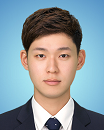
\includegraphics[width=1in,height=1.25in,clip,keepaspectratio]{figures/author_kkl}}]{Kunkyu Lee}
received the B.S. and M.S degrees from the Department of Electronic Engineering, Sogang University, Seoul, South Korea, in 2016 and 2018, respectively.

He is currently a Ph.D. student in Electronics Engineering at Sogang University.
His main research interests are the development of efficient portable ultrasound imaging system, the efficient architecture of artificial intelligence with ultrasound system and Deep learning image processing in medical images.
\end{IEEEbiography}
\vspace{-0.3in}

\begin{IEEEbiography}[{\includegraphics[width=1in,height=1.25in,clip,keepaspectratio]{figures/author_mk}}]{Min Kim} received the Ph.D. degree in the Department of Electronic Engineering, the Sogang University, Seoul, South Korea. 

From 2017 to 2019, he worked as a research professor of the Department of Electronic Engineering, Sogang University. 
He is currently the Director of the Research Institute of Hansono, Seoul, South Korea. 
His research interests include ultrasound image processing and hand-held ultrasound systems for point-of-care ultrasound.
\end{IEEEbiography}
\vspace{-0.3in}

\begin{IEEEbiography}[{\includegraphics[width=1in,height=1.25in,clip,keepaspectratio]{figures/author_tks}}]{Tai-kyong Song} (Member, IEEE) received the B.S. degree in electronic engineering from Sogang University, Seoul, South Korea, in 1984, and the M.S. and Ph.D. degrees from the Department of Electrical and Electronic Engineering, Korea Advanced Institute of Science and Technology (KAIST), Seoul, in 1985 and 1990, respectively. 

  He worked as a Research Fellow at the Department of Physiology and Biophysics, Mayo Clinic, Rochester, MN, USA, for two years before appointed as an Adjunct Professor with the Department of Information and Communication Engineering, KAIST, from 1993 to 1995.
  He worked as a Staff Scientist at Siemens Healthcare, Medical-System Inc., Issaquah, WA, USA, from 1995 to 1997.
  He joined the Department of Electronic Engineering, Sogang University as an Assistant Professor, in 1997.
  He was promoted to a professor, in 2006. He has been the Director of the Medical Solution Institute, Sogang University, since 2000.
  His research interests include medical ultrasound imaging and therapy, portable ultrasound imaging systems, ultrafast 3-D scanning algorithms, photoacoustic imaging and its translational research, digital signal and image processing, and multimodal imaging system for preventive and surgical applications.
  He is currently the President of the Korean Medical Ultrasound Link, South Korea.
  He has served as an Associate Editor for the \textsc{IEEE Transactions on Ultrasonics, Ferroelectrics, and Frequency Control}, from 2002 to 2007.

  Prof. Song is a member of the National Academy of Engineering of Korea (NAEK), South Korea. 
\end{IEEEbiography}

%%% Local Variables:
%%% TeX-master: "master"
%%% End:


% if you will not have a photo at all:
%\begin{IEEEbiographynophoto}{Min Kim}
%\end{IEEEbiographynophoto}

% insert where needed to balance the two columns on the last page with
% biographies
%\newpage

\end{document}


